% !TEX program = pdflatex
\documentclass[12pt, a4paper, onecolumn, oneside]{report}

%%=============================================================
%% PACKAGES
%%=============================================================
\usepackage[indonesian]{babel}
\usepackage[utf8]{inputenc}
\usepackage[T1]{fontenc}
\usepackage{setspace}
\usepackage[raggedrightboxes]{ragged2e}
\usepackage{graphicx}
\graphicspath{{../Project/gambar/}{gambar/}{../Rancangan/Mermaid/}{../Rancangan/Wireframe/}}
\usepackage{float}
\usepackage{indentfirst}
\setlength\parindent{1cm}
\usepackage{pslatex}
\usepackage{tabularx}
\usepackage{multirow}
\usepackage{colortbl}
\usepackage{xcolor}
\usepackage{amsmath}
\usepackage{amssymb}
\usepackage{enumitem}
\usepackage{longtable}
\usepackage{xltabular}
\usepackage{booktabs}
\usepackage{listings}
\lstset{
  language=Python,
  basicstyle=\ttfamily\footnotesize,
  keywordstyle=\bfseries,
  commentstyle=\itshape\color{gray},
  showstringspaces=false,
  breaklines=true,
  breakatwhitespace=true,
  frame=single,
  numbers=left,
  numberstyle=\tiny,
  xleftmargin=2em,
  framexleftmargin=1.5em,
  captionpos=b,
  tabsize=2,
  aboveskip=0.8em,
  belowskip=0.8em
}
\renewcommand{\lstlistingname}{Kode Program}
\usepackage[font=small, format=plain, labelfont=bf, up, textfont=up]{caption}
\usepackage{subcaption}
\usepackage{geometry}
\usepackage{fancyhdr}
\usepackage{titlesec}
\usepackage{tocloft}
\usepackage{ifthen}
\usepackage[hidelinks]{hyperref}
\usepackage{tikz}
\usepackage{pdflscape}
\usetikzlibrary{shapes.geometric, arrows.meta, positioning, shapes.multipart}

%%=============================================================
%% LAYOUT
%%=============================================================
\geometry{a4paper, left=4cm, top=4cm, right=3cm, bottom=3cm}

\setlength{\headheight}{14.5pt}
\fancyhf{}
\rhead{\thepage}
\renewcommand{\headrulewidth}{0pt}
\renewcommand{\footrulewidth}{0pt}

\tolerance=1
\emergencystretch=\maxdimen
\hyphenpenalty=10000
\hbadness=10000

%%=============================================================
%% TOC FORMAT
%%=============================================================
\cftsetpnumwidth{1.5em}
\cftsetrmarg{2em}
\setlength{\cftsecnumwidth}{2.5em}
\setlength{\cftsubsecnumwidth}{4em}
\setlength{\cftsubsubsecindent}{4.5em}
\setlength{\cftsubsubsecnumwidth}{4.8em}
\renewcommand{\cftchapdotsep}{\cftdotsep}
\setlength{\cftbeforechapskip}{3pt}
\renewcommand\cftchappresnum{BAB }
\renewcommand\cftchapaftersnum{}
\newlength\mylen
\settowidth\mylen{\bfseries BAB III :\ }
\cftsetindents{chap}{0pt}{\mylen}

%%=============================================================
%% CHAPTER & SECTION FORMAT
%%=============================================================
\titleformat{\chapter}{\doublespacing\fontsize{14pt}{16pt}\bfseries}%
    {\MakeUppercase{\chaptertitlename\ \Roman{chapter}}\filcenter}{0.15cm}{\centering\uppercase}
\titleformat{\section}{\fontsize{12}{14}\bfseries}{\thesection}{0.4cm}{}
\titleformat{\subsection}{\fontsize{12}{14}\bfseries}{\thesubsection}{0.675cm}{}
\titleformat{\subsubsection}{\fontsize{12}{14}\bfseries}{\thesubsubsection}{0.675cm}{}
\titlespacing*{\chapter}{0pt}{-1cm}{20pt}
\titlespacing*{\section}{0pt}{1cm}{0pt}
\titlespacing*{\subsection}{0pt}{0.75cm}{0pt}
\titlespacing*{\subsubsection}{0pt}{0.75cm}{0pt}

\setcounter{secnumdepth}{3}
\setcounter{tocdepth}{3}

\captionsetup[figure]{labelsep=space}
\captionsetup[table]{labelsep=space}
\renewcommand{\thefigure}{\arabic{chapter}.\arabic{figure}}
\renewcommand{\thetable}{\arabic{chapter}.\arabic{table}}

%%=============================================================
%% LIST FORMAT
%%=============================================================
\setlist{nosep}
\newenvironment{packed_enum}{
    \begin{enumerate}[leftmargin=1.5\parindent]
        \setlength{\itemsep}{0pt}
        \setlength{\parskip}{0pt}
        \setlength{\parsep}{0pt}
        }{\end{enumerate}}

\newenvironment{packed_item}{
    \begin{itemize}[leftmargin=1.375\parindent]
        \setlength{\itemsep}{0pt}
        \setlength{\parskip}{0pt}
        \setlength{\parsep}{0pt}
        }{\end{itemize}}
%%=============================================================
%% EQUATION NUMBERING
%%=============================================================
\makeatletter
\renewcommand{\theequation}{\arabic{chapter}.\arabic{equation}}
\renewcommand{\@eqnnum}{\theequation}
\def\tagform@#1{\maketag@@@{(#1)}}
\makeatother

%% Nomor bab Romawi (konsisten Daftar Isi vs judul bab),
%% subbab/gambar/tabel/persamaan tetap Arab.
\renewcommand{\thechapter}{\Roman{chapter}}
\renewcommand{\thesection}{\arabic{chapter}.\arabic{section}}

%%=============================================================
%% DOCUMENT
%%=============================================================
\begin{document}

%%-------------------------------------------------------------
%% HALAMAN JUDUL
%%-------------------------------------------------------------
\begin{titlepage}
\thispagestyle{empty}
\begin{spacing}{1.0}
\begin{center}

{\fontsize{14}{16}\selectfont\bfseries SKRIPSI}

\vspace{1.5cm}

{\fontsize{14}{16}\selectfont\bfseries
RANCANG BANGUN APLIKASI \textit{POINT OF SALE}\\[4pt]
DENGAN FITUR PREDIKSI PENJUALAN HARIAN\\[4pt]
MENGGUNAKAN METODE \textit{LONG SHORT-TERM MEMORY} (LSTM)}

\vspace{2.5cm}


\includegraphics[width=3.5cm]{logo-pnl-skripsi}

\vspace{2.5cm}

Disusun oleh:\\[0.5cm]
{\bfseries MUHAMMAD KHOLIS\\[4pt]
2022573010098}

\vfill

{\bfseries
PROGRAM STUDI TEKNIK INFORMATIKA\\[4pt]
JURUSAN TEKNOLOGI INFORMASI DAN KOMPUTER\\[4pt]
POLITEKNIK NEGERI LHOKSEUMAWE\\[4pt]
TAHUN 2026}

\end{center}
\end{spacing}
\end{titlepage}

%%-------------------------------------------------------------
%% HALAMAN PENGESAHAN
%%-------------------------------------------------------------
\newgeometry{left=0cm,right=0cm,top=0cm,bottom=0cm}
\thispagestyle{empty}
\noindent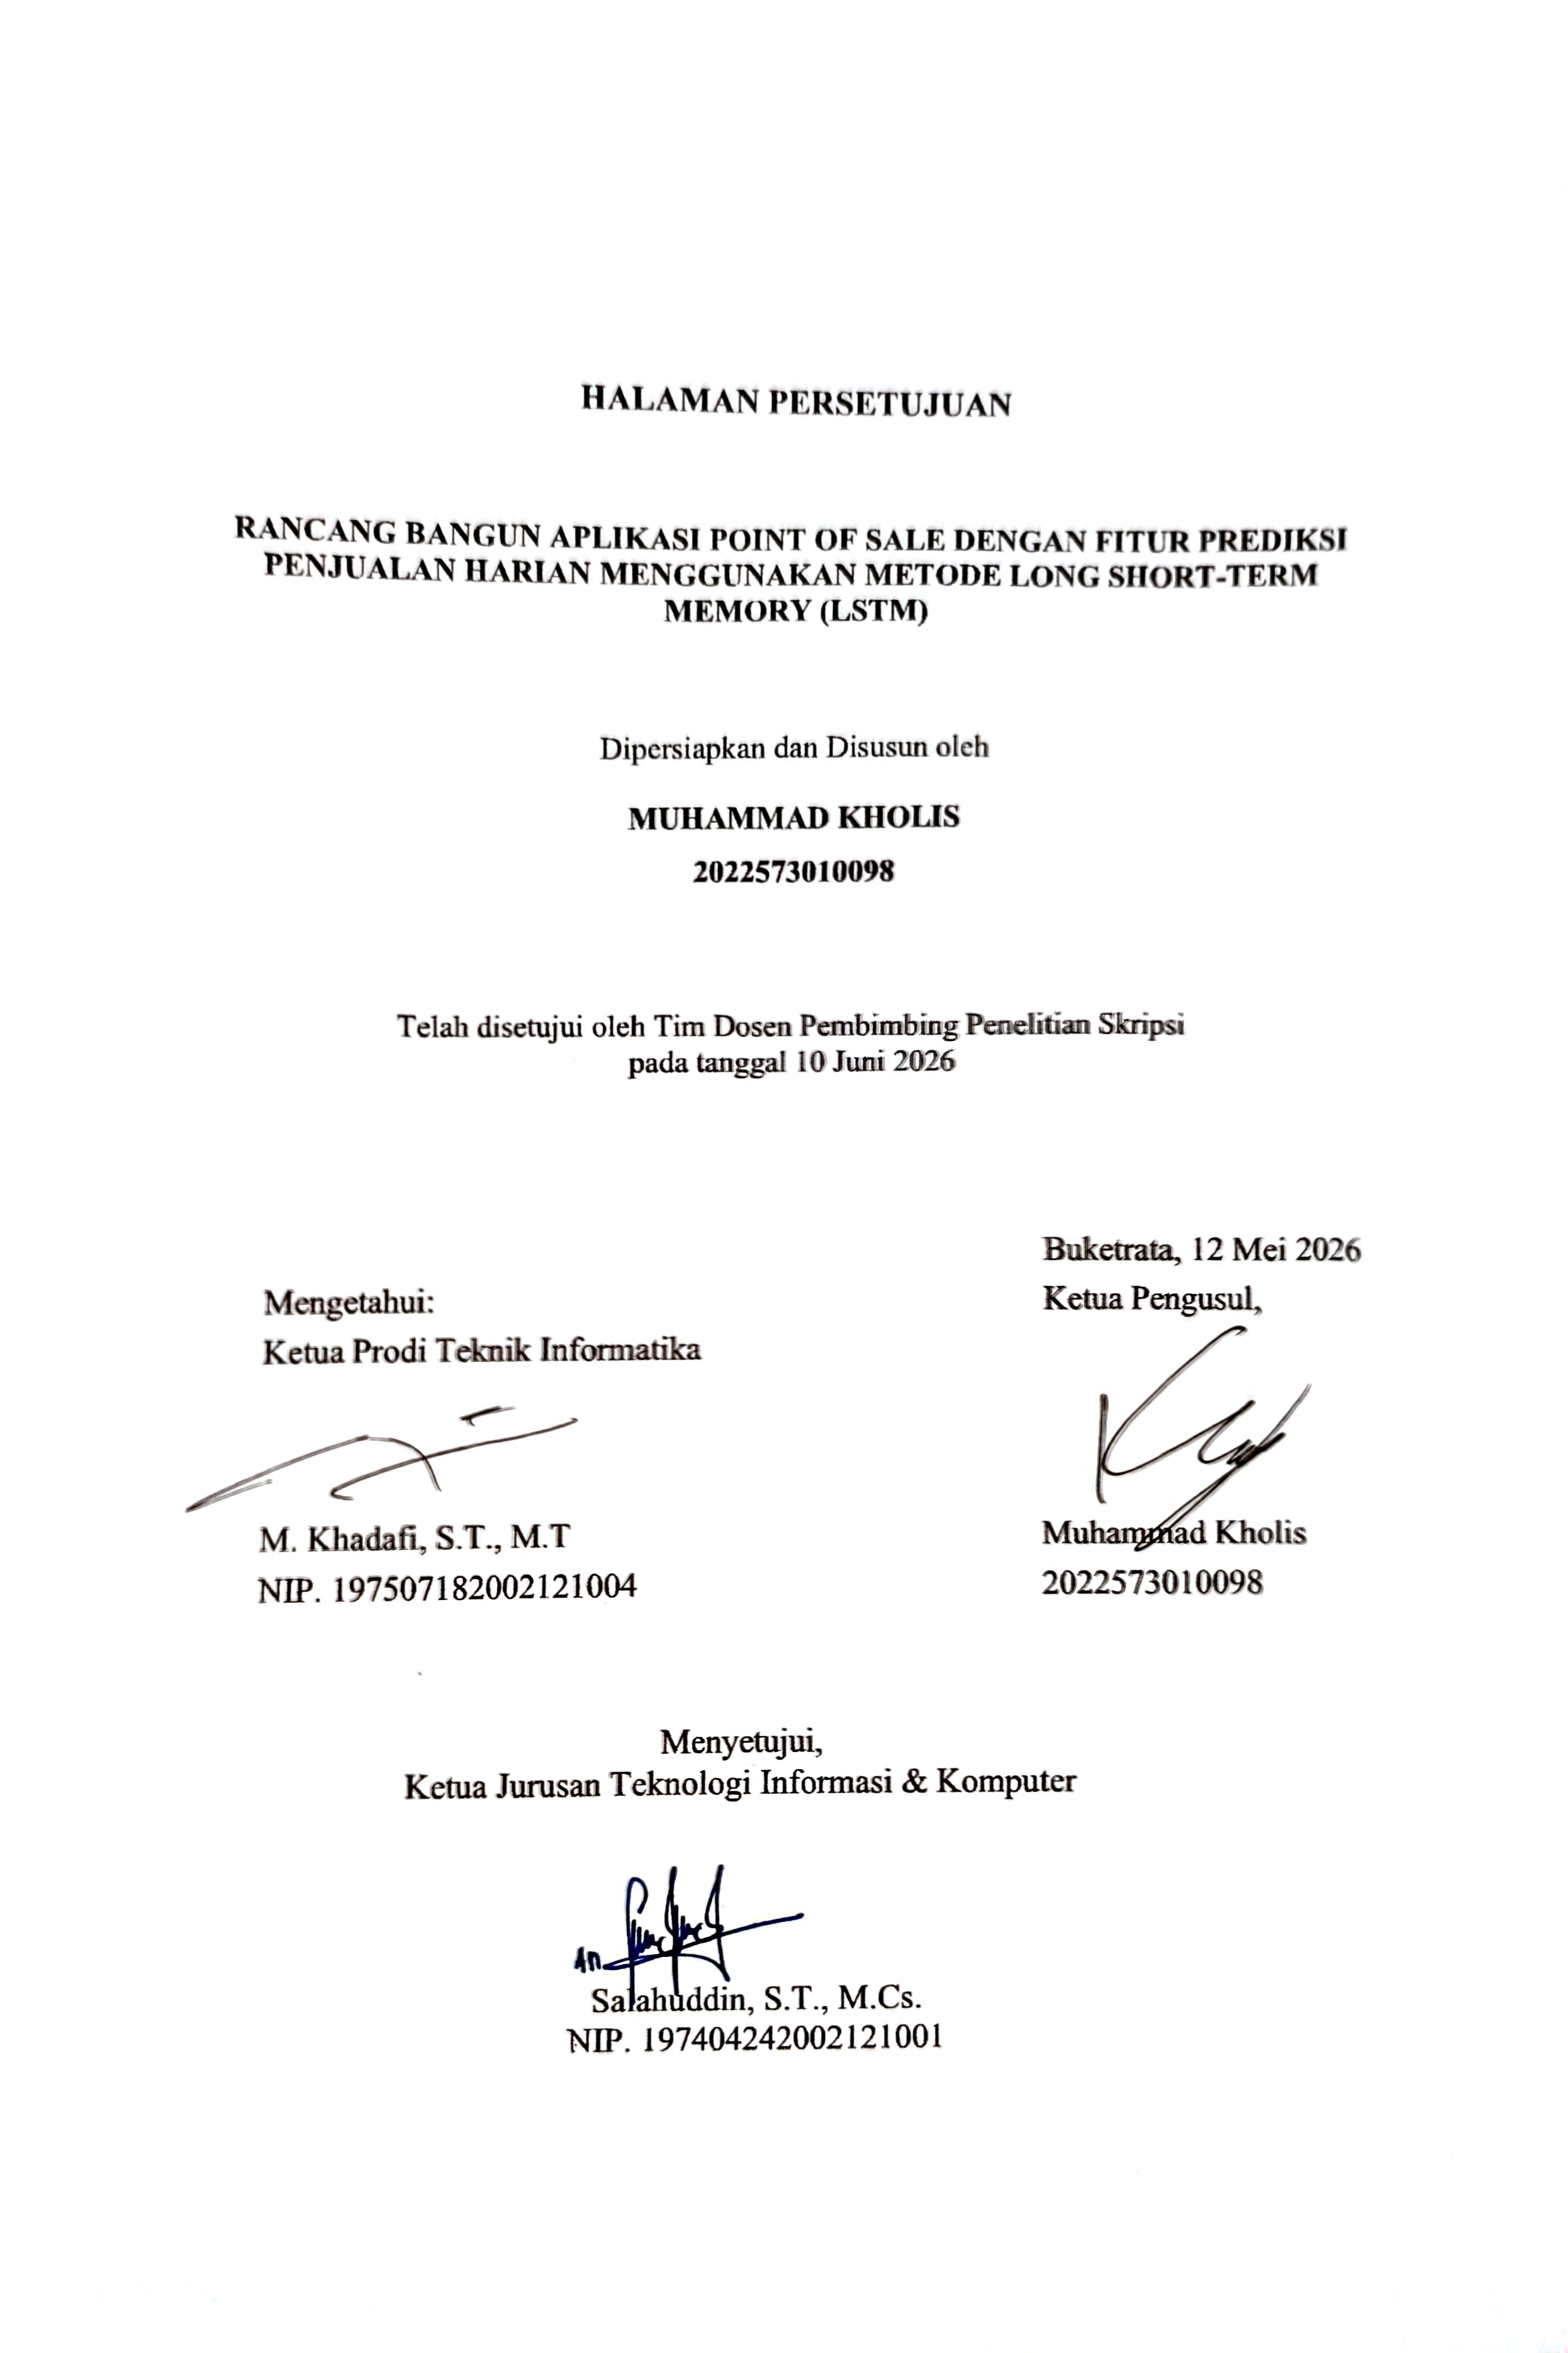
\includegraphics[width=\paperwidth,height=\paperheight]{Gambar/halaman-pengesahan}
\restoregeometry

%%-------------------------------------------------------------
%% LEMBAR PERNYATAAN KEASLIAN
%%-------------------------------------------------------------
\newpage
\thispagestyle{empty}
\begin{spacing}{1.5}
\begin{center}
{\fontsize{14pt}{16pt}\selectfont\bfseries LEMBAR PERNYATAAN KEASLIAN}
\end{center}
\vspace{0.5cm}

\noindent Saya yang bertanda tangan di bawah ini:

\begin{tabular}{@{}p{3.5cm}@{ : }l@{}}
Nama & Muhammad Kholis \\
NIM & 2022573010098 \\
Program Studi & Teknik Informatika \\
Jurusan & Teknologi Informasi dan Komputer \\
\end{tabular}

\noindent menyatakan dengan sesungguhnya bahwa skripsi yang berjudul \textit{``Rancang Bangun Aplikasi Point of Sale dengan Fitur Prediksi Penjualan Harian Menggunakan Metode Long Short-Term Memory (LSTM)''} ini merupakan hasil karya saya sendiri dan bukan merupakan plagiat dari karya orang lain. Seluruh kutipan dan rujukan yang digunakan telah saya cantumkan sumbernya sesuai dengan kaidah penulisan ilmiah yang berlaku. Apabila di kemudian hari terbukti terdapat plagiat dalam skripsi ini, saya bersedia menerima sanksi sesuai dengan peraturan yang berlaku.

\vspace{1cm}
\begin{flushright}
\begin{tabular}{@{}c@{}}
Lhokseumawe, \dotfill 2026 \\
Yang membuat pernyataan, \\[2.5cm]
\textbf{\underline{Muhammad Kholis}} \\
NIM. 2022573010098
\end{tabular}
\end{flushright}
\end{spacing}

%%-------------------------------------------------------------
%% ABSTRAK & ABSTRACT
%%-------------------------------------------------------------
\newpage
\pagenumbering{roman}
\setcounter{page}{1}
\fancyhf{}
\cfoot{\thepage}
\pagestyle{fancy}

\clearpage
\phantomsection
\addcontentsline{toc}{chapter}{ABSTRAK}
\begin{spacing}{1.0}
\begin{center}
    \textbf{ABSTRAK}\\[0.5cm]
\end{center}

Penelitian ini bertujuan merancang dan membangun aplikasi \textit{Point of Sale} (POS) berbasis \textit{mobile} dengan arsitektur \textit{offline-first} yang dilengkapi fitur prediksi penjualan harian menggunakan metode \textit{Long Short-Term Memory} (LSTM), guna membantu pelaku UMKM—dalam hal ini kantin EatsTEDI Universitas Gadjah Mada sebagai mitra penelitian—dalam pengambilan keputusan operasional berbasis data. Sistem dikembangkan menggunakan \textit{framework} Flutter yang terintegrasi dengan basis data lokal Isar DB dan basis data \textit{cloud} Supabase PostgreSQL, sedangkan modul prediksi dibangun menggunakan Python (TensorFlow dan Flask) yang di-\textit{deploy} sebagai layanan API terpisah. Data yang digunakan berupa 313 hari aktif transaksi penjualan harian yang diolah sebagai data deret waktu (\textit{time series}) dengan pendekatan target \textit{log-return}. Kinerja model LSTM dievaluasi menggunakan metrik MAE, RMSE, sMAPE, dan MASE, serta dibandingkan dengan model pembanding \textit{Naive}, \textit{Mean-7}, dan SARIMA melalui pengujian \textit{multi-seed}. Hasil evaluasi menunjukkan bahwa model LSTM \textit{Hybrid} (MAE rata-rata Rp667.718,00; MASE 1,840) belum mampu mengungguli metode \textit{Naive} (MAE Rp519.841,00; MASE 1,432) akibat keterbatasan volume data historis dan dominasi persistensi jangka pendek pada data penjualan. Eksperimen augmentasi data sintetis menggunakan TimeGAN berhasil menurunkan galat model LSTM multi-langkah secara signifikan, namun tetap belum melampaui \textit{baseline Seasonal-Naive}. Berdasarkan temuan tersebut, layanan API produksi menyajikan metode \textit{Seasonal-Naive} sebagai metode penyaji utama peramalan harian. Pengujian fungsional \textit{Black Box} terhadap 14 skenario dan pengujian \textit{White Box} terhadap fungsi kritis layanan prediksi menunjukkan tingkat keberhasilan 100\%, sehingga sistem POS \textit{offline-first} ini terbukti layak dioperasikan secara penuh dalam mendukung operasional UMKM.\\[0.6cm]

\noindent \textbf{Kata Kunci}: \textit{Point of Sale} (POS), Prediksi Penjualan Harian, \textit{Long Short-Term Memory} (LSTM), \textit{Offline-First}, TimeGAN, UMKM
\end{spacing}

\newpage
\selectlanguage{english}
\phantomsection
\addcontentsline{toc}{chapter}{ABSTRACT}
\begin{spacing}{1.0}
\begin{center}
    \textbf{\textit{ABSTRACT}}\\[0.5cm]
\end{center}

\textit{This study aims to design and develop a mobile-based Point of Sale (POS) application with an offline-first architecture, equipped with a daily sales prediction feature using the Long Short-Term Memory (LSTM) method, to assist MSMEs—in this case the EatsTEDI canteen of Universitas Gadjah Mada as the research partner—in data-driven operational decision-making. The system was developed using the Flutter framework integrated with the local Isar DB database and the Supabase PostgreSQL cloud database, while the prediction module was built using Python (TensorFlow and Flask) deployed as a separate API service. The data used consist of 313 active days of daily sales transactions processed as time-series data using a log-return target approach. The performance of the LSTM model was evaluated using the MAE, RMSE, sMAPE, and MASE metrics, and compared against the Naive, Mean-7, and SARIMA baseline models through multi-seed testing. The evaluation results show that the Hybrid LSTM model (average MAE of IDR 667,718.00; MASE of 1.840) was unable to outperform the Naive method (MAE of IDR 519,841.00; MASE of 1.432) due to the limited volume of historical data and the dominance of short-term persistence in the sales data. A synthetic data augmentation experiment using TimeGAN significantly reduced the error of the multi-step LSTM model, yet still did not surpass the Seasonal-Naive baseline. Based on these findings, the production API service presents the Seasonal-Naive method as the primary forecasting method for daily predictions. Black Box functional testing on 14 scenarios and White Box testing on the critical functions of the prediction service showed a 100\% success rate, proving that this offline-first POS system is fully viable for supporting MSME operations.}\\[0.6cm]

\noindent \textbf{\textit{Keywords}}: \textit{Point of Sale (POS), Daily Sales Prediction, Long Short-Term Memory (LSTM), Offline-First, TimeGAN, MSMEs}
\end{spacing}
\selectlanguage{indonesian}

%%-------------------------------------------------------------
%% KATA PENGANTAR
%%-------------------------------------------------------------
\newpage
\phantomsection
\addcontentsline{toc}{chapter}{KATA PENGANTAR}
\begin{center}
{\fontsize{14pt}{16pt}\selectfont\bfseries KATA PENGANTAR}
\end{center}
\vspace{0.5cm}
\begin{spacing}{1.5}
Puji syukur penulis panjatkan ke hadirat Allah SWT atas segala rahmat dan karunia-Nya sehingga penulis dapat menyelesaikan skripsi yang berjudul \textit{``Rancang Bangun Aplikasi Point of Sale dengan Fitur Prediksi Penjualan Harian Menggunakan Metode Long Short-Term Memory (LSTM)''}. Skripsi ini disusun sebagai salah satu syarat penyelesaian studi pada Program Studi Teknik Informatika, Jurusan Teknologi Informasi dan Komputer, Politeknik Negeri Lhokseumawe.

Dalam proses penyusunan skripsi ini, penulis banyak memperoleh bimbingan, arahan, dan dukungan dari berbagai pihak. Oleh karena itu, penulis mengucapkan terima kasih kepada:
\begin{enumerate}
    \item Bapak Zulfan Khairil Simbolon, S.T., M.Eng., selaku Dosen Pembimbing I yang telah memberikan bimbingan dan arahan selama penyusunan skripsi ini.
    \item Bapak Azhar, S.T., M.T., selaku Dosen Pembimbing II atas segala masukan dan koreksi yang membangun.
    \item Bapak M. Khadafi, S.T., M.T., selaku Ketua Program Studi Teknik Informatika.
    \item Pengelola platform EatsTEDI Departemen Teknik Elektro dan Informatika Universitas Gadjah Mada atas izin penggunaan data transaksi sebagai bahan penelitian.
    \item Kedua orang tua dan keluarga atas doa dan dukungan yang tiada henti, serta rekan-rekan seperjuangan yang telah membantu selama proses penelitian.
\end{enumerate}

Penulis menyadari bahwa skripsi ini masih jauh dari sempurna. Oleh karena itu, kritik dan saran yang membangun sangat penulis harapkan demi perbaikan di masa mendatang. Semoga skripsi ini bermanfaat bagi pembaca dan pengembangan ilmu pengetahuan.

\begin{flushright}
\begin{tabular}{@{}c@{}}
Lhokseumawe, Juli 2026 \\[0.2cm]
Penulis
\end{tabular}
\end{flushright}
\end{spacing}

%%-------------------------------------------------------------
%% DAFTAR ISI, DAFTAR GAMBAR, DAFTAR TABEL
%%-------------------------------------------------------------
\newpage

\renewcommand{\contentsname}{}
\renewcommand{\listfigurename}{}
\renewcommand{\listtablename}{}

\phantomsection
\addcontentsline{toc}{chapter}{DAFTAR ISI}
\vspace*{-1cm}
{\centering\fontsize{14pt}{16pt}\selectfont\bfseries DAFTAR ISI\par}
\vspace{20pt}
\begin{spacing}{1.2}
\makeatletter\@starttoc{toc}\makeatother
\end{spacing}

\newpage
\phantomsection
\addcontentsline{toc}{chapter}{DAFTAR GAMBAR}
\vspace*{-1cm}
{\centering\fontsize{14pt}{16pt}\selectfont\bfseries DAFTAR GAMBAR\par}
\vspace{20pt}
\begin{spacing}{1.2}
\makeatletter\@starttoc{lof}\makeatother
\end{spacing}

\newpage
\phantomsection
\addcontentsline{toc}{chapter}{DAFTAR TABEL}
\vspace*{-1cm}
{\centering\fontsize{14pt}{16pt}\selectfont\bfseries DAFTAR TABEL\par}
\vspace{20pt}
\begin{spacing}{1.2}
\makeatletter\@starttoc{lot}\makeatother
\end{spacing}

\newpage
\phantomsection
\addcontentsline{toc}{chapter}{DAFTAR LAMPIRAN}
\vspace*{-1cm}
{\centering\fontsize{14pt}{16pt}\selectfont\bfseries DAFTAR LAMPIRAN\par}
\vspace{20pt}
\begin{spacing}{1.5}
\noindent Lampiran 1. Form Bimbingan Skripsi (Pembimbing I) \\
Lampiran 2. Form Bimbingan Skripsi (Pembimbing II) \\
Lampiran 3. Surat Izin Penggunaan Data EatsTEDI DTEDI UGM \\
Lampiran 4. Dokumentasi Observasi dan Wawancara \\
Lampiran 5. Tangkapan Layar Implementasi Aplikasi \\
Lampiran 6. Cuplikan Dataset Transaksi
\end{spacing}

%%=============================================================
%% BAB I - PENDAHULUAN
%%=============================================================
\newpage
\pagenumbering{arabic}
\setcounter{page}{1}
\fancyhf{}
\rhead{\thepage}
\pagestyle{fancy}

\begin{spacing}{1.5}

\chapter[PENDAHULUAN]{\\ PENDAHULUAN}

\section{Latar Belakang}
Perkembangan teknologi informasi dan komunikasi telah mendorong transformasi digital di berbagai sektor bisnis, termasuk pada pengelolaan transaksi dan operasional penjualan usaha mikro, kecil, dan menengah (UMKM). Pemanfaatan sistem \textit{Point of Sale} (POS) berbasis aplikasi kini menjadi salah satu solusi yang banyak digunakan untuk membantu pelaku usaha mencatat transaksi, mengelola stok, serta menyusun laporan penjualan secara lebih terstruktur dan efisien~[1]. Namun, Pratama dan Handayani~[2] mencatat bahwa adopsi teknologi kasir digital di Indonesia masih terbatas, di mana minimnya fitur analitik menjadi penyebab utama UMKM gagal mengantisipasi siklus musiman penjualan.

Pada praktiknya, sebagian besar aplikasi POS yang digunakan UMKM masih bersifat deskriptif, yaitu hanya menampilkan data historis penjualan tanpa kemampuan analisis prediktif. Pelaku usaha umumnya harus melakukan estimasi penjualan secara manual berdasarkan pengalaman atau intuisi, sehingga rentan menimbulkan kesalahan dalam perencanaan stok, penentuan target, maupun pengelolaan arus kas. Ketidakmampuan sistem dalam memprediksi penjualan harian secara akurat dapat memicu berbagai permasalahan, seperti kelebihan stok (\textit{overstock}), kekurangan persediaan (\textit{stockout}), serta strategi penjualan yang tidak optimal~[3].

Perkembangan teknologi kecerdasan buatan, khususnya bidang \textit{deep learning}, membuka peluang untuk menghadirkan fitur prediksi penjualan yang lebih akurat dan adaptif terhadap pola data historis. Salah satu metode \textit{deep learning} yang banyak digunakan dalam analisis data runtun waktu (\textit{time series}) adalah \textit{Long Short-Term Memory} (LSTM). Abbas dkk.~[4] membuktikan bahwa LSTM mengungguli model ARIMA konvensional dalam memprediksi data penjualan ritel harian berfluktuasi non-linier tinggi, dengan penurunan \textit{error} hingga 15\%. Wilson dan Davies~[5] menjelaskan bahwa mekanisme \textit{forget gate} pada arsitektur LSTM mampu mempertahankan memori pola penjualan jangka panjang, seperti tren musiman akibat periode Ramadan atau Tahun Baru, yang sering menjadi titik kritis operasional UMKM. Choi dan Lee~[6] lebih lanjut menunjukkan bahwa penambahan variabel kontekstual seperti jumlah transaksi harian pada model LSTM \textit{multivariate} dapat meningkatkan akurasi prediksi secara signifikan.

Efektivitas penerapan model prediksi tersebut akan semakin optimal apabila didukung oleh arsitektur sistem yang andal pada kondisi lapangan UMKM. Tantangan infrastruktur menjadi hambatan nyata, khususnya koneksi internet yang tidak stabil di daerah. Martinez dan Silva~[7] menunjukkan bahwa arsitektur \textit{offline-first} dengan basis data lokal \textit{embedded} merupakan solusi efektif untuk menjamin kelancaran operasional sistem pada jaringan yang tidak andal. Novikov dan Petrov~[8] membuktikan bahwa Isar DB unggul sebagai basis data lokal pada aplikasi Flutter berkat kecepatan operasi baca-tulis yang optimal dibandingkan alternatif seperti Hive dan ObjectBox. Untuk mendukung ekosistem \textit{cloud backend} yang andal, Fischer dan Weber~[9] mengevaluasi Supabase sebagai platform \textit{Backend-as-a-Service} (BaaS) \textit{open-source} dengan fitur \textit{Row Level Security} (RLS) dan \textit{real-time subscription} yang sesuai untuk pengelolaan data transaksi multi-tenant UMKM.

Meskipun riset terdahulu telah membuktikan keunggulan masing-masing komponen secara terpisah, belum ada penelitian yang mengintegrasikan keseluruhan komponen tersebut menjadi satu sistem yang utuh. Kumar dan Sharma~[10] menyoroti tantangan latensi ketika modul AI di-\textit{deploy} sebagai layanan terpisah yang dipanggil aplikasi klien kasir. Nguyen dan Tran~[11] merekomendasikan pemisahan beban kerja transaksional dari beban kerja analitik melalui arsitektur \textit{microservices} agar sistem kasir tidak terganggu selama proses pelatihan model. Roberts dan Thomas~[12] membahas standarisasi pengiriman data dari aplikasi \textit{mobile} ke server AI berbasis \textit{REST API}, yang menjadi jembatan integrasi antara sistem POS dan modul prediksi.

Dalam konteks operasional UMKM di Lhokseumawe, kebutuhan akan sistem kasir yang tidak hanya mampu mencatat transaksi, tetapi juga memprediksi penjualan harian secara akurat sekaligus tetap berfungsi dalam kondisi jaringan terbatas menjadi semakin penting. Kompleksitas pengambilan keputusan stok dan tingginya dinamika pola penjualan menuntut solusi yang memadukan keandalan operasional \textit{offline} dengan kecerdasan analitik prediktif dalam satu kesatuan sistem.

Berdasarkan permasalahan tersebut, penelitian ini bertujuan merancang dan membangun aplikasi \textit{Point of Sale} berbasis \textit{mobile} Android dengan arsitektur \textit{offline-first} menggunakan \textit{framework} Flutter dan Isar DB, yang secara bersamaan dilengkapi fitur prediksi penjualan harian berbasis metode LSTM yang dieksekusi di sisi server melalui \textit{REST API}. Aplikasi yang dikembangkan dalam penelitian ini diberi nama \textbf{Parzello POS Mobile}, dan diharapkan mampu berfungsi sebagai \textit{Decision Support System} bagi pelaku UMKM dalam mengambil keputusan manajemen stok dan strategi penjualan secara lebih akurat dan berbasis data.

\section{Rumusan Masalah}
Berdasarkan latar belakang yang telah diuraikan, maka rumusan masalah dalam penelitian ini adalah sebagai berikut:
\begin{enumerate}
    \item Bagaimana merancang dan membangun aplikasi \textit{Point of Sale} (POS) dengan fitur prediksi penjualan harian berbasis \textit{mobile} yang dapat digunakan oleh pelaku usaha secara efektif?
    \item Bagaimana keandalan arsitektur \textit{offline-first} dalam menjamin keberlangsungan pencatatan transaksi kasir pada kondisi konektivitas internet yang tidak stabil?
    \item Bagaimana menerapkan metode \textit{Long Short-Term Memory} (LSTM) pada aplikasi \textit{Point of Sale} untuk memprediksi penjualan harian berdasarkan data transaksi historis?
    \item Bagaimana tingkat akurasi hasil prediksi penjualan harian yang dihasilkan oleh metode \textit{Long Short-Term Memory} (LSTM) berdasarkan evaluasi menggunakan metrik kesalahan prediksi?
\end{enumerate}

\section{Tujuan Penelitian}
Berdasarkan rumusan masalah yang telah diuraikan, maka tujuan dalam penelitian ini adalah sebagai berikut:
\begin{enumerate}
    \item Merancang dan membangun aplikasi \textit{Point of Sale} (POS) berbasis \textit{mobile} yang dilengkapi dengan fitur prediksi penjualan harian sebagai alat bantu pengelolaan dan analisis penjualan.
    \item Menguji keandalan arsitektur \textit{offline-first} berbasis Isar DB dan mekanisme sinkronisasi otomatis ke Supabase dalam menjaga keberlangsungan transaksi kasir pada kondisi jaringan tidak stabil.
    \item Mengimplementasikan metode \textit{Long Short-Term Memory} (LSTM) pada aplikasi \textit{Point of Sale} untuk memprediksi penjualan harian berdasarkan data transaksi historis.
    \item Mengevaluasi kinerja dan tingkat akurasi metode \textit{Long Short-Term Memory} (LSTM) dalam menghasilkan prediksi penjualan harian menggunakan metrik evaluasi kesalahan prediksi.
\end{enumerate}

\section{Batasan Masalah}
Untuk menghindari meluasnya materi pembahasan, maka penelitian ini dibatasi pada hal-hal berikut:
\begin{enumerate}
    \item Aplikasi dikembangkan menggunakan \textit{framework} Flutter dan difokuskan untuk sistem operasi Android, mengingat dominasi pasar Android pada segmen UMKM lokal.
    \item Basis data yang digunakan adalah Supabase dengan skema relasional untuk menyimpan data produk, transaksi, dan akun pengguna.
    \item Algoritma yang digunakan adalah \textit{Long Short-Term Memory} (LSTM) dengan model \textit{univariate} atau \textit{multivariate} terbatas, dan prediksi dilakukan untuk rentang waktu harian.
    \item Data uji bersumber dari basis data transaksi riil platform EatsTEDI DTEDI Universitas Gadjah Mada dengan periode lebih dari satu tahun; pola musiman yang diobservasi bersifat kalender akademis (mingguan dan semester), karena cakupan data yang tersedia belum cukup untuk mengamati siklus musiman tahunan penuh secara statistik.
    \item Proses pelatihan model dan prediksi dilakukan di sisi \textit{server/cloud} menggunakan bahasa Python, sedangkan aplikasi \textit{mobile} bertugas mengirim data transaksi dan menerima hasil prediksi melalui \textit{REST API}.
\end{enumerate}

\section{Manfaat Penelitian}
Manfaat yang diharapkan dari penelitian ini adalah sebagai berikut:
\begin{enumerate}
    \item \textbf{Bagi Pelaku UMKM}: Memberikan aplikasi \textit{Point of Sale} (POS) berbasis \textit{mobile} yang dapat digunakan untuk pencatatan transaksi penjualan dan pengelolaan stok secara digital, serta menyediakan fitur prediksi penjualan harian berbasis algoritma LSTM sebagai alat bantu dalam pengambilan keputusan \textit{restock} dan pengelolaan persediaan barang.
    \item \textbf{Bagi Akademisi}: Menjadi referensi dan bahan kajian dalam pengembangan penelitian di bidang sistem informasi dan \textit{machine learning}, khususnya penerapan metode LSTM untuk prediksi penjualan harian pada sistem POS berbasis \textit{mobile} di lingkungan UMKM.
    \item \textbf{Bagi Peneliti}: Menambah pengetahuan dan pengalaman dalam merancang dan membangun aplikasi POS berbasis \textit{mobile} menggunakan \textit{framework} Flutter serta mengimplementasikan algoritma LSTM untuk menyelesaikan permasalahan prediksi penjualan harian berbasis data transaksi UMKM pada studi kasus nyata.
\end{enumerate}

\section{Sistematika Penulisan}
Sistematika penulisan skripsi ini disusun untuk memberikan gambaran secara menyeluruh mengenai alur pembahasan yang dilakukan. Sistematika penulisan dibagi menjadi lima bab utama yang saling berkaitan, dengan rincian sebagai berikut:

\noindent\textbf{BAB I PENDAHULUAN}\\
Bab ini menguraikan gambaran umum penelitian yang meliputi latar belakang masalah, rumusan masalah, tujuan penelitian, batasan masalah, manfaat penelitian, serta sistematika penulisan. Bab ini menjadi dasar dalam memahami alasan dan arah penelitian yang dilakukan.

\noindent\textbf{BAB II TINJAUAN PUSTAKA}\\
Bab ini berisi kajian literatur dan landasan teori yang relevan dengan penelitian. Kajian mencakup perbandingan metode peramalan penjualan dan implementasi sistem POS berbasis \textit{mobile}. Landasan teori menyajikan konsep peramalan, arsitektur LSTM, \textit{framework} Flutter, bahasa Dart, serta layanan Supabase yang digunakan sebagai infrastruktur sistem.

\noindent\textbf{BAB III METODOLOGI PENELITIAN}\\
Bab ini menjelaskan tahapan metodologi penelitian yang dilakukan, meliputi jenis dan pendekatan penelitian, teknik pengumpulan data, teknik analisis data, alur penelitian, rancangan sistem menggunakan UML, teknik pengujian, serta indikator keberhasilan penelitian.

\noindent\textbf{BAB IV HASIL DAN PEMBAHASAN}\\
Bab ini menyajikan hasil implementasi sistem POS \textit{mobile} beserta layanan API prediksi, tahapan \textit{preprocessing} data, implementasi dan pelatihan model peramalan LSTM beserta eksperimen augmentasi TimeGAN, evaluasi komparatif model terhadap \textit{baseline}, hasil pengujian \textit{Black Box} dan \textit{White Box}, pembahasan temuan penelitian, serta keterbatasan sistem dan penelitian.

\noindent\textbf{BAB V KESIMPULAN DAN SARAN}\\
Bab ini memuat kesimpulan yang menjawab rumusan masalah dan tujuan penelitian berdasarkan hasil yang diperoleh, serta saran-saran konstruktif untuk pengembangan sistem dan penelitian lanjutan di masa mendatang.

%%=============================================================
%% BAB II - TINJAUAN PUSTAKA
%%=============================================================
\chapter[TINJAUAN PUSTAKA]{\\ TINJAUAN PUSTAKA}

\section{\textit{State Of The Art}}

Penelitian terkait prediksi penjualan dan pengembangan sistem \textit{Point of Sale} berbasis \textit{mobile} telah mengalami perkembangan signifikan seiring meningkatnya pemanfaatan teknologi \textit{deep learning} dan komputasi awan. Abbas dkk.~[4] dan Zhang dan Liu [13] membuktikan keunggulan LSTM dibandingkan model statistik konvensional maupun arsitektur \textit{Gated Recurrent Unit} (GRU) dalam menangkap pola non-linier pada data penjualan ritel. Choi dan Lee [6] memperluas pendekatan ini dengan menggunakan model multivariate yang menggabungkan variabel kontekstual seperti frekuensi transaksi harian. Di sisi pengembangan sistem, Setiawan dan Nugroho [1] serta Pratama dan Handayani [2] mengembangkan aplikasi POS berbasis Android untuk UMKM, namun keduanya bersifat murni deskriptif tanpa komponen prediksi analitik.

Meskipun demikian, penelitian yang secara spesifik mengintegrasikan modul prediksi penjualan berbasis LSTM langsung ke dalam sistem POS \textit{mobile} yang beroperasi secara \textit{offline-first} untuk konteks UMKM masih sangat terbatas. Ringkasan penelitian terdahulu tersebut disajikan dalam Tabel~\ref{tab:sota}.

\setlength{\tabcolsep}{4pt}
{\small\setstretch{1.1}\hyphenpenalty=50\exhyphenpenalty=50\tolerance=500
\begin{longtable}{|>{\centering\arraybackslash}p{0.6cm}|>{\raggedright\arraybackslash}p{2.2cm}|>{\raggedright\arraybackslash}p{2.2cm}|>{\raggedright\arraybackslash}p{2.2cm}|>{\raggedright\arraybackslash}p{2.2cm}|>{\raggedright\arraybackslash}p{2.8cm}|}

\caption{\textit{State Of The Art}} \label{tab:sota} \\
\hline
\textbf{No} &
\textbf{Penulis, Tahun dan Judul Artikel} &
\textbf{Metode yang Digunakan} &
\textbf{Hasil yang Diperoleh} &
\textbf{Persamaan} &
\textbf{Perbedaan} \\
\hline
\endfirsthead

\multicolumn{6}{@{}l}{Tabel \thetable\ \textit{(lanjutan)}}\\
\hline
\textbf{No} &
\textbf{Penulis, Tahun dan Judul Artikel} &
\textbf{Metode yang Digunakan} &
\textbf{Hasil yang Diperoleh} &
\textbf{Persamaan} &
\textbf{Perbedaan} \\
\hline
\endhead

\hline
\endfoot

\hline
\endlastfoot

1 &
Abbas dkk.~(2021) [4]. \textit{Sales Forecasting Using LSTM Networks in Retail Industry}. &
LSTM, ARIMA &
LSTM mengungguli ARIMA pada data penjualan non-linier dengan penurunan \textit{error} hingga 15\%. &
Sama-sama menggunakan LSTM untuk prediksi data penjualan berbasis deret waktu. &
Model bersifat \textit{standalone} tanpa integrasi sistem kasir nyata; penelitian ini mengintegrasikan LSTM ke dalam aplikasi POS. \\
\hline

2 &
Setiawan \& Nugroho (2023) [1]. \textit{Development of Cross-Platform POS Application using Flutter for SMEs}. &
Flutter, Firebase &
Aplikasi kasir stabil dan mampu mencatat transaksi secara \textit{real-time}. &
Sama-sama mengembangkan aplikasi POS berbasis Android untuk UMKM. &
Aplikasi murni deskriptif tanpa fungsi prediksi analitik; penelitian ini menambahkan modul LSTM terintegrasi. \\
\hline

3 &
Martinez \& Silva (2022) [7]. \textit{Architecture Design of Offline-First Mobile Application using Local Embedded Database}. &
\textit{Offline-First}, SQLite &
Data tersinkronisasi aman tanpa tumpang tindih saat kembali \textit{online}. &
Sama-sama menerapkan arsitektur \textit{offline-first} pada aplikasi \textit{mobile}. &
Tidak menguji volume data besar dan tidak memiliki komponen AI; penelitian ini mengintegrasikan keduanya. \\
\hline

4 &
Zhang \& Liu (2022) [13]. \textit{Comparative Analysis of LSTM and GRU for Time-Series Sales Forecasting}. &
LSTM, GRU &
LSTM memberikan akurasi lebih stabil pada data tren penjualan multi-tahun. &
Sama-sama membandingkan model \textit{deep learning} untuk prediksi deret waktu penjualan. &
Memerlukan daya komputasi tinggi; penelitian ini men-\textit{deploy} model di server \textit{cloud} terpisah agar tidak membebani perangkat. \\
\hline

5 &
Fischer \& Weber (2024) [9]. \textit{Evaluating Open-Source BaaS Platforms: A Case Study on Supabase and PostgreSQL}. &
Supabase, PostgreSQL &
RLS Supabase memangkas waktu pengembangan \textit{backend} hingga 40\%. &
Sama-sama menggunakan Supabase sebagai infrastruktur \textit{backend cloud}. &
Belum diuji untuk performa \textit{mobile dynamic sync} berskala harian; penelitian ini mengujinya dalam konteks UMKM. \\
\hline

6 &
Choi \& Lee (2022) [6]. \textit{Multivariate Time-Series Forecasting for Retail Sales Using LSTM with Economic Indicators}. &
Multivariate LSTM &
Akurasi model naik dengan menambahkan variabel kontekstual seperti hari libur. &
Sama-sama menggunakan variabel transaksi harian sebagai input model LSTM. &
Bergantung pada data eksternal yang sulit diakses pelaku UMKM kecil; penelitian ini menggunakan data transaksi internal saja. \\
\hline

7 &
Novikov \& Petrov (2023) [8]. \textit{Performance Comparison of Local NoSQL Embedded Databases in Flutter: Hive, ObjectBox, and Isar}. &
Isar DB, Hive, ObjectBox &
Isar DB tercepat dalam operasi \textit{batch insert} transaksi pada perangkat Android. &
Sama-sama menggunakan Isar DB sebagai \textit{local storage} pada aplikasi Flutter. &
Belum diintegrasikan ke arsitektur sinkronisasi \textit{cloud}; penelitian ini mengintegrasikan keduanya secara penuh. \\
\hline

8 &
Brown \& Green (2021) [3]. \textit{Demand Forecasting for Inventory Management in Small Retail Stores Using Neural Networks}. &
Neural Networks &
Mampu memprediksi \textit{demand} mingguan dengan MAPE 12\%. &
Sama-sama menghubungkan prediksi penjualan ke manajemen stok barang. &
Rentang prediksi mingguan terlalu luas; penelitian ini berfokus pada prediksi harian yang lebih granular. \\
\hline

9 &
\textbf{Penelitian Ini.} Rancang Bangun Aplikasi \textit{Point of Sale} dengan Fitur Prediksi Penjualan Harian Menggunakan Metode LSTM. &
\textbf{LSTM, Flutter, Supabase, Isar DB} &
Aplikasi POS \textit{mobile offline-first} terintegrasi dengan prediksi penjualan harian berbasis LSTM menggunakan dataset transaksi riil EatsTEDI UGM. &
-- &
-- \\

\end{longtable}
}

Berdasarkan kajian terhadap penelitian terdahulu pada Tabel~\ref{tab:sota}, dapat disimpulkan bahwa sebagian besar penelitian prediksi penjualan menggunakan LSTM masih bersifat \textit{standalone}, yakni tidak terintegrasi dengan sistem pencatatan transaksi yang aktif digunakan. Sebaliknya, penelitian pengembangan sistem POS \textit{mobile} yang ada belum dilengkapi kemampuan analitik prediktif berbasis \textit{machine learning}. Selain itu, belum ada sistem POS untuk UMKM yang secara bersamaan menerapkan arsitektur \textit{offline-first} sekaligus menyertakan modul prediksi LSTM terintegrasi.

Oleh karena itu, penelitian ini hadir untuk mengisi celah tersebut dengan mengusulkan sistem yang menggabungkan ketiga aspek sekaligus, yaitu: (1) aplikasi POS \textit{mobile} berbasis Flutter dengan kemampuan operasional \textit{offline-first} menggunakan Isar DB dan sinkronisasi otomatis ke Supabase [8], [9]; (2) modul prediksi penjualan harian berbasis LSTM yang dilatih dari data transaksi riil platform EatsTEDI DTEDI Universitas Gadjah Mada [4]--[6]; dan (3) penyajian hasil prediksi secara langsung kepada pengguna melalui dasbor analitik di dalam aplikasi yang sama [12].

\section{Sistem \textit{Point of Sale} (POS)}

Sistem \textit{Point of Sale} (POS) merupakan kombinasi perangkat keras dan perangkat lunak yang digunakan untuk memproses transaksi penjualan pada titik pembelian. Dalam konteks UMKM, sistem POS berfungsi sebagai alat pencatatan transaksi, pengelolaan stok barang, dan pelaporan keuangan yang menggantikan proses manual berbasis buku catatan. Perkembangan teknologi \textit{mobile} telah mendorong lahirnya aplikasi POS berbasis Android yang lebih fleksibel, murah, dan mudah dioperasikan oleh pelaku usaha kecil tanpa keahlian teknis khusus [1], [2].

Sistem POS modern yang dirancang untuk UMKM memerlukan pendekatan yang berbeda dibandingkan sistem ritel skala besar. Fokus utama harus terletak pada kesederhanaan alur kerja kasir, kecepatan proses transaksi, dan kemampuan beroperasi dalam kondisi konektivitas internet yang tidak stabil. Arsitektur \textit{offline-first} menjadi solusi utama untuk memastikan kelancaran operasional, di mana data transaksi disimpan terlebih dahulu secara lokal dan disinkronkan ke \textit{cloud} secara otomatis ketika koneksi tersedia [7].

\section{Peramalan Penjualan (\textit{Forecasting})}

Peramalan penjualan merupakan proyeksi teknis dari permintaan pelanggan potensial untuk periode waktu tertentu berdasarkan asumsi-asumsi yang ditetapkan. Menurut Heizer dan Render [14], peramalan yang akurat sangat krusial dalam manajemen operasi karena mempengaruhi keputusan strategis di bidang pemasaran, keuangan, dan sumber daya manusia. Terdapat empat prinsip utama dalam peramalan: peramalan jarang sekali sempurna, peramalan jangka pendek biasanya lebih akurat daripada jangka panjang, peramalan agregat lebih akurat daripada peramalan item individu, dan pemilihan metode harus disesuaikan dengan pola data (horizontal, tren, musiman, atau siklis).

Metode kuantitatif dalam peramalan mengandalkan model matematika untuk memproyeksikan data masa lalu ke masa depan. Dalam konteks ritel, tantangan utama adalah menangani variasi musiman, yaitu fluktuasi yang berulang dalam jangka waktu kurang dari satu tahun, seperti lonjakan penjualan menjelang hari raya atau awal bulan. Pendekatan berbasis \textit{deep learning}, khususnya LSTM, terbukti lebih unggul dibandingkan metode statistik konvensional seperti ARIMA dalam menangkap pola jangka panjang pada data penjualan harian yang bersifat nonlinier [4],[13]. Evaluasi akurasi model peramalan umumnya menggunakan kombinasi metrik MAE (\textit{Mean Absolute Error}), RMSE (\textit{Root Mean Square Error}), dan MAPE (\textit{Mean Absolute Percentage Error}) secara bersamaan untuk menghindari bias pembacaan akurasi akibat lonjakan data [15]. Khusus pada data yang memuat nilai aktual mendekati nol, metrik persentase simetris sMAPE dan metrik galat terskala MASE lebih dianjurkan karena tahan terhadap pembagian dengan nol [16]. Brown dan Green [3] menunjukkan bahwa prediksi berbasis jaringan saraf tiruan dapat mencapai MAPE 12\% pada data permintaan ritel kecil, sementara penggunaan pendekatan multivariate dapat meningkatkan presisi tersebut lebih jauh [6].

\section{Arsitektur \textit{Long Short-Term Memory} (LSTM)}

LSTM adalah jenis khusus dari \textit{Recurrent Neural Network} (RNN) yang pertama kali diperkenalkan oleh Hochreiter dan Schmidhuber [17] dan memiliki kemampuan untuk mempelajari ketergantungan jangka panjang dalam urutan data [4],[5]. Arsitektur LSTM dirancang untuk mengatasi masalah \textit{vanishing gradient} yang menghambat RNN standar dalam memproses informasi yang terpisah jauh dalam satu urutan [5]. Komponen inti dari unit LSTM adalah \textit{cell state} (keadaan sel) yang bertindak sebagai jalur informasi utama, serta tiga gerbang fungsional:
\begin{enumerate}
    \item \textbf{\textit{Forget Gate}:} Menggunakan fungsi aktivasi sigmoid untuk menentukan bagian informasi dari status sel sebelumnya yang harus dibuang.
    \item \textbf{\textit{Input Gate}:} Memutuskan informasi baru mana yang akan diperbarui ke dalam status sel melalui kombinasi fungsi sigmoid dan tanh.
    \item \textbf{\textit{Output Gate}:} Menentukan bagian dari status sel yang akan dikeluarkan sebagai \textit{hidden state} untuk langkah waktu berikutnya.
\end{enumerate}

Secara matematis, ketiga gerbang beserta kandidat status sel pada langkah waktu $t$ dirumuskan sebagai berikut [17]:
\begin{equation}
    f_t = \sigma(W_f \cdot [h_{t-1}, x_t] + b_f)
\end{equation}
\begin{equation}
    i_t = \sigma(W_i \cdot [h_{t-1}, x_t] + b_i)
\end{equation}
\begin{equation}
    \tilde{C}_t = \tanh(W_C \cdot [h_{t-1}, x_t] + b_C)
\end{equation}
\begin{equation}
    o_t = \sigma(W_o \cdot [h_{t-1}, x_t] + b_o)
\end{equation}

\noindent di mana $\sigma$ adalah fungsi aktivasi sigmoid, $x_t$ adalah masukan pada langkah waktu $t$, $h_{t-1}$ adalah \textit{hidden state} sebelumnya, serta $W$ dan $b$ masing-masing adalah matriks bobot dan bias tiap gerbang. Pembaruan status sel $C_t$ dan \textit{hidden state} $h_t$ kemudian dinyatakan sebagai:
\begin{equation}
    C_t = f_t \odot C_{t-1} + i_t \odot \tilde{C}_t
\end{equation}
\begin{equation}
    h_t = o_t \odot \tanh(C_t)
\end{equation}

\noindent Di mana $f_t$ adalah \textit{output} dari \textit{forget gate}, $i_t$ adalah \textit{output} dari \textit{input gate}, $o_t$ adalah \textit{output} dari \textit{output gate}, dan $\tilde{C}_t$ adalah kandidat nilai baru yang akan ditambahkan ke dalam status sel.

Dalam praktiknya, pelatihan jaringan LSTM umumnya menggunakan algoritma optimasi \textbf{Adam} (\textit{Adaptive Moment Estimation}), yaitu metode optimasi berbasis gradien stokastik yang menyesuaikan \textit{learning rate} secara adaptif untuk setiap parameter dan terbukti efisien pada berbagai permasalahan \textit{deep learning} [18]. Untuk mencegah \textit{overfitting} pada data latih berukuran kecil, diterapkan teknik regularisasi \textbf{Dropout}, yaitu menonaktifkan sebagian neuron secara acak selama pelatihan agar jaringan tidak bergantung berlebihan pada neuron tertentu [19].

\section{Model Pembanding Peramalan (\textit{Baseline})}

Dalam penelitian peramalan deret waktu, kinerja sebuah model kompleks harus selalu disandingkan dengan model pembanding sederhana (\textit{baseline}) untuk memvalidasi apakah kompleksitas tambahan benar-benar memberikan nilai tambah akurasi [20]. Beberapa \textit{baseline} standar yang digunakan dalam penelitian ini adalah:
\begin{enumerate}
    \item \textbf{\textit{Naive}}: Nilai peramalan disamakan dengan nilai observasi terakhir yang tersedia. Metode ini menjadi tolok ukur minimum yang wajib dikalahkan oleh model yang lebih kompleks [20].
    \item \textbf{\textit{Seasonal-Naive}}: Nilai peramalan diambil dari observasi terakhir pada musim yang sama — misalnya penjualan hari Senin diprediksi dari rata-rata beberapa hari Senin sebelumnya — sehingga efektif menangkap pola musiman mingguan [20].
    \item \textbf{\textit{Moving Average} (Rata-rata Bergerak)}: Nilai peramalan berupa rata-rata dari $k$ observasi terakhir, berguna untuk meredam fluktuasi acak jangka pendek [14].
    \item \textbf{SARIMA} (\textit{Seasonal Autoregressive Integrated Moving Average}): Model statistik klasik dari keluarga Box--Jenkins yang memodelkan komponen autoregresif, diferensiasi, rata-rata bergerak, beserta pola musimannya secara eksplisit [21].
\end{enumerate}

Temuan pada kompetisi peramalan berskala global M3 dan M4 menunjukkan bahwa metode statistik klasik dan kombinasinya kerap mengungguli metode \textit{machine learning} murni pada deret waktu bisnis, terutama ketika data historis yang tersedia terbatas [22],[23]. Temuan tersebut menjadi dasar metodologis dalam penelitian ini untuk mengevaluasi model LSTM secara jujur terhadap \textit{baseline} sederhana sebelum diputuskan metode mana yang layak disajikan kepada pengguna akhir.

\section{Metrik Evaluasi Peramalan (sMAPE dan MASE)}

Selain MAE dan RMSE, penelitian ini menggunakan dua metrik evaluasi tambahan yang direkomendasikan untuk deret waktu bisnis dengan skala nilai yang bervariasi [16]:
\begin{enumerate}
    \item \textbf{sMAPE} (\textit{Symmetric Mean Absolute Percentage Error}): Varian MAPE yang membagi galat absolut terhadap rata-rata nilai aktual dan prediksi, sehingga terhindar dari ledakan nilai persentase ketika nilai aktual mendekati nol dan memiliki batas atas galat sebesar 200\%.
    \item \textbf{MASE} (\textit{Mean Absolute Scaled Error}): Metrik yang diusulkan Hyndman dan Koehler [16] untuk menormalisasi galat model terhadap galat metode naif \textit{in-sample} pada data latih. Nilai MASE $< 1$ menandakan model lebih baik daripada metode naif, sehingga metrik ini dapat dibandingkan lintas dataset tanpa terpengaruh satuan nominal.
\end{enumerate}

\section{\textit{Generative Adversarial Network} (GAN) dan TimeGAN}

\textit{Generative Adversarial Network} (GAN) adalah kerangka pembelajaran generatif yang diperkenalkan oleh Goodfellow dkk.~[24], terdiri atas dua jaringan saraf yang saling berkompetisi: \textit{generator} yang berusaha menghasilkan data tiruan semirip mungkin dengan data asli, dan \textit{discriminator} yang berusaha membedakan data asli dari data tiruan. Melalui proses pelatihan \textit{adversarial} ini, \textit{generator} secara bertahap belajar mereproduksi distribusi data asli, sehingga GAN banyak dimanfaatkan untuk augmentasi data (\textit{data augmentation}) ketika jumlah data riil terbatas.

\textbf{TimeGAN} (\textit{Time-series Generative Adversarial Networks}) merupakan pengembangan GAN yang dirancang khusus untuk data deret waktu, diusulkan oleh Yoon dkk.~[25] pada konferensi NeurIPS 2019. Berbeda dengan GAN konvensional yang hanya menangkap distribusi statis, TimeGAN menggabungkan kerangka \textit{adversarial} (\textit{unsupervised}) dengan pelatihan \textit{supervised} pada ruang laten agar dinamika temporal antar-langkah waktu pada data asli ikut dipelajari. Arsitektur TimeGAN terdiri atas lima komponen jaringan: \textit{embedder} dan \textit{recovery} yang memetakan data ke/dari ruang laten (\textit{autoencoder}), serta \textit{generator}, \textit{supervisor}, dan \textit{discriminator} yang dilatih dalam tiga fase (pelatihan \textit{autoencoder}, pelatihan \textit{supervised}, dan pelatihan gabungan \textit{adversarial}) [25]. Dalam penelitian ini, TimeGAN digunakan untuk mensintesis sekuens data penjualan harian tambahan sebagai upaya mitigasi keterbatasan ukuran dataset pada pelatihan model LSTM.

\section{\textit{Framework} Flutter dan Bahasa Dart}

Flutter merupakan \textit{framework} pengembangan aplikasi \textit{cross-platform} yang dikembangkan oleh Google dan menggunakan mesin grafis Skia untuk merender antarmuka pengguna secara langsung, menghasilkan performa tinggi mendekati aplikasi \textit{native} [1]. Bahasa pemrograman Dart yang menyertai Flutter mendukung fitur \textit{Just-In-Time} (JIT) untuk pengembangan cepat dan \textit{Ahead-Of-Time} (AOT) untuk rilis produksi yang efisien. Arsitektur \textit{widget} pada Flutter memungkinkan pengembang membangun komponen antarmuka yang modular dan dapat digunakan kembali, sangat cocok untuk aplikasi POS yang memiliki banyak elemen interaktif.

Dalam penelitian ini, Flutter dipilih sebagai \textit{framework} utama pengembangan aplikasi \textit{mobile} karena kemampuannya menghasilkan aplikasi Android berkinerja tinggi dari satu basis kode, serta dukungan ekosistem \textit{package} yang kaya untuk integrasi fitur seperti koneksi Bluetooth, pemindaian barcode, dan komunikasi \textit{REST API} [1], [12].

\section{Layanan Supabase dan Integrasi \textit{Cloud}}

Supabase merupakan platform \textit{Backend-as-a-Service} (BaaS) \textit{open-source} yang menyediakan lapisan infrastruktur matang di atas basis data PostgreSQL [9]. Supabase mencakup fitur autentikasi pengguna, \textit{real-time subscriptions}, penyimpanan file, dan \textit{Row Level Security} (RLS) yang memungkinkan pengelolaan hak akses data secara granular. Fischer dan Weber [9] membuktikan bahwa penggunaan RLS pada Supabase dapat memangkas waktu pengembangan \textit{backend} hingga 40\% sekaligus mengamankan data transaksi multi-tenant. Fitur \textit{real-time subscriptions} pada Supabase memungkinkan aplikasi \textit{mobile} menerima pembaruan data secara instan tanpa perlu melakukan \textit{polling} ke server.

Penggunaan Supabase dalam penelitian ini memfasilitasi penyimpanan data transaksi terpusat dalam jumlah besar sebagai muara sinkronisasi data penjualan dari perangkat kasir. Supabase juga menangani autentikasi multi-pengguna (Owner dan Kasir) dengan mekanisme \textit{Role-Based Access Control} (RBAC) yang terimplementasi langsung di lapisan basis data, memastikan privasi data antar-merchant terjaga [26].

\section{Isar Database (\textit{Local Storage})}

Isar DB adalah basis data \textit{embedded} berkinerja tinggi yang dirancang khusus untuk Flutter dan mendukung operasi baca/tulis secara \textit{asynchronous} tanpa memerlukan koneksi internet. Novikov dan Petrov [8] membuktikan bahwa Isar DB memiliki kecepatan \textit{batch insert} dan pembacaan data sekuensial yang paling optimal dibandingkan basis data lokal lain yang umum digunakan pada Flutter, yakni Hive dan ObjectBox. Isar DB beroperasi langsung di perangkat pengguna menggunakan format penyimpanan \textit{binary} yang dioptimalkan untuk kecepatan tinggi, serta mendukung kueri kompleks dengan antarmuka yang intuitif.

Dalam penelitian ini, Isar DB berperan sebagai penyimpanan lokal utama pada perangkat \textit{mobile} untuk menjamin kelancaran operasional kasir dalam kondisi \textit{offline} [7],[8]. Seluruh transaksi yang dilakukan tanpa koneksi akan disimpan terlebih dahulu di Isar DB, kemudian disinkronkan secara otomatis ke Supabase oleh mesin \textit{SyncNotifier} ketika koneksi internet tersedia kembali.

\section{Python, TensorFlow, PyTorch, dan Flask}

Python dipilih sebagai bahasa pemrograman untuk pengembangan modul prediksi di sisi server (\textit{server-side}) karena ekosistemnya yang kaya dalam bidang \textit{machine learning} dan analisis data. \textbf{TensorFlow} [27] dengan antarmuka tingkat tinggi Keras digunakan untuk membangun, melatih, dan menyimpan model LSTM [4],[5], sedangkan \textbf{PyTorch} [28] — pustaka \textit{deep learning} imperatif dengan komputasi graf dinamis — digunakan untuk mengimplementasikan model augmentasi data sintetis TimeGAN. Proses pelatihan model dilakukan di sisi server menggunakan data transaksi historis yang telah diekstraksi, kemudian layanan prediksi di-\textit{deploy} agar dapat dipanggil oleh aplikasi \textit{mobile} melalui \textit{REST API} [12], sehingga proses komputasi berat tidak membebani perangkat pengguna. Nguyen dan Tran [11] merekomendasikan pendekatan ini dalam arsitektur \textit{microservices} untuk memastikan sistem kasir tetap stabil meskipun modul AI sedang melakukan proses pelatihan ulang di sisi server.

Layanan prediksi tersebut dibangun menggunakan \textbf{Flask}, yaitu \textit{micro-framework} web Python yang ringan dan modular untuk membangun aplikasi web dan layanan API [29]. Komunikasi antara aplikasi \textit{mobile} dan layanan prediksi mengikuti gaya arsitektur \textbf{REST} (\textit{Representational State Transfer}) yang diformulasikan oleh Fielding [30], di mana setiap sumber daya diakses melalui \textit{endpoint} HTTP yang seragam (\textit{uniform interface}) tanpa menyimpan status sesi di server (\textit{stateless}), dengan format pertukaran data JSON.

\section{Layanan Firebase}

Firebase merupakan platform pengembangan aplikasi dari Google yang menyediakan kumpulan layanan siap pakai di sisi \textit{backend} untuk aplikasi \textit{mobile} [31]. Dua layanan Firebase yang dimanfaatkan pada penelitian ini adalah \textbf{Firebase Cloud Messaging} (FCM) sebagai infrastruktur pengiriman \textit{push notification} lintas perangkat secara \textit{real-time} — dimanfaatkan untuk pemberitahuan seperti peringatan stok menipis dan \textit{broadcast} pesan antar staf toko — serta \textbf{Firebase Analytics} untuk pencatatan telemetri perilaku penggunaan aplikasi (seperti volume transaksi dan pemakaian fitur) sebagai bahan evaluasi produk [31].

\section{Metode Pengembangan Perangkat Lunak \textit{Agile}}

\textit{Agile} adalah paradigma pengembangan perangkat lunak yang menekankan iterasi pendek, penyerahan produk fungsional secara bertahap (\textit{incremental}), dan adaptasi cepat terhadap perubahan kebutuhan [32]. Pendekatan \textit{iterative and incremental} membagi pengembangan menjadi siklus-siklus kecil di mana setiap siklus menghasilkan pertambahan fungsionalitas yang dapat diuji. Selanjutnya, \textbf{\textit{Lean Software Development}} yang diadaptasi Poppendieck dari prinsip \textit{lean manufacturing} menambahkan tujuh prinsip utama, antara lain menghilangkan pemborosan (\textit{eliminate waste}), memperkuat pembelajaran, menunda keputusan hingga saat paling akhir yang bertanggung jawab, dan menyerahkan produk secepat mungkin [33]. Kombinasi pendekatan ini melandasi strategi pengembangan sistem pada penelitian ini yang memprioritaskan \textit{Minimum Viable Product} (MVP) fitur inti kasir sebelum fitur analitik lanjutan.

\section{Pemodelan Sistem (UML dan ERD)}

\textit{Unified Modeling Language} (UML) adalah bahasa pemodelan visual standar untuk menspesifikasikan, memvisualisasikan, dan mendokumentasikan artefak sistem perangkat lunak [34]. Diagram UML yang digunakan pada penelitian ini meliputi \textit{Use Case Diagram} (memetakan interaksi aktor terhadap fungsi sistem beserta relasi \textit{include}/\textit{extend}), \textit{Activity Diagram} (memvisualisasikan aliran kerja dan titik keputusan proses), \textit{Sequence Diagram} (menggambarkan urutan pertukaran pesan antar-objek berdasarkan waktu), dan \textit{Class Diagram} (menggambarkan struktur kelas beserta relasinya) [34].

Adapun \textit{Entity Relationship Diagram} (ERD) adalah model konseptual basis data yang diperkenalkan oleh Chen [35], yang merepresentasikan data sebagai entitas, atribut, dan relasi antar-entitas beserta kardinalitasnya. ERD digunakan dalam penelitian ini untuk merancang skema basis data relasional PostgreSQL di sisi \textit{cloud} beserta padanan koleksi datanya di basis data lokal Isar DB.

\section{Pengujian \textit{Black Box}}

Pengujian \textit{black box} adalah teknik pengujian perangkat lunak yang memvalidasi fungsionalitas sistem murni dari sisi masukan dan keluaran yang teramati, tanpa memeriksa struktur internal kode program [32]. Penguji menyusun skenario uji berdasarkan spesifikasi kebutuhan fungsional, kemudian membandingkan hasil aktual sistem terhadap hasil yang diharapkan. Teknik ini efektif untuk memverifikasi kesesuaian perilaku fitur aplikasi terhadap kebutuhan pengguna akhir, dan pada penelitian ini diterapkan terhadap skenario-skenario penggunaan utama aplikasi POS oleh peran Owner dan Kasir [32].

\section{Pengujian \textit{White Box}}

Pengujian \textit{white box} (disebut juga \textit{glass box testing}) adalah teknik pengujian perangkat lunak yang memverifikasi kebenaran logika internal dan struktur kode program, dengan merancang kasus uji berdasarkan jalur eksekusi (\textit{code path}), percabangan keputusan (\textit{branch}), dan kondisi logika di dalam kode [32]. Berbeda dengan \textit{black box} yang hanya mengamati kesesuaian masukan--keluaran, \textit{white box} menuntut penguji memahami implementasi kode untuk memastikan setiap jalur logika kritis pernah dieksekusi dan menghasilkan keluaran yang benar, misalnya melalui pendekatan \textit{basis path testing} yang menelusuri jalur-jalur independen pada grafik alir program [32]. Pada penelitian ini, pengujian \textit{white box} diterapkan secara terbatas (\textit{lightweight}) terhadap fungsi-fungsi kritis pada layanan API prediksi, dengan menelusuri jalur percabangan logika menggunakan data masukan yang keluarannya telah dihitung secara manual sebagai acuan kebenaran (\textit{ground truth}).

%%=============================================================
%% BAB III - METODOLOGI PENELITIAN
%%=============================================================
\chapter[METODOLOGI PENELITIAN]{\\ METODOLOGI PENELITIAN}

\section{Data dan Pengumpulan Data}

\subsection{Tempat Penelitian}

Penelitian dan pengembangan sistem \textit{Point of Sale} (POS) dengan fitur prediksi penjualan harian menggunakan metode LSTM ini dilaksanakan pada beberapa lokasi yang mendukung proses perancangan, implementasi, dan pengujian, yaitu:
\begin{enumerate}
    \item \textbf{Jurusan Teknologi Informasi dan Komputer, Politeknik Negeri Lhokseumawe:} Menjadi lokasi utama dalam perancangan arsitektur sistem, penulisan kode program (aplikasi mobile Flutter dan REST API Python), pelatihan model LSTM, serta penyusunan laporan skripsi.
    \item \textbf{Departemen Teknik Elektro dan Informatika (DTEDI), Universitas Gadjah Mada:} Sebagai penyedia dataset transaksi riil platform EatsTEDI UGM yang digunakan sebagai data latih dan data uji utama untuk mengevaluasi performa model prediksi LSTM.
    \item \textbf{Pelaku UMKM di Kota Lhokseumawe:} Sebagai konteks sasaran pengguna yang melatarbelakangi analisis kebutuhan awal aplikasi kasir. Adapun pengumpulan data empiris (observasi, wawancara, dan dataset transaksi) serta pengujian sistem dilakukan pada mitra EatsTEDI DTEDI UGM, yang karakteristik operasionalnya (usaha kuliner skala mikro) dipandang merepresentasikan kebutuhan UMKM sejenis.
\end{enumerate}

\subsection{Waktu Penelitian}

Penelitian ini dilaksanakan selama 4 (empat) bulan, terhitung mulai bulan Maret 2026 sampai dengan bulan Juni 2026. Alokasi waktu pelaksanaan untuk setiap tahapan penelitian disajikan pada Tabel~\ref{tab:jadwal_penelitian}.

\begin{table}[H]
\setstretch{1.2}
\centering
\caption{Jadwal Pelaksanaan Penelitian}
\label{tab:jadwal_penelitian}
\begin{tabularx}{\textwidth}{|c|X|c|c|c|c|}
\hline
\textbf{No} & \textbf{Kegiatan} & \textbf{Maret 2026} & \textbf{April 2026} & \textbf{Mei 2026} & \textbf{Juni 2026} \\ \hline
1 & Persiapan dan Studi Literatur & \checkmark & & & \\ \hline
2 & Pengumpulan dan Analisis Data & \checkmark & \checkmark & & \\ \hline
3 & Perancangan Sistem dan UI/UX & & \checkmark & & \\ \hline
4 & Pengembangan Aplikasi POS Mobile & & \checkmark & \checkmark & \\ \hline
5 & Pelatihan dan Optimasi Model LSTM & & & \checkmark & \\ \hline
6 & Integrasi Sistem dan Pengujian & & & \checkmark & \checkmark \\ \hline
7 & Evaluasi dan Penyusunan Laporan & & & & \checkmark \\ \hline
\end{tabularx}
\end{table}

\subsection{Alat dan Bahan}

Untuk mendukung kelancaran pelaksanaan penelitian dan pengembangan sistem POS mobile, dibutuhkan alat (perangkat keras dan perangkat lunak) serta bahan penelitian dengan rincian yang disajikan pada Tabel~\ref{tab:alat_bahan}.

{\setstretch{1.15}
\begin{xltabular}{\textwidth}{|c|p{2.8cm}|p{3.5cm}|X|}
\caption{Daftar Alat dan Bahan Penelitian} \label{tab:alat_bahan} \\
\hline
\textbf{No} & \textbf{Kategori} & \textbf{Nama Alat/Bahan} & \textbf{Spesifikasi / Deskripsi} \\ \hline
\endfirsthead

\hline
\textbf{No} & \textbf{Kategori} & \textbf{Nama Alat/Bahan} & \textbf{Spesifikasi / Deskripsi} \\ \hline
\endhead

\hline
\endfoot

\hline
\endlastfoot

1 & Perangkat Keras (\textit{Hardware}) & Laptop Acer Nitro 5 & Intel Core i5 Gen 12, RAM 16 GB, SSD 512 GB, NVIDIA GeForce RTX 3050. Digunakan sebagai perangkat utama pengembangan aplikasi dan pelatihan model. \\ \cline{2-4}
& & Smartphone Android & OS Android 11. Digunakan untuk pengujian operasional aplikasi POS secara langsung di perangkat mobile. \\ \cline{2-4}
& & Printer Thermal & Bluetooth 58mm. Digunakan untuk menguji fungsionalitas cetak struk transaksi fisik. \\ \hline
2 & Perangkat Lunak (\textit{Software}) & Windows 11 & Sistem Operasi Laptop (Home Single Language). \\ \cline{2-4}
& & VS Code \& Android Studio & \textit{Integrated Development Environment} (IDE) utama untuk penulisan kode program. \\ \cline{2-4}
& & Flutter SDK (Dart) & \textit{Framework} lintas platform untuk membangun aplikasi kasir mobile. \\ \cline{2-4}
& & Python 3.10 & Bahasa pemrograman dengan TensorFlow, Keras, PyTorch, Pandas, NumPy, Scikit-Learn, dan Flask untuk melatih model LSTM, membangun modul augmentasi data sintetis TimeGAN, dan membuat REST API prediksi. \\ \cline{2-4}
& & Supabase Cloud & Basis data \textit{cloud} terpusat (PostgreSQL) untuk sinkronisasi data transaksi. \\ \cline{2-4}
& & Isar Database & Basis data lokal terbenam (\textit{embedded}) pada perangkat Android (\textit{offline-first}). \\ \cline{2-4}
& & Firebase & Layanan Google untuk \textit{push notification} (FCM) dan telemetri (Analytics). \\ \cline{2-4}
& & Jupyter Notebook & Lingkungan \textit{pipeline} riset untuk eksplorasi data dan pelatihan model peramalan. \\ \cline{2-4}
& & Hugging Face & Platform \textit{hosting} tempat layanan API prediksi Flask di-\textit{deploy}. \\ \cline{2-4}
& & Draw.io \& Mermaid.js & Alat pemodelan sistem untuk membuat diagram UML, ERD, dan arsitektur. \\ \hline
3 & Bahan Penelitian & Dataset EatsTEDI UGM & Berkas transaksi riil platform EatsTEDI DTEDI UGM dalam format SQL dump dan CSV (periode Agustus 2024 s.d. Juni 2026). \\ \hline
\end{xltabular}
}

\subsection{Variabel Data}

Variabel penelitian yang digunakan dalam proses prediksi penjualan harian dikelompokkan menjadi tiga:
\begin{enumerate}
    \item \textbf{Variabel \textit{Input} (Fitur):} Deret waktu transaksi harian EatsTEDI yang terdiri atas \textit{log-return} pendapatan, pengodean siklik (sinus--kosinus) untuk hari, minggu, dan bulan, serta penanda biner periode Ramadan. Variabel jumlah transaksi (\textit{transactions}) dan kuantitas terjual (\textit{qty\_sold}) sengaja tidak digunakan sebagai fitur untuk menghindari kebocoran data (\textit{data leakage}), karena keduanya belum tersedia saat memprediksi hari mendatang.
    \item \textbf{Variabel \textit{Output} (Target):} Nilai prediksi \textit{log-return} pendapatan, yang direkonstruksi kembali ke nominal Rupiah sebagai acuan estimasi omzet harian dan kebutuhan stok produk.
    \item \textbf{Variabel Evaluasi:} Kinerja model diukur dengan empat metrik evaluasi (MAE, RMSE, sMAPE, dan MASE). MAPE konvensional dihindari karena menghasilkan nilai tak terhingga saat dihadapkan pada hari dengan pendapatan mendekati nol. Rincian formula masing-masing metrik dijabarkan pada Subbab 3.2.10.1.
\end{enumerate}

\subsection{Sumber Data}

Data utama yang digunakan dalam penelitian ini adalah basis data transaksi penjualan harian yang bersumber dari platform katalog menu digital interaktif \textbf{EatsTEDI} pada Departemen Teknik Elektro dan Informatika (DTEDI) Universitas Gadjah Mada (UGM). \textit{Dataset} ini berupa \textit{dump} basis data relasional dalam format SQL (\textit{eatstedi-20260621-010820.sql}) berukuran 32,15 MB dengan total sekitar 395.090 baris data.

Rentang waktu transaksi riil yang digunakan adalah dari tanggal \textbf{24 Agustus 2024 s.d. 20 Juni 2026} (mencakup periode 666 hari kalender atau sekitar 22 bulan); adapun hari aktif pertama dengan transaksi tercatat setelah penyaringan adalah \textbf{26 Agustus 2024}, sehingga Bab IV menyebut rentang efektif 26 Agustus 2024 s.d. 20 Juni 2026. Data yang diekstrak berfokus pada transaksi dengan status lunas (\textit{is\_paid = 1}) dari tabel \textit{invoices} serta rincian item produk terjual dari tabel \textit{product\_sold} yang dihubungkan dengan tabel master \textit{products} dan \textit{categories}.

Secara umum, karakteristik data deret waktu (\textit{time series}) EatsTEDI UGM memiliki pola musiman unik yang sangat dipengaruhi oleh kalender akademis kampus, antara lain:
\begin{enumerate}
    \item \textbf{Pola Mingguan (\textit{weekly profile}):} Penjualan aktif hampir 100\% terkonsentrasi pada hari kerja (Senin s.d. Jumat) dengan rata-rata 195,41 transaksi per hari aktif. Sedangkan pada hari Sabtu dan Minggu, transaksi umumnya bernilai Rp 0 karena kantin kampus tutup, dengan pengecualian sejumlah kecil transaksi insidental pada hari non-kerja.
    \item \textbf{Pola Libur Akademis (\textit{academic holiday profile}):} Pada masa libur semester mahasiswa (sepanjang bulan Januari dan Juli), transaksi bernilai Rp 0 karena aktivitas perkuliahan dan operasional kantin berhenti total.
    \item \textbf{Pola Bulan Ramadan:} Omzet harian merosot tajam secara signifikan karena penutupan atau pembatasan jam operasional kantin selama bulan puasa (misalnya total omzet Maret 2025 hanya Rp 1.427.000,00 dan Maret 2026 sebesar Rp 3.531.000,00).
\end{enumerate}

Selama periode transaksi tersebut, tercatat sebanyak \textbf{61.749 transaksi} lunas dengan total produk terjual sebanyak \textbf{150.709 unit} dan menghasilkan total akumulasi omzet sebesar \textbf{Rp 501.440.492,00}. Statistik agregat tersebut dihitung dari seluruh transaksi mentah pada rentang penuh, sebelum penyaringan kalender hari kerja diterapkan. Setelah penyaringan hanya pada hari kerja aktif (tanpa akhir pekan dan libur semester Januari/Juli), analisis model pada Bab IV menggunakan \textbf{313 hari aktif} dengan total omzet sebesar \textbf{Rp 471.200.494,00} dan rata-rata pendapatan sebesar \textbf{Rp 1.505.433,00 per hari aktif}. Selisih total omzet sebesar Rp 30.239.998,00 berasal dari transaksi insidental yang terjadi pada hari-hari di luar kalender hari kerja aktif (misalnya akhir pekan atau masa libur semester yang tetap mencatat penjualan), yang ikut tereliminasi oleh penyaringan kalender pada tahap pemodelan.

Selain statistik agregat di atas, sebaran penjualan berdasarkan kategori produk pada platform EatsTEDI disajikan pada Tabel \ref{tab:kategori_sales}.

\begin{table}[H]
\setstretch{1.2}
\centering
\caption{Sebaran Penjualan Berdasarkan Kategori Produk}
\label{tab:kategori_sales}
\begin{tabular}{|c|l|r|c|c|}
\hline
\textbf{No} & \textbf{Kategori} & \textbf{Total Penjualan (Rp)} & \textbf{Total Unit} & \textbf{Kontribusi (\%)} \\ \hline
1 & Makanan Basah & 242.770.500,00 & 82.134 & 48,42\% \\ \hline
2 & Minuman & 82.122.500,00 & 16.861 & 16,38\% \\ \hline
3 & Makanan Kering & 41.969.500,00 & 10.361 & 8,37\% \\ \hline
4 & Ice Cream & 33.802.500,00 & 10.942 & 6,74\% \\ \hline
5 & Snacks & 26.671.500,00 & 10.847 & 5,32\% \\ \hline
6 & Merch & 496.000,00 & 110 & 0,10\% \\ \hline
\end{tabular}
\end{table}

Berdasarkan sebaran tersebut, kategori \textbf{Makanan Basah} menyumbang kontribusi terbesar yakni sebesar 48,42\% dari total akumulasi omzet. Karena sifat produk makanan basah yang memiliki masa simpan sangat singkat (\textit{shelf life} pendek) dan cepat basi, ketidakpastian permintaan harian dapat berakibat langsung pada kerugian usaha akibat produk sisa yang terbuang. Oleh karena itu, peramalan penjualan harian dalam penelitian ini diprioritaskan pada kategori tersebut untuk membantu pelaku usaha dalam mengoptimalkan persediaan barang.

Adapun sepuluh produk terlaris berdasarkan kuantitas penjualan harian pada platform EatsTEDI dirinci pada Tabel \ref{tab:top_products}.

\begin{table}[H]
\setstretch{1.2}
\centering
\caption{Daftar 10 Produk Terlaris EatsTEDI UGM}
\label{tab:top_products}
\begin{tabular}{|c|l|c|r|}
\hline
\textbf{No} & \textbf{Nama Produk} & \textbf{Kuantitas Terjual (Unit)} & \textbf{Total Omzet (Rp)} \\ \hline
1 & Tahu Bakso & 23.097 & 57.742.500,00 \\ \hline
2 & Tahu Bakso Balado & 16.688 & 42.020.500,00 \\ \hline
3 & Risol Mayo \& Sosis & 8.489 & 21.717.000,00 \\ \hline
4 & Cheese/Banana Roll & 3.417 & 3.417.000,00 \\ \hline
5 & Larist Air Mineral & 3.020 & 12.080.000,00 \\ \hline
6 & Sandwich Crispy & 2.796 & 11.184.000,00 \\ \hline
7 & Piscok & 2.524 & 7.572.000,00 \\ \hline
8 & Ayam Krispi & 2.495 & 6.237.500,00 \\ \hline
9 & Nasi Rames/Uduk & 2.382 & 11.910.000,00 \\ \hline
10 & Donat & 2.233 & 5.582.500,00 \\ \hline
\end{tabular}
\end{table}

Adapun data dikumpulkan melalui tiga saluran utama:
\begin{enumerate}
    \item \textbf{Observasi dan Wawancara:} Dilakukan terhadap pengelola divisi kewirausahaan mahasiswa platform EatsTEDI di Departemen Teknik Elektro dan Informatika UGM untuk memahami alur operasional kasir fisik, pencatatan menu harian, status stok, serta tantangan dalam mengantisipasi sisa stok makanan.
    \item \textbf{Dokumentasi Transaksi:} Mengunduh dan mengekstrak basis data transaksi digital EatsTEDI dari file \textit{dump} SQL untuk tabel \textit{invoices}, \textit{product\_sold}, \textit{products}, dan \textit{categories} sebagai data latihan (\textit{training data}) dan data uji (\textit{testing data}) model prediksi LSTM.
    \item \textbf{Studi Pustaka:} Mengkaji referensi jurnal ilmiah, buku manajemen operasi (Heizer \& Render), serta dokumentasi teknis \textit{framework} Flutter, TensorFlow LSTM, dan layanan Supabase sebagai landasan implementasi.
\end{enumerate}

\subsubsection{Ekstraksi dan Agregasi Data (Format CSV)}

Proses transformasi data mentah dari basis data relasional \textit{dump} SQL menjadi berkas terstruktur siap latih disebut sebagai proses \textbf{\textit{Extract, Transform, and Load} (ETL)} atau \textbf{Ekstraksi dan Agregasi Data}. Tahapan ini dilakukan untuk mengubah granularitas data dari log transaksi individu (tingkat item terjual) menjadi deret waktu pendapatan harian, mingguan, dan bulanan yang sesuai dengan karakteristik input jaringan saraf LSTM.

Proses ekstraksi ini menghasilkan empat berkas dataset utama sebagai berikut:
\begin{enumerate}
    \item \textbf{\texttt{raw\_transactions.csv}}: Berisi log transaksi gabungan hasil \textit{join} tabel \textit{invoices}, \textit{product\_sold}, \textit{products}, dan \textit{categories}.
    \item \textbf{\texttt{daily\_sales.csv}}: Hasil agregasi harian yang menjadi dataset utama untuk model peramalan harian.
    \item \textbf{\texttt{weekly\_sales.csv}}: Hasil agregasi mingguan untuk visualisasi tren mingguan.
    \item \textbf{\texttt{monthly\_sales.csv}}: Hasil agregasi bulanan untuk analisis musiman jangka panjang.
\end{enumerate}

Struktur skema data dan deskripsi kolom dari berkas \texttt{daily\_sales.csv} sebagai dataset utama pelatihan model LSTM dirinci pada Tabel \ref{tab:daily_sales_schema}.

\begin{table}[H]
\setstretch{1.2}
\centering
\caption{Struktur Skema Dataset \texttt{daily\_sales.csv}}
\label{tab:daily_sales_schema}
\begin{tabularx}{\textwidth}{|l|l|X|}
\hline
\textbf{Nama Kolom} & \textbf{Tipe Data} & \textbf{Deskripsi} \\ \hline
\texttt{date} & Date & Tanggal transaksi (format YYYY-MM-DD). \\ \hline
\texttt{revenue} & Float & Total omzet pendapatan harian (nominal Rupiah). \\ \hline
\texttt{transactions} & Integer & Total volume transaksi/nota lunas harian. \\ \hline
\texttt{qty\_sold} & Integer & Total kuantitas unit produk terjual harian. \\ \hline
\texttt{day\_of\_week} & Integer & Indeks hari dalam minggu (0 = Senin s.d. 6 = Minggu); penyaringan hari kerja aktif (0 s.d. 4) dilakukan pada tahap pemodelan. \\ \hline
\texttt{week\_of\_year} & Integer & Nomor minggu dalam setahun berdasarkan standar ISO. \\ \hline
\texttt{month} & Integer & Nomor bulan kalender (1 s.d. 12). \\ \hline
\texttt{is\_weekend} & Integer & Penanda biner akhir pekan (1 jika Sabtu/Minggu, 0 jika lainnya). \\ \hline
\texttt{is\_holiday} & Integer & Penanda biner libur akademik (1 jika Januari/Juli, 0 jika aktif). \\ \hline
\texttt{is\_ramadan} & Integer & Penanda biner bulan Ramadan (1 jika Ramadan, 0 jika lainnya). \\ \hline
\end{tabularx}
\end{table}

Sementara itu, skema data untuk berkas agregasi mingguan \texttt{weekly\_sales.csv} dan agregasi bulanan \texttt{monthly\_sales.csv} masing-masing dijelaskan pada Tabel \ref{tab:weekly_sales_schema} dan Tabel \ref{tab:monthly_sales_schema}.

\begin{table}[H]
\setstretch{1.2}
\centering
\caption{Struktur Skema Dataset \texttt{weekly\_sales.csv}}
\label{tab:weekly_sales_schema}
\begin{tabularx}{\textwidth}{|l|l|X|}
\hline
\textbf{Nama Kolom} & \textbf{Tipe Data} & \textbf{Deskripsi} \\ \hline
\texttt{year\_week} & String & Periode tahun dan nomor minggu ISO (format YYYY-WW). \\ \hline
\texttt{week\_start} & Date & Tanggal awal hari Senin pada minggu tersebut (format YYYY-MM-DD). \\ \hline
\texttt{revenue} & Float & Total omzet pendapatan mingguan (nominal Rupiah). \\ \hline
\texttt{transactions} & Integer & Total volume transaksi/nota lunas mingguan. \\ \hline
\texttt{qty\_sold} & Integer & Total kuantitas unit produk terjual mingguan. \\ \hline
\texttt{active\_days} & Integer & Jumlah hari aktif beroperasi dalam minggu tersebut. \\ \hline
\end{tabularx}
\end{table}

\begin{table}[H]
\setstretch{1.2}
\centering
\caption{Struktur Skema Dataset \texttt{monthly\_sales.csv}}
\label{tab:monthly_sales_schema}
\begin{tabularx}{\textwidth}{|l|l|X|}
\hline
\textbf{Nama Kolom} & \textbf{Tipe Data} & \textbf{Deskripsi} \\ \hline
\texttt{year\_month} & String & Periode tahun dan bulan kalender (format YYYY-MM). \\ \hline
\texttt{revenue} & Float & Total omzet pendapatan bulanan (nominal Rupiah). \\ \hline
\texttt{transactions} & Integer & Total volume transaksi/nota lunas bulanan. \\ \hline
\texttt{qty\_sold} & Integer & Total kuantitas unit produk terjual bulanan. \\ \hline
\texttt{active\_days} & Integer & Jumlah hari aktif beroperasi dalam bulan tersebut. \\ \hline
\end{tabularx}
\end{table}

\subsection{Analisis Kebutuhan Data}

Analisis kebutuhan data dilakukan untuk mengidentifikasi karakteristik dan kebutuhan pemrosesan data agar model prediksi LSTM dan aplikasi POS dapat berintegrasi secara optimal:
\begin{enumerate}
    \item \textbf{Volume Data Minimum (\textit{Cold Start Mitigation}):} Model LSTM memerlukan data runtun waktu yang kontinu. Ditetapkan batas minimum data transaksi historis sebanyak 30 hari aktif transaksi sebelum sistem dapat melakukan estimasi prediksi harian yang andal untuk meminimalkan masalah \textit{cold start} pada merchant baru.
    \item \textbf{Pembersihan dan Imputasi Data:} Karena data mentah transaksi sering kali memiliki hari luring atau libur, diperlukan aturan pembersihan data. Hari non-aktif (Sabtu, Minggu, dan libur semester) disaring agar tidak mengacaukan analisis pola musiman bisnis harian.
    \item \textbf{Keamanan Data (Minimalisasi Data):} \textit{Payload} yang dikirimkan ke layanan REST API prediksi secara desain hanya berisi data agregat numerik penjualan (total omzet harian, kuantitas terjual, dan indeks waktu kalender) tanpa menyertakan informasi identitas pelanggan seperti nama, nomor telepon, maupun detail pembayaran spesifik, sehingga privasi pelanggan tetap terjaga.
    \item \textbf{Struktur Payload Data API:} Data runtun waktu harus dikirimkan dalam format terstruktur JSON melalui protokol HTTPS. Payload berisi larik nominal omzet harian 7 hari terakhir beserta indeks waktu kalender yang relevan.
\end{enumerate}

\subsection{Preprocessing Data}

Data transaksi yang terkumpul dari basis data EatsTEDI melalui beberapa tahap penyiapan berikut sebelum digunakan untuk pelatihan model:
\begin{enumerate}
    \item \textbf{Pembersihan dan Penyaringan Hari Aktif:} Menghapus data duplikat dan menyelaraskan format tanggal, serta menyaring hari non-aktif (Sabtu, Minggu, dan libur semester pada Januari dan Juli); pada implementasinya, penyaringan diwujudkan dengan hanya mempertahankan hari kerja aktif yang memiliki pendapatan positif (\textit{revenue} $> 0$). Penyaringan ini mencegah \textit{gap} panjang pada deret waktu yang dapat mengaburkan pola musiman harian.
    \item \textbf{Transformasi Target:} Nilai pendapatan ditransformasikan ke skala logaritma untuk menstabilkan variansi, kemudian diubah menjadi bentuk \textit{log-return} (selisih logaritmik antar hari aktif) agar model mempelajari deviasi pendapatan relatif, bukan nilai nominal mentah.
    \item \textbf{Normalisasi:} Seluruh fitur masukan diskalakan ke rentang $[0, 1]$ menggunakan \textit{Min-Max Scaling}, dengan \textit{fitting} parameter \textit{scaler} hanya pada data latih untuk mencegah kebocoran informasi (\textit{data leakage}).
    \item \textbf{Pembentukan \textit{Sequence} (\textit{Windowing}):} Data diubah ke format \textit{input}--label menggunakan \textit{sliding window} sepanjang 7 hari kerja aktif ($LOOK\_BACK = 7$) untuk memprediksi penjualan hari aktif berikutnya.
    \item \textbf{Pembagian Data (\textit{Time-Based Split}):} Dataset dibagi secara kronologis agar urutan temporal terjaga dan tidak terjadi kebocoran data masa depan ke masa lalu.
\end{enumerate}

Rincian teknis rumus \textit{log-return}, \textit{cyclical encoding}, dan arsitektur model dijabarkan secara lengkap pada Subbagian~\ref{subsec:lstm_alg}.

\section{Rancangan Sistem}

Perancangan sistem dalam penelitian ini dilakukan menggunakan pendekatan arsitektur terdistribusi dan pemodelan \textit{Unified Modeling Language} (UML) untuk memberikan gambaran yang jelas mengenai arsitektur sistem, alur proses, dan interaksi pengguna. Pemodelan rancangan sistem direpresentasikan melalui arsitektur sistem, \textit{Use Case Diagram}, \textit{Class Diagram}, \textit{Activity Diagram}, \textit{Sequence Diagram}, serta \textit{Entity Relationship Diagram} (ERD).

\subsection{Metode Penelitian}

Penelitian ini merupakan jenis penelitian pengembangan (\textit{Research and Development}) dengan pendekatan kuantitatif untuk pengujian model prediksi dan kualitatif untuk analisis kebutuhan pengguna. Model pengembangan yang digunakan adalah \textbf{\textit{Agile} (Tangkas)} dengan pendekatan kombinasi antara \textbf{\textit{Iterative} (Berulang)} dan \textbf{\textit{Incremental} (Bertahap)}, serta mengadopsi prinsip \textbf{\textit{Lean Software Development}}. Metode ini diterapkan melalui fase-fase berikut:
\begin{enumerate}
    \item \textbf{Fokus pada \textit{Minimum Viable Product} (MVP):} Pengembangan difokuskan pada penyelesaian fitur inti sistem kasir terlebih dahulu (\textit{Core POS}, autentikasi pengguna, manajemen produk, dan integrasi \textit{hardware} printer) agar produk minimal dapat segera berfungsi untuk mempercepat waktu rilis ke pasar (\textit{time-to-market}). Fitur lanjutan seperti analisis cerdas (\textit{Smart Analytics}) dan notifikasi \textit{push} direncanakan pada fase pasca-MVP.
    \item \textbf{Pengembangan Berbasis Sesi/Iterasi Pendek (\textit{sprints}):} Proses pengembangan dipecah menjadi siklus iterasi pendek dalam bentuk sesi-sesi harian terfokus. Setiap sesi ditujukan untuk menambahkan fungsionalitas baru (\textit{increment}) secara bertahap atau melakukan optimasi spesifik, seperti perbaikan antarmuka dasbor, optimasi navigasi \textit{sidebar}, dan penataan ulang modul \textit{database}.
    \item \textbf{Refaktorisasi Kode dan Adaptasi Perubahan:} Pengembangan bersifat adaptif dan responsif terhadap kendala teknis atau perubahan kebutuhan yang ditemui di tengah proses pengembangan. Siklus mencakup proses refaktorisasi kode mengikuti pembaruan standar \textit{framework} Flutter, penyelarasan skema \textit{database} (\textit{schema alignment}), optimasi sinkronisasi data lokal-\textit{cloud}, serta mitigasi kebocoran memori (\textit{memory leaks}).
    \item \textbf{Uji Coba Berulang (\textit{Iterative Testing}):} Melakukan pengujian fungsionalitas menggunakan metode \textit{Black Box Testing} secara berkala untuk setiap penambahan fitur baru untuk memastikan integritas dan stabilitas aplikasi kasir serta modul prediksi penjualan berbasis LSTM tetap terjaga.
\end{enumerate}

\subsubsection{Alur Penelitian}

Alur penelitian ini dirancang secara sistematis untuk membangun sistem \textit{Point of Sale} (POS) berbasis \textit{mobile} yang dilengkapi fitur prediksi penjualan harian menggunakan metode LSTM. Sebagaimana diilustrasikan pada Gambar \ref{fig:alur_penelitian}, tahapan penelitian dibagi menjadi dua fase utama yang saling berkaitan.

\begin{figure}[H]
    \centering
    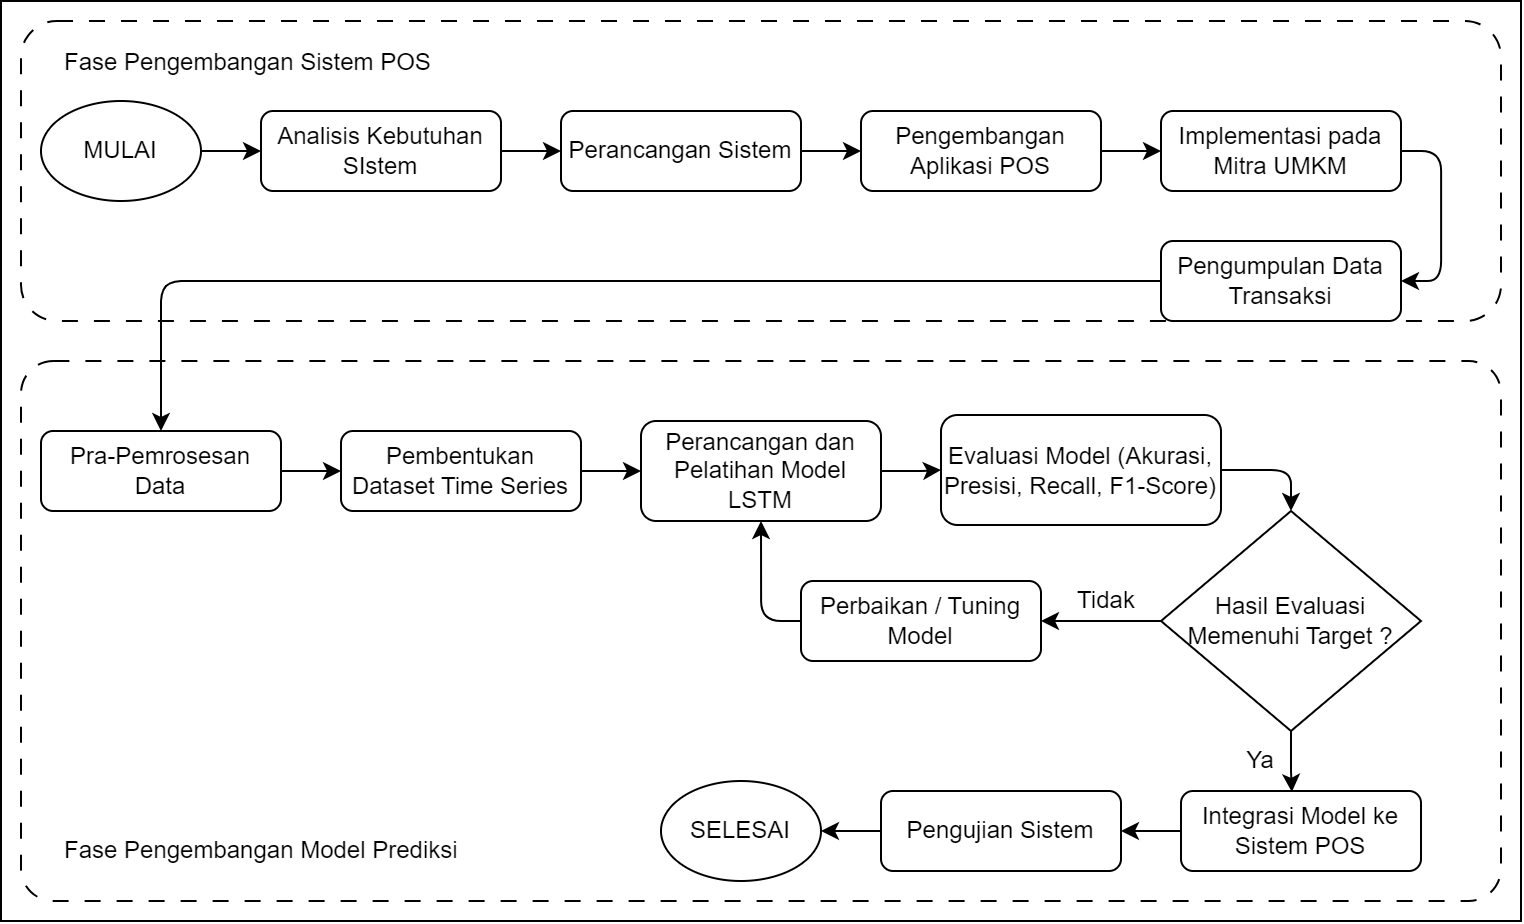
\includegraphics[width=0.85\textwidth]{alur_penelitian}
    \caption{Alur Penelitian}
    \label{fig:alur_penelitian}
\end{figure}

Pada \textbf{Fase Pengembangan dan Implementasi Sistem POS}, penelitian diawali dengan analisis kebutuhan melalui observasi langsung dan identifikasi permasalahan pada mitra EatsTEDI. Selanjutnya dilakukan perancangan sistem meliputi arsitektur \textit{offline-first}, desain basis data relasional (Supabase PostgreSQL dan Isar DB), serta perancangan \textit{Use Case Diagram}, \textit{Activity Diagram}, ERD, dan antarmuka pengguna. Setelah tahap perancangan, sistem POS dikembangkan menggunakan Flutter sebagai \textit{frontend}, Supabase sebagai basis data \textit{cloud}, Isar DB sebagai basis data lokal, dan layanan prediksi penjualan Python berbasis Flask yang di-\textit{deploy} pada platform Hugging Face untuk pengolahan modul AI. Aplikasi yang telah dibangun kemudian diimplementasikan pada mitra EatsTEDI untuk digunakan dalam kegiatan transaksi harian, sehingga menghasilkan data transaksi aktual yang tersimpan secara otomatis.

Pada \textbf{Fase Pengembangan Model Prediksi Penjualan}, data transaksi yang telah terkumpul selanjutnya melalui tahap pra-pemrosesan meliputi pembersihan data, agregasi harian, normalisasi, dan pembentukan data deret waktu (\textit{time series}). \textit{Dataset} kemudian dibagi menjadi data latih dan data uji. Model LSTM dilatih menggunakan data latih untuk mempelajari pola penjualan jangka pendek maupun jangka panjang. Setelah pelatihan, model dievaluasi menggunakan metrik regresi deret waktu, yaitu MAE, RMSE, sMAPE, dan MASE, kemudian diintegrasikan ke dalam sistem POS sehingga aplikasi mampu menampilkan hasil prediksi penjualan harian kepada pengguna melalui \textit{REST API}.

\subsection{Diagram Use Case}

Sistem POS melibatkan dua aktor utama, yaitu \textbf{Owner (Pemilik Toko)} dan \textbf{Kasir (Karyawan)}. \textit{Use Case Diagram} menggambarkan fungsi-fungsi yang dapat diakses oleh masing-masing aktor. Pembatasan hak akses berbasis peran (\textit{Role-Based Access Control}/RBAC) ditegakkan pada lapisan navigasi aplikasi (\texttt{router.dart}), di mana hanya rute Manajemen Karyawan dan Pengaturan Profil Toko yang dibatasi eksklusif untuk Owner, sedangkan fungsi operasional lainnya dapat diakses oleh seluruh staf toko. Rancangan \textit{use case} diilustrasikan pada Gambar \ref{fig:use_case}.

\begin{landscape}
\begin{figure}[p]
    \centering
    
\includegraphics[width=0.95\linewidth]{use_case_drawio}
    \caption{\textit{Use Case Diagram} Sistem POS}
    \label{fig:use_case}
\end{figure}
\end{landscape}

\noindent\textbf{1. Definisi Aktor}

Definisi aktor pada sistem POS diilustrasikan pada Tabel \ref{tab:aktor} berikut:

\begin{table}[H]
\setstretch{1.2}
\centering
\caption{Definisi Aktor}
\label{tab:aktor}
\begin{tabularx}{\textwidth}{|c|l|X|}
\hline
\textbf{No.} & \textbf{Aktor} & \textbf{Deskripsi} \\
\hline
1 & Owner (Pemilik) & Aktor dengan hak akses penuh terhadap seluruh sistem. Hak eksklusif Owner pada lapisan navigasi adalah manajemen data karyawan dan pengaturan identitas toko. Owner juga menjadi penanggung jawab utama konfigurasi toko dan pengambilan keputusan strategis berbasis laporan serta fitur AI \textit{Smart Analytics}. \\
\hline
2 & Kasir (Karyawan) & Staf operasional harian toko dengan akses mencakup pelayanan penjualan (POS), pencetakan struk, manajemen produk dan kategori, audit riwayat stok, \textit{dashboard}, laporan penjualan, \textit{broadcast} notifikasi, serta AI \textit{Smart Analytics} — kecuali manajemen karyawan dan pengaturan profil toko yang tetap eksklusif Owner. \\
\hline
\end{tabularx}
\end{table}

\noindent\textbf{2. Definisi \textit{Use Case}}

Definisi \textit{use case} pada sistem POS diilustrasikan pada Tabel \ref{tab:usecase} berikut:

{\setstretch{1.2}
\begin{longtable}{|>{\centering\arraybackslash}p{0.6cm}|>{\raggedright\arraybackslash}p{4.0cm}|>{\raggedright\arraybackslash}p{8.4cm}|}
\caption{Definisi \textit{Use Case}} \label{tab:usecase} \\
\hline
\textbf{No.} & \textbf{\textit{Use Case}} & \textbf{Deskripsi} \\
\hline
\endfirsthead
\multicolumn{3}{@{}l}{Tabel \thetable\ \textit{(lanjutan)}}\\
\hline
\textbf{No.} & \textbf{\textit{Use Case}} & \textbf{Deskripsi} \\
\hline
\endhead

\hline
\endfoot
\hline
\endlastfoot

1 & Registrasi Toko Baru & Mendaftarkan akun toko baru saat inisialisasi awal sistem (Owner). \\
\hline
2 & \textit{Login} Akun & Autentikasi pengguna menggunakan email dan kata sandi via Supabase Auth. \\
\hline
3 & Melakukan \textit{Checkout} & Memasukkan produk ke keranjang dan memproses transaksi pembayaran. \\
\hline
4 & Menerapkan \textit{Voucher}/Diskon & Memasukkan kode promosi untuk memotong total tagihan transaksi. \\
\hline
5 & Melakukan \textit{Split Bill} & Memecah pembayaran satu nota belanja menjadi beberapa bagian tagihan, terintegrasi di lembar keranjang dan layar pembayaran. \\
\hline
6 & Mencetak Struk & Mencetak struk transaksi fisik via printer \textit{thermal} Bluetooth. \\
\hline
7 & Memonitor Status Meja & Memantau keterisian meja secara visual, terintegrasi di dalam alur POS. \\
\hline
8 & Mengelola Katalog Produk & Menambah, menyunting, dan menghapus produk/stok barang. \\
\hline
9 & Mengelola Kategori & Mengatur pengelompokan menu katalog produk toko. \\
\hline
10 & Mengaudit Riwayat Stok & Melihat \textit{log} mutasi stok untuk keperluan audit inventaris. \\
\hline
11 & Melihat \textit{Dashboard} & Memantau performa keuangan dan statistik penjualan toko. \\
\hline
12 & Melihat AI \textit{Smart Analytics} & Mengakses proyeksi penjualan berbasis Model LSTM beserta riwayat hasil analitik sebelumnya. \\
\hline
13 & Kirim \textit{Broadcast} Notifikasi & Mengirim pemberitahuan \textit{real-time} ke staf toko. \\
\hline
14 & Sinkronisasi Data & Menyinkronkan transaksi \textit{offline} lokal ke \textit{cloud} Supabase secara otomatis. \\
\hline
15 & Mengelola Karyawan & Mendaftarkan atau mengubah peran staf kasir (Owner). \\
\hline
16 & Mengatur Profil Toko & Mengubah nama toko, alamat, dan logo outlet (Owner). \\
\hline
\end{longtable}
}

\subsection{Arsitektur Sistem}

Sistem Parzello POS Mobile dirancang menggunakan pendekatan arsitektur \textit{hybrid-cloud} yang membagi pemrosesan antara perangkat lokal dan infrastruktur \textit{cloud}. Secara keseluruhan, sistem terdiri dari empat komponen utama yang saling terintegrasi, yaitu \textit{Flutter Mobile App}, \textit{Supabase Cloud}, \textit{Firebase}, dan \textit{Layanan Inferensi Model LSTM} (Hugging Face). Rancangan arsitektur sistem diilustrasikan pada Gambar \ref{fig:arsitektur_sistem}.

\begin{figure}[H]
    \centering
    
\includegraphics[width=0.85\textwidth]{arsitektur_sistem}
    \caption{Arsitektur Sistem POS}
    \label{fig:arsitektur_sistem}
\end{figure}

Penjelasan mengenai empat komponen utama dalam arsitektur sistem adalah sebagai berikut:
\begin{enumerate}
    \item \textbf{Sisi Klien (\textit{Client-Side}):} Aplikasi dibangun menggunakan \textit{framework} Flutter dengan manajemen \textit{state} Riverpod dan navigasi GoRouter. Komponen inti dari sisi klien adalah Isar DB, sebuah database NoSQL lokal yang berperan sebagai \textit{cache offline-first}, memungkinkan kasir tetap dapat melakukan transaksi penuh meskipun koneksi internet terputus. \textit{Sync Engine} kemudian bekerja di latar belakang untuk menyinkronkan data lokal ke \textit{cloud} secara otomatis ketika koneksi terdeteksi kembali aktif, menggunakan penanda \texttt{isSynced} pada setiap \textit{record} untuk menghindari duplikasi data. Selain itu, sisi klien juga mengelola integrasi perangkat keras berupa printer \textit{thermal} Bluetooth/USB untuk mencetak struk dan kamera untuk pemindaian \textit{barcode} produk.
    \item \textbf{Infrastruktur \textit{Cloud} (Supabase):} Sebagai tulang punggung infrastruktur \textit{cloud}, Supabase menyediakan empat layanan utama. Supabase Auth menangani autentikasi pengguna melalui protokol JWT dan Google OAuth. Supabase PostgreSQL menjadi basis data relasional terpusat yang dilengkapi kebijakan \textit{Row Level Security} (RLS) untuk mengisolasi data antar \textit{merchant}, pemicu database (\textit{triggers}), serta prosedur tersimpan (\textit{RPC}) untuk memproses transaksi secara aman. Supabase Storage menyimpan aset media seperti gambar produk dan logo toko. Sedangkan \textit{Edge Functions} digunakan untuk memproses \textit{webhook} basis data yang bersifat sensitif, seperti pemicu pengiriman \textit{push notification} peringatan stok menipis kepada pemilik toko.
    \item \textbf{Telemetri dan Notifikasi (Firebase):} Untuk kebutuhan telemetri dan notifikasi, sistem terintegrasi dengan Firebase. \textit{Firebase Cloud Messaging} (FCM) bertugas menyampaikan \textit{push notification} secara \textit{real-time} kepada pemilik toko, misalnya peringatan stok habis atau pembatalan transaksi oleh kasir. \textit{Firebase Analytics} digunakan untuk mencatat perilaku penggunaan aplikasi, seperti volume transaksi harian, penggunaan fitur \textit{split bill}, dan inisiasi kalibrasi model AI.
    \item \textbf{Layanan Inferensi Model LSTM (Hugging Face):} Komponen terakhir adalah layanan inferensi untuk mendukung fitur analitik prediktif. Pada penelitian ini, dikembangkan sebuah model \textit{deep learning} berbasis \textbf{Long Short-Term Memory (LSTM)} secara mandiri, yang dirancang khusus untuk memproyeksikan data runtun waktu (\textit{time-series}) penjualan harian pada usaha berskala UMKM. Model peramalan tersebut kemudian dikemas dalam layanan prediksi penjualan berbasis \textit{REST API} (\textit{framework} Flask) yang di-\textit{deploy} pada platform Hugging Face, sehingga dapat diakses oleh sistem secara efisien tanpa memerlukan infrastruktur \textit{server} komputasi tersendiri. Ketika pengguna mengakses fitur \textit{Smart Analytics}, aplikasi Flutter memanggil \textit{endpoint} layanan prediksi tersebut secara langsung melalui protokol HTTPS (dikonfigurasi pada berkas \texttt{env.dart} dan dapat dioverride saat \textit{build} melalui \texttt{--dart-define}), dengan \textit{payload} berupa data agregat penjualan tanpa informasi identitas pelanggan. Model memproses data tersebut dan mengembalikan hasil prediksi dalam format JSON, mencakup estimasi omzet harian, prediksi produk terlaris, serta rekomendasi promosi berbasis stok, yang selanjutnya divisualisasikan melalui antarmuka grafik interaktif menggunakan pustaka \texttt{fl\_chart}. Aplikasi juga menangani kondisi \textit{cold start}, yaitu menampilkan peringatan pemuatan ketika \textit{server} inferensi baru aktif kembali dari kondisi \textit{idle}. Setiap hasil analisis disimpan sebagai \textit{snapshot} pada tabel \textit{smart\_analytics\_snapshots} di Supabase, sehingga riwayat analitik dapat ditinjau kembali tanpa perlu memanggil ulang model.
\end{enumerate}

\subsection{Class Diagram}

\textit{Class Diagram} menggambarkan struktur sistem dari segi pendefinisian kelas-kelas yang akan dibangun beserta atribut dan metodenya, serta hubungan relasi asosiasi antar-kelas. Pada aplikasi Parzello POS Mobile, rancangan kelas didasarkan pada koleksi basis data lokal Isar DB yang digunakan untuk mendukung penyimpanan \textit{offline-first}. Struktur kelas-kelas ini disajikan pada Gambar~\ref{fig:class_diagram}.

\begin{figure}[H]
    \centering
    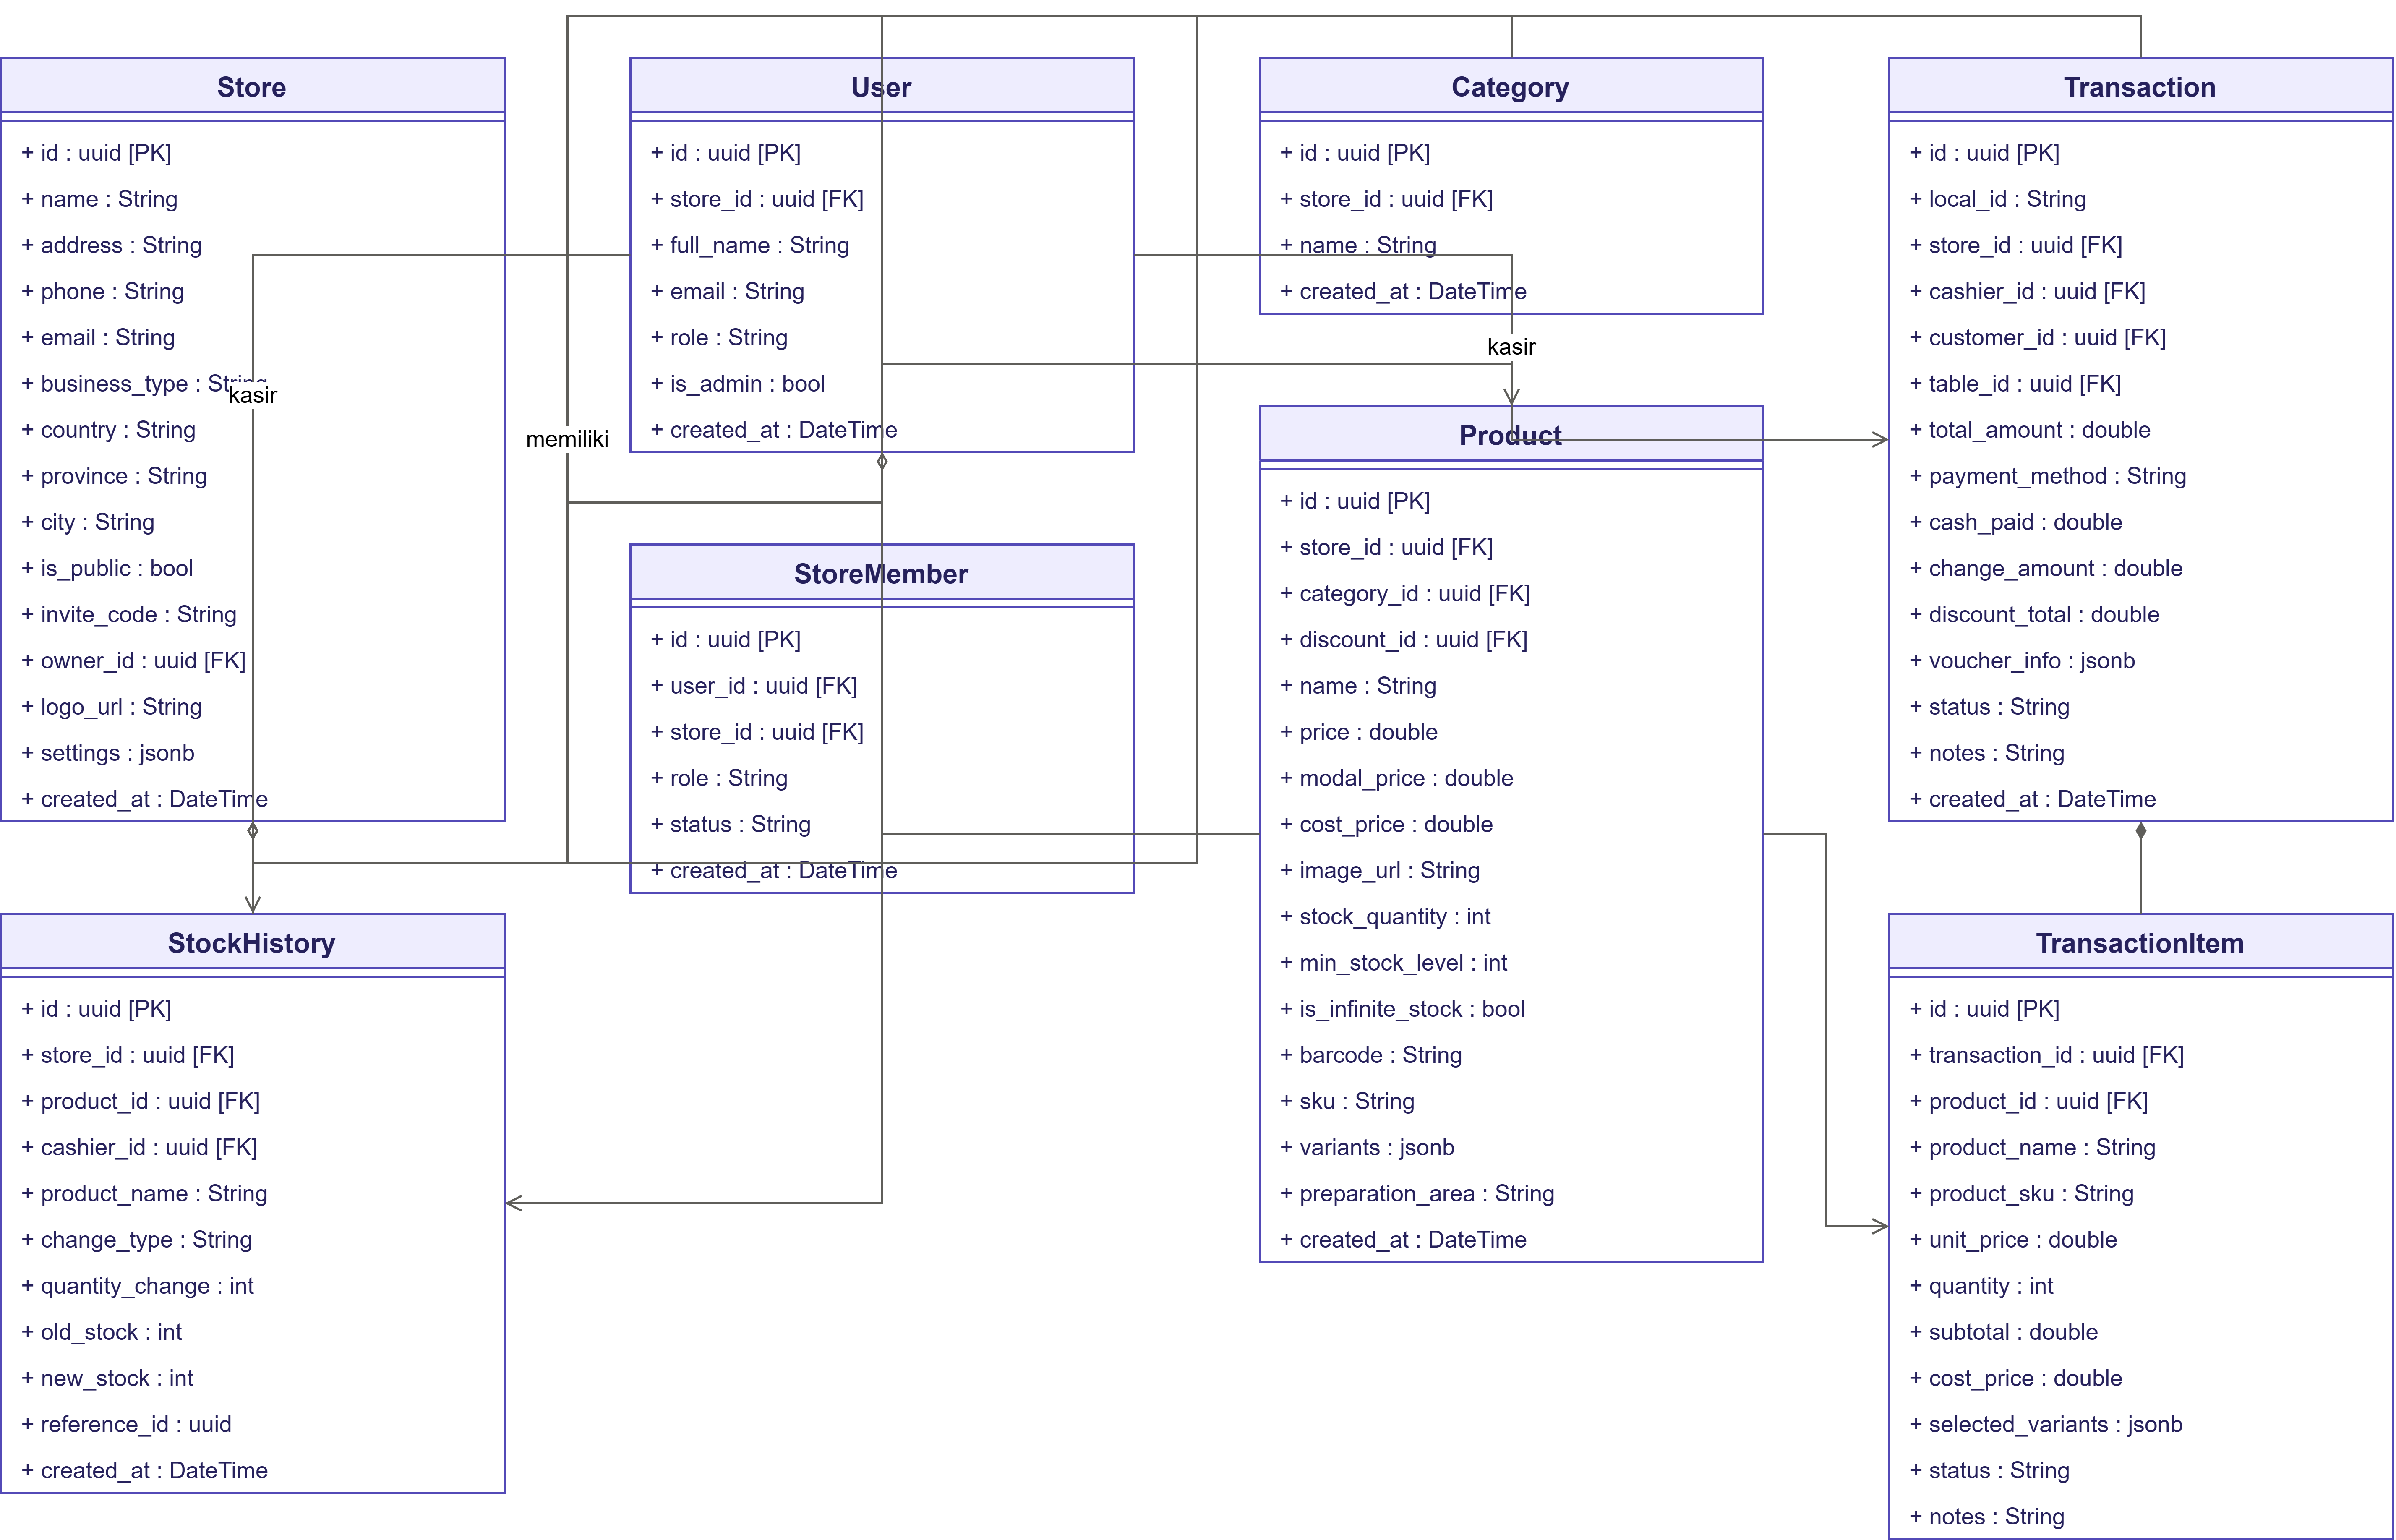
\includegraphics[width=0.92\textwidth]{../Rancangan/Class Diagram/Class Diagram.drawio.png}
    \caption{Class Diagram Sistem POS}
    \label{fig:class_diagram}
\end{figure}

Penjelasan mengenai kelas-kelas utama dalam sistem adalah sebagai berikut:
\begin{enumerate}
    \item \textbf{Store}: Merepresentasikan informasi toko/outlet, memiliki relasi satu-ke-banyak dengan Kategori, Produk, dan Transaksi.
    \item \textbf{Category}: Mengelompokkan produk ke dalam kategori tertentu.
    \item \textbf{Product}: Menyimpan informasi detail produk termasuk nama, harga jual, harga modal, dan stok.
    \item \textbf{TransactionLocal}: Menyimpan rangkuman transaksi penjualan kasir di perangkat klien.
    \item \textbf{TransactionItemLocal}: Menyimpan baris item produk detail dari setiap transaksi belanja.
\end{enumerate}

\subsection{Activity Diagram}

\textit{Activity Diagram} merupakan gambaran visual dalam bentuk diagram yang digunakan untuk menggambarkan serangkaian aktivitas atau proses yang terjadi di dalam sistem. Diagram ini memudahkan dalam menjelaskan logika prosedural, proses bisnis, serta alur kerja sistem Parzello POS Mobile yang dilengkapi dengan fitur prediksi penjualan harian. Adapun \textit{Activity Diagram} pada sistem ini dijelaskan sebagai berikut.

\begin{enumerate}
    \item \textbf{Activity Diagram Alur Kerja Transaksi Kasir (POS Checkout)} \\
    Gambar \ref{fig:act-checkout} menggambarkan alur kerja kasir atau \textit{owner} dalam memproses transaksi belanja pelanggan di kasir, termasuk opsi penerapan kupon/voucher diskon dan pemisahan tagihan (\textit{split bill}) yang terintegrasi langsung di dalam lembar keranjang belanja dan layar pembayaran, sebelum data disimpan di penyimpanan lokal Isar DB.
    
% TODO (dilengkapi sebelum sidang): re-ekspor Rancangan/Activity Diagram.md bagian 1
% (kini format mxGraphModel) melalui draw.io menjadi Rancangan/Mermaid/activity_checkout.png
    \begin{figure}[H]
        \centering
        
\includegraphics[width=0.65\textwidth,height=0.45\textheight,keepaspectratio]{activity_checkout.png}
        \caption{Activity Diagram Alur Kerja Transaksi Kasir}
        \label{fig:act-checkout}
    \end{figure}

    \item \textbf{Activity Diagram Sinkronisasi Latar Belakang (Offline-First Sync Engine)} \\
    Gambar \ref{fig:act-sync} menggambarkan logika sinkronisasi data dari \textit{local database} (Isar DB) ke cloud database (Supabase) secara otomatis saat status konektivitas terdeteksi \textit{online}. Alur data dilakukan berdasarkan ketergantungan relasi tabel (kategori, produk, transaksi, riwayat stok) untuk menjaga konsistensi, di mana pengunggahan transaksi dilakukan melalui pemanggilan prosedur RPC \texttt{create\_transaction\_v4} pada PostgreSQL agar pencatatan nota dan pemotongan stok di \textit{cloud} berlangsung dalam satu transaksi basis data yang aman.
    
% TODO (dilengkapi sebelum sidang): re-ekspor Rancangan/Activity Diagram.md bagian 2
% (kini format mxGraphModel) melalui draw.io menjadi Rancangan/Mermaid/activity_sync.png
    \begin{figure}[H]
        \centering
        
\includegraphics[width=0.65\textwidth,height=0.45\textheight,keepaspectratio]{activity_sync.png}
        \caption{Activity Diagram Sinkronisasi Latar Belakang}
        \label{fig:act-sync}
    \end{figure}

    \item \textbf{Activity Diagram Proses AI Smart Analytics} \\
    Gambar \ref{fig:act-ai} menggambarkan alur kerja fitur analitik prediktif: pengguna membuka layar \textit{Smart Analytics}, sistem mengagregasi data penjualan historis dari Isar DB lokal, lalu memanggil \textit{endpoint} model LSTM yang di-\textit{hosting} di Hugging Face secara langsung melalui HTTPS. Selama pemrosesan, sistem menampilkan status pemuatan (termasuk peringatan \textit{cold start} bila \textit{server} inferensi baru aktif dari kondisi \textit{idle}), kemudian merender visualisasi analitik omzet beserta rekomendasi promosi, dan menyimpan hasilnya sebagai \textit{snapshot} riwayat analitik di tabel \textit{smart\_analytics\_snapshots}.
    
% TODO (dilengkapi sebelum sidang): activity_ai.png SAAT INI MASIH ALUR LAMA
% (Gemini/PII scrubbing/consent modal) -- sudah TIDAK sesuai teks & kode.
% Re-ekspor Rancangan/Activity Diagram.md bagian 3 (mxGraphModel, alur baru
% panggilan langsung ke model LSTM Hugging Face) melalui draw.io menjadi
% Rancangan/Mermaid/activity_ai.png sebelum sidang.
    \begin{figure}[H]
        \centering
        
\includegraphics[width=0.65\textwidth,height=0.45\textheight,keepaspectratio]{activity_ai.png}
        \caption{Activity Diagram Proses AI Smart Analytics}
        \label{fig:act-ai}
    \end{figure}

    \item \textbf{Activity Diagram Kelola Produk (Tambah/Ubah/Hapus)} \\
    Gambar \ref{fig:act-produk} menggambarkan alur kerja staf toko dalam mengelola katalog produk yang menjadi sumber data transaksi bagi model peramalan penjualan. Proses tambah/ubah data disimpan terlebih dahulu ke basis data lokal Isar DB (\textit{offline-first}) beserta pencatatan riwayat perubahan stok, sebelum disinkronkan ke Supabase saat koneksi \textit{online} tersedia. Proses hapus produk diterapkan melalui skema \textit{soft delete} lokal (penanda \texttt{isDeleted=true}) yang baru dihapus permanen dari basis data setelah sinkronisasi ke \textit{cloud} berhasil, guna menjaga konsistensi data penjualan yang menjadi masukan pemodelan LSTM.

% TODO (dilengkapi sebelum sidang): ekspor Rancangan/Activity Diagram.md bagian 4
% (XML mxGraphModel) melalui draw.io menjadi Rancangan/Mermaid/activity_produk.png
    \begin{figure}[H]
        \centering
        
\includegraphics[width=0.65\textwidth,height=0.45\textheight,keepaspectratio]{activity_produk.png}
        \caption{Activity Diagram Kelola Produk (Tambah/Ubah/Hapus)}
        \label{fig:act-produk}
    \end{figure}
\end{enumerate}

\subsection{Sequence Diagram}

\textit{Sequence Diagram} menggambarkan interaksi dinamis antar-objek dalam sistem berdasarkan urutan waktu kejadian. Diagram ini digunakan untuk memvisualisasikan alur pesan (\textit{messages}) yang dikirim dan diterima antar-komponen saat menjalankan fungsi utama. Alur interaksi transaksi kasir pada aplikasi Parzello POS diilustrasikan pada Gambar~\ref{fig:sequence_diagram}.

\begin{figure}[H]
    \centering
    \resizebox{\textwidth}{!}{%
    \begin{tikzpicture}[
        every node/.style={font=\small},
        actor/.style={draw, rectangle, fill=white, minimum width=2cm, minimum height=0.8cm},
        lifeline/.style={draw, dashed},
        message/.style={->, >=Stealth, thick},
        reply/.style={->, >=Stealth, dashed, thick}
    ]
    % Lifelines
    \node (Kasir) [actor] {Kasir (User)};
    \node (App) [actor, right=2.5cm of Kasir] {POS App};
    \node (Isar) [actor, right=2.5cm of App] {Isar DB};
    \node (Supa) [actor, right=2.5cm of Isar] {Supabase};

    \draw [lifeline] (Kasir.south) -- +(0,-5.5) coordinate (Kasir_bottom);
    \draw [lifeline] (App.south) -- +(0,-5.5) coordinate (App_bottom);
    \draw [lifeline] (Isar.south) -- +(0,-5.5) coordinate (Isar_bottom);
    \draw [lifeline] (Supa.south) -- +(0,-5.5) coordinate (Supa_bottom);

    % Interactions
    \draw [message] (Kasir.south |- 0,-1.0) -- (App.south |- 0,-1.0) node[midway, above] {1. inputTransaksi()};
    \draw [message] (App.south |- 0,-1.8) -- (Isar.south |- 0,-1.8) node[midway, above] {2. writeTransaction(isSynced=false)};
    \draw [reply] (Isar.south |- 0,-2.4) -- (App.south |- 0,-2.4) node[midway, above] {3. writeSuccess()};
    \draw [message] (App.south |- 0,-3.0) -- (Isar.south |- 0,-3.0) node[midway, above] {4. updateStockLokal()};
    \draw [reply] (App.south |- 0,-3.6) -- (Kasir.south |- 0,-3.6) node[midway, above] {5. showCheckoutSuccess()};
    \draw [message] (App.south |- 0,-4.4) -- (Supa.south |- 0,-4.4) node[midway, above] {6. syncTransaction() (Auto-Sync)};
    \draw [reply] (Supa.south |- 0,-5.0) -- (Isar.south |- 0,-5.0) node[midway, above] {7. update isSynced=true};

    \end{tikzpicture}%
    }
    \caption{Sequence Diagram Alur Transaksi Kasir}
    \label{fig:sequence_diagram}
\end{figure}

Penjelasan alur urutan transaksi pada diagram di atas adalah sebagai berikut:
\begin{enumerate}
    \item Kasir memasukkan transaksi penjualan melalui antarmuka aplikasi POS (\texttt{inputTransaksi()}).
    \item Aplikasi menyimpan data transaksi secara lokal ke dalam Isar DB dengan status belum tersinkronisasi (\texttt{writeTransaction(isSynced=false)}).
    \item Isar DB mengembalikan respon sukses penulisan data transaksi.
    \item Aplikasi melakukan pembaruan stok produk secara lokal pada Isar DB.
    \item Aplikasi menampilkan informasi checkout sukses ke layar kasir.
    \item \textit{Sync Engine} mendeteksi status internet aktif dan menyinkronkan transaksi ke cloud Supabase melalui pemanggilan RPC \texttt{create\_transaction\_v4}.
    \item Supabase mengembalikan respon sukses, lalu \textit{Sync Engine} memperbarui status transaksi lokal menjadi \texttt{isSynced=true}.
\end{enumerate}

\subsection{\textit{Entity Relationship Diagram} (ERD)}

Basis data sistem POS dirancang secara hibrida menggunakan Supabase PostgreSQL untuk penyimpanan \textit{cloud} dan Isar DB untuk penyimpanan lokal di perangkat \textit{mobile}. Skema basis data \textit{cloud} terdiri dari sembilan entitas utama yang saling berelasi sebagaimana diilustrasikan pada Gambar \ref{fig:erd}.
\begin{landscape}
\begin{figure}[p]
    \centering
    
\includegraphics[width=1.0\linewidth, height=0.92\textheight, keepaspectratio]{erd_new}
    \caption{\textit{Entity Relationship Diagram} (ERD) Sistem POS}
    \label{fig:erd}
\end{figure}
\end{landscape}

Entitas \textit{stores} menjadi entitas induk yang berelasi dengan seluruh entitas lainnya. Entitas \textit{store\_members} mengelola hak akses berbasis peran (\textit{Role-Based Access Control}/RBAC) untuk Owner dan Kasir. Katalog produk dikelola melalui entitas \textit{products} dan \textit{categories}, sedangkan data transaksi disimpan pada entitas \textit{transactions} dan \textit{transaction\_items}. Riwayat perubahan stok dicatat pada entitas \textit{stock\_history}, sementara entitas \textit{notifications} mendukung sistem notifikasi. Adapun hasil analisis fitur AI \textit{Smart Analytics} disimpan sebagai riwayat \textit{snapshot} pada entitas \textit{smart\_analytics\_snapshots}. Daftar seluruh tabel basis data yang digunakan dirangkum pada Tabel \ref{tab:database}.

\begin{table}[H]
\setstretch{1.2}
\centering
\caption{Daftar Tabel Basis Data POS}
\label{tab:database}
\begin{tabularx}{\textwidth}{|c|l|X|}
\hline
\textbf{No.} & \textbf{Nama Tabel} & \textbf{Deskripsi} \\
\hline
1 & \textit{stores} & Menyimpan data identitas dan konfigurasi outlet toko \textit{merchant}. \\
\hline
2 & \textit{store\_members} & Mengelola hak akses dan peran staf (Owner/Kasir) pada setiap toko. \\
\hline
3 & \textit{categories} & Menyimpan kategori pengelompokan produk atau menu dagangan. \\
\hline
4 & \textit{products} & Menyimpan katalog produk beserta harga, stok, dan data SKU/\textit{barcode}. \\
\hline
5 & \textit{transactions} & Menyimpan data nota transaksi penjualan kasir sebagai tabel induk. \\
\hline
6 & \textit{transaction\_items} & Menyimpan rincian produk yang dibeli dalam setiap transaksi. \\
\hline
7 & \textit{stock\_history} & Mencatat \textit{log} audit perubahan stok masuk dan keluar produk. \\
\hline
8 & \textit{notifications} & Menyimpan pesan notifikasi sistem dan \textit{broadcast} antar staf toko. \\
\hline
9 & \textit{smart\_analytics\_snapshots} & Menyimpan riwayat \textit{snapshot} hasil analitik prediksi LSTM setiap kali fitur \textit{Smart Analytics} dijalankan. \\
\hline
\end{tabularx}
\end{table}

\subsection{Rancangan Algoritma \textit{Long Short-Term Memory} (LSTM)}
\label{subsec:lstm_alg}

Desain metode LSTM memberikan gambaran mengenai alur kerja algoritma yang digunakan dalam proses prediksi penjualan harian pada sistem POS. Alur kerja algoritma diilustrasikan pada Gambar \ref{fig:lstm_alur}.

\begin{figure}[H]
    \centering
    \resizebox{0.92\textwidth}{!}{%
    \begin{tikzpicture}[
        node distance=0.6cm,
        every node/.style={align=center},
        startstop/.style={
            rectangle, rounded corners=8pt,
            minimum width=9cm, minimum height=1cm,
            text centered, draw=black, fill=gray!20, font=\small
        },
        process/.style={
            rectangle,
            minimum width=9cm, minimum height=1cm,
            text centered, draw=black, fill=white, font=\small
        },
        decision/.style={
            diamond, aspect=2.8,
            text centered, draw=black, fill=white, font=\small,
            inner sep=3pt
        },
        arr/.style={->, >=Stealth, thick},
    ]

    \node (data)   [startstop] {Data Transaksi Harian (Supabase)};
    \node (pre)    [process, below=of data]   {Pra-pemrosesan: Filtering Hari Non-Aktif, \\ \textit{Log-Return Target}, \& Normalisasi \textit{Scaling}};
    \node (window) [process, below=of pre]    {Pembentukan \textit{Time Series} ($LOOK\_BACK=7$ hari aktif)};
    \node (split)  [process, below=of window] {Pembagian Dataset Kronologis (70\% \textit{Train}, 15\% \textit{Val}, 15\% \textit{Test})};
    \node (build)  [process, below=of split]  {Pembangunan Arsitektur LSTM Tersederhanakan\\(1 LSTM Layer 24 Units $\to$ Dropout $\to$ Dense)};
    \node (timegan) [process, minimum width=4.6cm, right=2.0cm of split]
                   {Augmentasi Data Sintetis\\TimeGAN\\(Skenario Eksperimen)};
    \node (train)  [process, below=of build]  {Pelatihan Model (Adam $5 \times 10^{-4}$, Early Stopping)};
    \node (eval)   [process, below=of train]  {Evaluasi Model: MAE, RMSE, sMAPE, MASE\\(Evaluasi \textit{Multi-Seed} \& Baseline)};
    \node (dec)    [decision, below=0.8cm of eval] {Akurasi\\Memenuhi\\Kriteria?};
    \node (tune)   [process, minimum width=3.8cm, right=2.8cm of dec]
                   {\textit{Hyperparameter Tuning}\\(\textit{epoch}, \textit{batch size},\\neuron, \textit{learning rate})};
    \node (api)    [process, below=0.8cm of dec]  {Integrasi Model ke Sistem POS via \textit{REST API}};
    \node (end)    [startstop, below=of api]  {Prediksi Harian \& Prakiraan Rekursif 7 Hari\\Ditampilkan kepada Pengguna};

    \draw [arr] (data)   -- (pre);
    \draw [arr] (pre)    -- (window);
    \draw [arr] (window) -- (split);
    \draw [arr] (split)  -- (build);
    \draw [arr] (build)  -- (train);
    \draw [arr] (train)  -- (eval);
    \draw [arr] (eval)   -- (dec);
    \draw [arr] (dec)    -- node[left,  font=\small] {Ya}    (api);
    \draw [arr] (dec)    -- node[above, font=\small] {Tidak} (tune);
    \draw [arr] (tune.north) |- (train.east);
    \draw [arr] (api)    -- (end);
    \draw [arr, dashed] (split) -- (timegan);
    \draw [arr, dashed] (timegan.south) |- (build.east);

    \end{tikzpicture}%
    }
    \caption{Alur Kerja Algoritma \textit{Long Short-Term Memory} (LSTM)}
    \label{fig:lstm_alur}
\end{figure}

Gambar \ref{fig:lstm_alur} menggambarkan alur kerja model LSTM dari \textit{input} data transaksi harian hingga proses evaluasi model. Adapun penjelasan rinci mengenai tahapan algoritma LSTM yang dirancang dalam penelitian ini adalah sebagai berikut:
\begin{enumerate}
    \item \textbf{Pra-pemrosesan Data dan Transformasi Target:}
    Data transaksi harian ditarik dari database cloud Supabase. Langkah-langkah pra-pemrosesan yang dilakukan meliputi:
    \begin{itemize}
        \item \textit{Filtering hari non-aktif (Zero Days)}: Menghapus hari Sabtu, Minggu, serta bulan Januari dan Juli (libur semester kampus) untuk menghindari distorsi gap yang panjang pada deret waktu. Model dilatih murni menggunakan indeks hari kerja aktif (\textit{business days}).
        \item \textit{Transformasi Logaritma}: Data nominal pendapatan $Y_t$ ditransformasikan ke skala logaritma menggunakan $Y'_t = \log(Y_t + 1)$ untuk menstabilkan variansi.
        \item \textit{Transformasi Target (Log-Return)}: Model tidak memprediksi pendapatan logaritmik secara langsung, melainkan memprediksi perubahan pendapatan relatif (\textit{log-return}) $r_t$ yang dirumuskan sebagai:
        \begin{equation}
            r_t = Y'_t - Y'_{t-1} = \log(Y_t + 1) - \log(Y_{t-1} + 1)
        \end{equation}
        Pendekatan \textit{hybrid residual} ini bertujuan agar model mewarisi sifat autokorelasi jangka pendek yang dominan pada data penjualan.
        \item \textit{Pengodean Siklik}: Fitur waktu (\textit{day of week}, \textit{week of year}, \textit{month}) diubah menjadi nilai sinus dan kosinus untuk merepresentasikan sifat periodik kalender.
        \item \textit{Normalisasi}: Fitur-fitur masukan dinormalisasi menggunakan \textit{Min-Max Scaling} ke rentang $[0, 1]$, di mana proses pemasangan (\textit{fitting}) parameter \textit{scaler} hanya dilakukan pada data latih (\textit{training set}) untuk mencegah kebocoran informasi (\textit{data leakage}).
    \end{itemize}

    \item \textbf{Pembentukan Sequence (Sliding Window):}
    Dataset deret waktu diubah menjadi bentuk urutan berpasangan (\textit{sequence pairs}) menggunakan metode \textit{sliding window}. Ukuran \textit{window} masukan (\textit{look-back}) ditetapkan sebesar 7 hari aktif terakhir ($LOOK\_BACK = 7$) untuk memprediksi target 1 hari aktif berikutnya ($HORIZON = 1$). Dengan demikian, model dilatih dengan format peramalan satu langkah ke depan (\textit{one-step-ahead prediction}).

    \item \textbf{Pembagian Dataset Kronologis:}
    Dataset dibagi secara kronologis (\textit{time-based split}) untuk menjaga integritas temporal deret waktu, dengan proporsi pembagian sebagai berikut:
    \begin{itemize}
        \item \textit{Data Latih (Training Set)}: Sebesar 70\% dari total data aktif (periode Agustus 2024 s.d. Agustus 2025).
        \item \textit{Data Validasi (Validation Set)}: Sebesar 15\% (periode September s.d. Desember 2025) digunakan untuk pemantauan proses latih dan \textit{early stopping}.
        \item \textit{Data Uji (Testing Set)}: Sebesar 15\% (efektif periode Februari s.d. Juni 2026, karena Januari tersaring sebagai libur semester) digunakan untuk pengujian akhir model.
    \end{itemize}

    \item \textbf{Pembangunan Arsitektur LSTM Tersederhanakan:}
    Untuk menghindari masalah \textit{overfitting} dan \textit{model collapse} pada dataset yang relatif kecil, arsitektur LSTM dirancang secara minimalis (\textit{shallow network}):
    \begin{itemize}
        \item \textit{Input Layer}: Menerima matriks berukuran $7 \times 8$ (panjang \textit{sequence} 7 dan total 8 fitur masukan).
        \item \textit{LSTM Layer}: Terdiri atas 1 \textit{layer} LSTM dengan 24 \textit{hidden units}.
        \item \textit{Dropout Layer}: Dengan laju 0,1 untuk mencegah ketergantungan berlebih antar-node.
        \item \textit{Dense Layer}: Terdiri atas 16 neuron dengan fungsi aktivasi \textit{Rectified Linear Unit} (ReLU).
        \item \textit{Output Layer}: Terdiri atas 1 neuron (\textit{Dense} dengan aktivasi linear) untuk memprediksi nilai \textit{log-return} $\hat{r}_t$.
    \end{itemize}
    Model ini memiliki total parameter terlatih sebanyak 3.585 parameter, yang sebanding dengan ukuran data latih.

    \item \textbf{Pelatihan Model:}
    Model dilatih menggunakan algoritma optimasi Adam dengan \textit{learning rate} awal sebesar $5 \times 10^{-4}$ dan fungsi kerugian (\textit{loss function}) \textit{Mean Squared Error} (MSE). Untuk mengoptimalkan konvergensi, diterapkan dua mekanisme \textit{callback}:
    \begin{itemize}
        \item \textit{Early Stopping}: Menghentikan pelatihan jika loss validasi tidak membaik selama 20 \textit{epoch} berturut-turut untuk mencegah \textit{overfitting}, serta mengembalikan bobot terbaik (\textit{restore best weights}).
        \item \textit{Reduce Learning Rate on Plateau}: Mengurangi \textit{learning rate} sebesar faktor 0,5 jika loss validasi mendatar selama 8 \textit{epoch}.
    \end{itemize}
    Ukuran \textit{batch} pelatihan diatur sebesar 16 dengan jumlah maksimum pelatihan 200 \textit{epoch}.

    \item \textbf{Evaluasi Komparatif dan Multi-Seed:}
    Untuk membuktikan keandalan model LSTM, kinerjanya dibandingkan dengan empat model pembanding (\textit{baseline}):
    \begin{itemize}
        \item \textit{Naive (Kemarin)}: Prediksi hari ini dianggap sama dengan nilai penjualan riil hari aktif sebelumnya.
        \item \textit{Mean-7}: Prediksi berupa rata-rata bergerak dari 7 hari aktif terakhir.
        \item \textit{SARIMA}: Model statistik klasik Seasonal Autoregressive Integrated Moving Average untuk mendeteksi pola autokorelasi deret waktu.
        \item \textit{Seasonal-Naive}: Prediksi berupa rata-rata beberapa kemunculan terakhir dari hari yang sama dalam minggu (Senin dengan Senin, Selasa dengan Selasa, dan seterusnya), untuk menangkap pola musiman mingguan.
    \end{itemize}
    Dari keempat \textit{baseline} tersebut, \textit{Naive}, \textit{Mean-7}, dan SARIMA dievaluasi pada skema satu langkah ke depan (\textit{one-step-ahead}), sedangkan \textit{Seasonal-Naive} dievaluasi pada skema peramalan multi-langkah dan menjadi kandidat metode penyaji pada layanan API produksi. Notasi parameter \textit{Seasonal-Naive} dilambangkan dengan $k$, yaitu jumlah kemunculan terakhir hari sejenis yang dirata-ratakan. Selain peramalan harian sebagai fokus evaluasi ilmiah, layanan API produksi juga menyajikan angka proyeksi mingguan dan bulanan menggunakan metode rata-rata sederhana (\textit{Mean-4} untuk empat minggu terakhir dan \textit{Mean-3} untuk tiga bulan terakhir); keduanya merupakan fitur pelengkap visualisasi aplikasi di luar lingkup evaluasi ilmiah penelitian ini, sejalan dengan Batasan Masalah yang memfokuskan prediksi pada rentang harian.

    Mengingat inisialisasi bobot awal jaringan saraf bersifat acak dan dapat memengaruhi stabilitas pada data kecil, evaluasi dilakukan menggunakan metode \textbf{\textit{Multi-Seed Evaluation}}. Model dilatih sebanyak 10 kali menggunakan \textit{seed} acak yang berbeda. Hasil evaluasi dilaporkan dalam bentuk rata-rata $\pm$ standar deviasi dari metrik MAE, RMSE, sMAPE, dan MASE guna memperoleh estimasi performa yang kokoh dan dapat dipertanggungjawabkan.

    \item \textbf{Eksperimen Augmentasi Data Sintetis (TimeGAN):}
    Sebagai upaya mitigasi terhadap keterbatasan jumlah data latih, dirancang skenario eksperimen augmentasi data sintetis menggunakan \textbf{TimeGAN} (\textit{Time-series Generative Adversarial Networks}), yaitu arsitektur GAN khusus deret waktu yang diusulkan oleh Yoon et al. (2019). TimeGAN diimplementasikan menggunakan \textit{framework} PyTorch dan terdiri atas lima jaringan saraf (\textit{embedder}, \textit{recovery}, \textit{generator}, \textit{supervisor}, dan \textit{discriminator}) yang dilatih dalam tiga fase: (1) pelatihan \textit{autoencoder} (embedder--recovery), (2) pelatihan \textit{supervised} pada ruang laten, dan (3) pelatihan gabungan (\textit{joint training}) secara \textit{adversarial}. Model dilatih pada jendela deret waktu sepanjang 24 hari aktif dengan tiga fitur numerik (omzet, jumlah transaksi, dan kuantitas terjual), kemudian menghasilkan 200 sekuens data harian sintetis. Data sintetis tersebut digabungkan dengan data riil untuk melatih ulang model LSTM (skenario \textit{augmented}), lalu performanya dibandingkan terhadap model LSTM tanpa augmentasi dan \textit{baseline} \textit{Seasonal-Naive} guna mengukur seberapa besar augmentasi data mampu memperbaiki akurasi peramalan pada data terbatas.

    \item \textbf{Rekonstruksi dan Prakiraan Rekursif Multi-Langkah:}
    Output model berupa \textit{log-return} prediksi ($\hat{r}_t$) direkonstruksi kembali ke skala nominal Rupiah ($\hat{Y}_t$) menggunakan nilai penjualan hari sebelumnya ($Y_{t-1}$):
    \begin{equation}
        \hat{Y}_{t} = \exp(\log(Y_{t-1} + 1) + \hat{r}_{t}) - 1
    \end{equation}
    Untuk menyajikan proyeksi 7 hari aktif ke depan pada aplikasi POS, diterapkan metode \textbf{\textit{Recursive Forecasting}} (memasukkan hasil prediksi langkah sebelumnya sebagai input untuk langkah berikutnya). Untuk mencegah masalah akumulasi bias (\textit{error propagation}) yang dapat menyebabkan nilai prediksi meluruh atau meledak, diimplementasikan tiga teknik pengaman:
    \begin{itemize}
        \item \textit{Clipping log-return}: Membatasi nilai prediksi \textit{log-return} pada rentang persentil 10--90 dari data pelatihan untuk mencegah nilai ekstrem.
        \item \textit{Damping factor}: Meredam prediksi perubahan \textit{log-return} pada langkah ke-$h$ menuju nilai 0 dengan faktor peredam $\phi^h$ (di mana $\phi = 0.7$). Hal ini membuat ramalan jangka panjang stabil dan kembali ke nilai rata-rata historis (sifat \textit{mean-reverting}).
        \item \textit{Safety rail}: Membatasi hasil akhir nominal pendapatan berada dalam rentang pendapatan terkecil dan terbesar yang pernah tercatat secara historis pada hari aktif.
    \end{itemize}
\end{enumerate}
\subsection{Perancangan \textit{Wireframe}}

Perancangan \textit{wireframe} dalam penelitian ini mencakup rancangan antarmuka pengguna untuk semua layar utama yang menjadi bagian dari alur operasional aplikasi POS. \textit{Wireframe} dirancang dengan mempertimbangkan kebutuhan pengguna, aksesibilitas, dan alur kerja yang efisien. Terdapat 13 rancangan layar yang melayani kebutuhan berbeda sesuai dengan peran pengguna, sebagaimana diuraikan berikut ini.

\begin{enumerate}

    \item \textbf{Halaman Registrasi Toko Baru}

    Halaman pendaftaran akun dan toko baru yang digunakan saat inisialisasi awal sistem oleh Owner, mencakup pengisian data identitas pengguna dan informasi outlet toko.

    \begin{figure}[H]
        \centering
        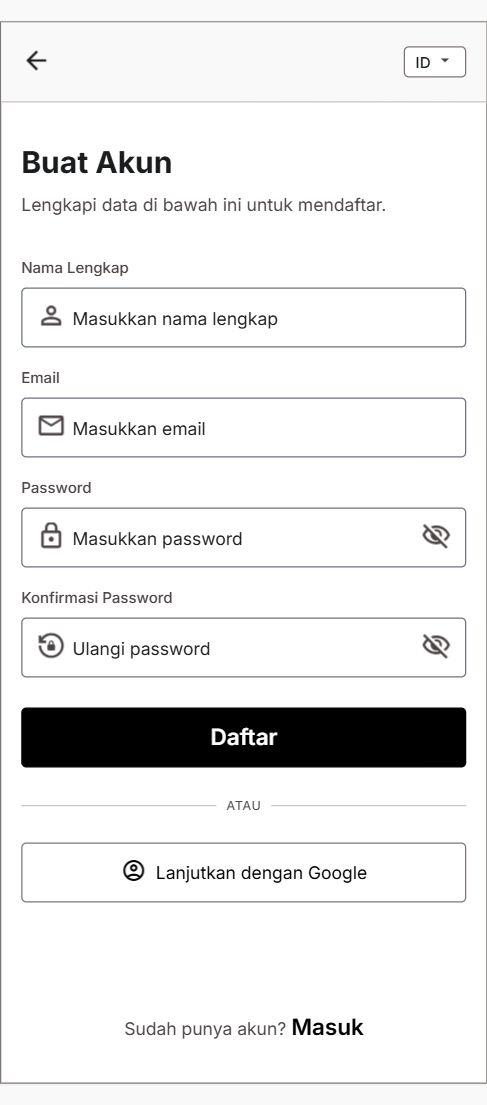
\includegraphics[width=0.35\textwidth]{wireframe_register}
        \caption{\textit{Wireframe} Halaman Registrasi Toko Baru}
        \label{fig:wf_register}
    \end{figure}

    \newpage

    \item \textbf{Halaman \textit{Login}}

    Halaman masuk akun untuk Owner maupun Kasir dengan autentikasi berbasis email dan kata sandi melalui Supabase Auth.

    \begin{figure}[H]
        \centering
        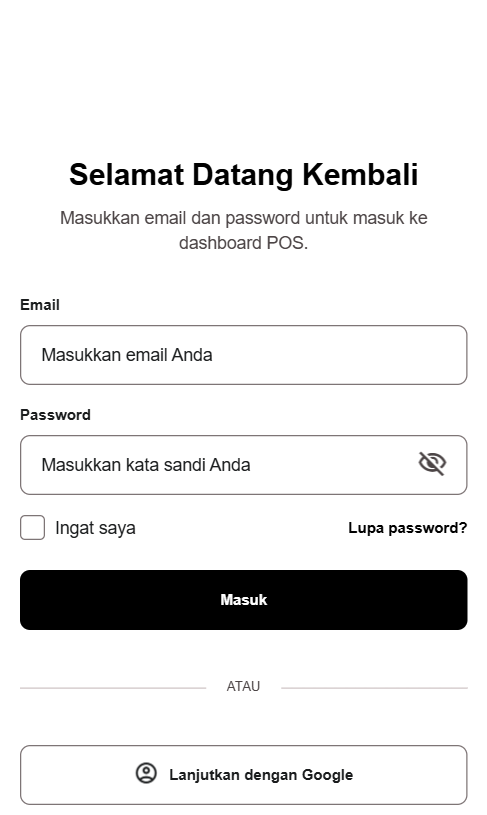
\includegraphics[width=0.45\textwidth]{wireframe_login}
        \caption{\textit{Wireframe} Halaman \textit{Login}}
        \label{fig:wf_login}
    \end{figure}

    \item \textbf{Halaman Pemilihan Toko}

    Memungkinkan pengguna yang telah \textit{login} untuk memilih toko aktif yang akan dioperasikan, terutama bagi pengguna yang terdaftar di lebih dari satu outlet.

    \begin{figure}[H]
        \centering
        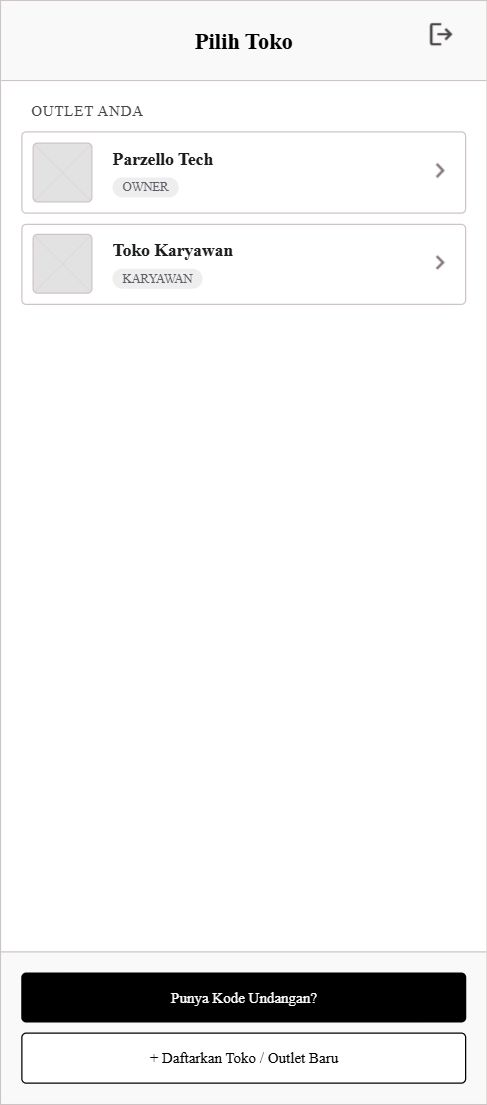
\includegraphics[width=0.45\textwidth]{wireframe_store_list}
        \caption{\textit{Wireframe} Halaman Pemilihan Toko}
        \label{fig:wf_store_list}
    \end{figure}

    \item \textbf{Halaman Dasbor Owner}

    Ringkasan performa toko yang menampilkan statistik penjualan harian, grafik tren omzet, pintasan fitur penting, dan akses cepat ke modul utama khusus Owner.

    \begin{figure}[H]
        \centering
        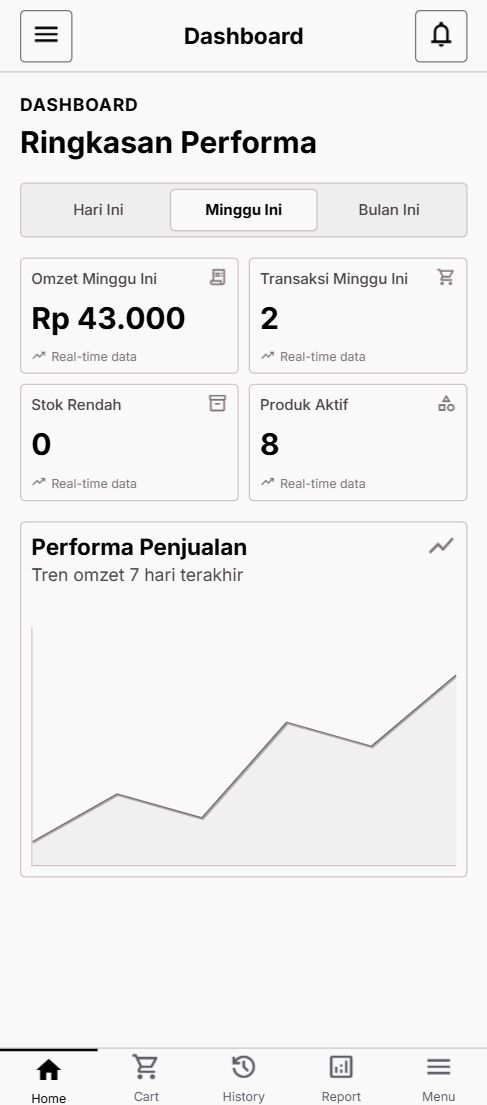
\includegraphics[width=0.45\textwidth]{wireframe_dashboard_owner}
        \caption{\textit{Wireframe} Halaman Dasbor Owner}
        \label{fig:wf_dashboard_owner}
    \end{figure}

    \item \textbf{Halaman POS (Pembayaran)}

    Layar utama kasir untuk mencari produk, menyusun keranjang pesanan, menerapkan \textit{voucher} diskon, memilih metode pembayaran, dan memproses transaksi.

    \begin{figure}[H]
        \centering
        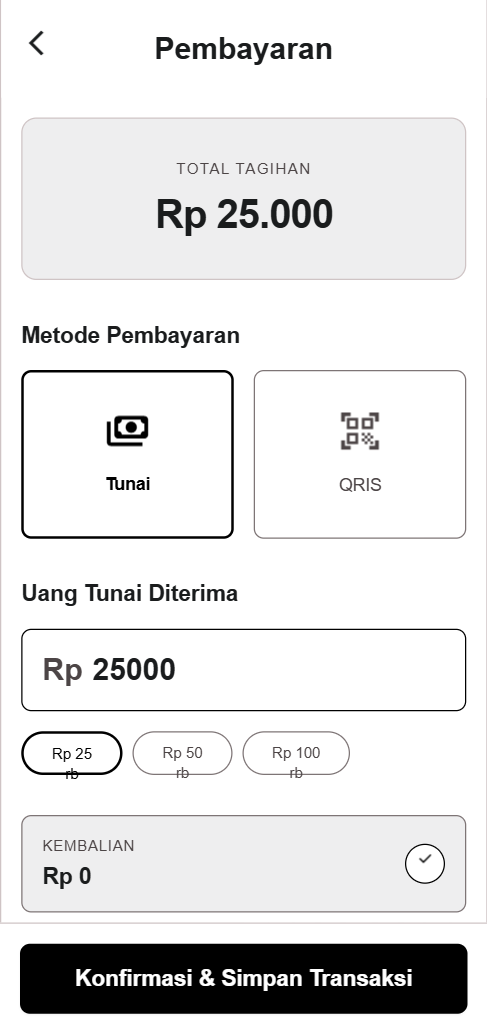
\includegraphics[width=0.45\textwidth]{wireframe_payment}
        \caption{\textit{Wireframe} Halaman POS (Pembayaran)}
        \label{fig:wf_payment}
    \end{figure}

    \item \textbf{Halaman Riwayat Transaksi}

    Menampilkan daftar transaksi yang telah dilakukan lengkap dengan fitur pencarian dan \textit{filter} berdasarkan tanggal, berguna untuk keperluan verifikasi dan audit oleh semua staf toko.

    \begin{figure}[H]
        \centering
        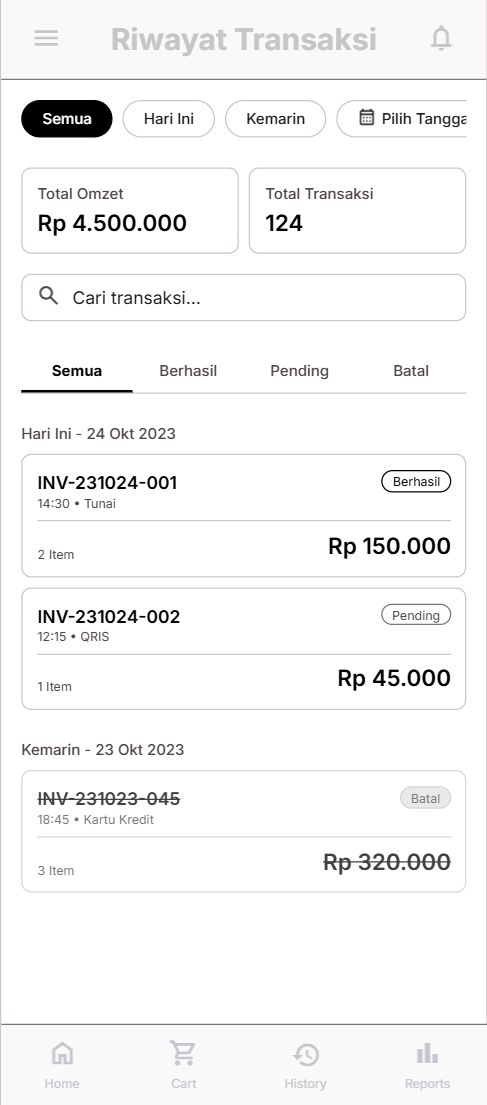
\includegraphics[width=0.45\textwidth]{wireframe_transaction_history}
        \caption{\textit{Wireframe} Halaman Riwayat Transaksi}
        \label{fig:wf_transaction_history}
    \end{figure}

    \item \textbf{Halaman Kelola Produk}

    Memungkinkan staf toko untuk menambah, menyunting, dan menghapus produk yang dijual, lengkap dengan harga, stok, SKU/\textit{barcode}, gambar produk, dan kategori.

    \begin{figure}[H]
        \centering
        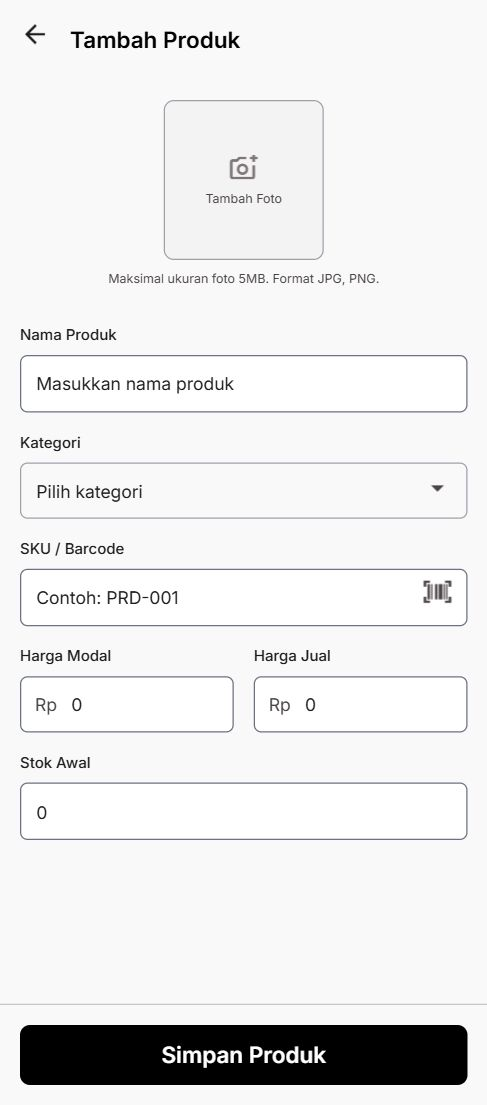
\includegraphics[width=0.45\textwidth]{wireframe_add_product}
        \caption{\textit{Wireframe} Halaman Kelola Produk}
        \label{fig:wf_add_product}
    \end{figure}

    \item \textbf{Halaman Kelola Kategori}

    Memungkinkan staf toko untuk membuat, mengedit, dan menghapus kategori produk guna mengorganisasi katalog dagangan toko dengan lebih terstruktur.

    \begin{figure}[H]
        \centering
        
\includegraphics[width=0.45\textwidth]{wireframe_manage_categories}
        \caption{\textit{Wireframe} Halaman Kelola Kategori}
        \label{fig:wf_manage_categories}
    \end{figure}

    \item \textbf{Halaman Laporan}

    Layar yang dapat diakses seluruh staf toko untuk menampilkan laporan penjualan, tren bisnis, proyeksi penjualan harian berbasis model LSTM, dan ringkasan performa operasional toko.

    \begin{figure}[H]
        \centering
        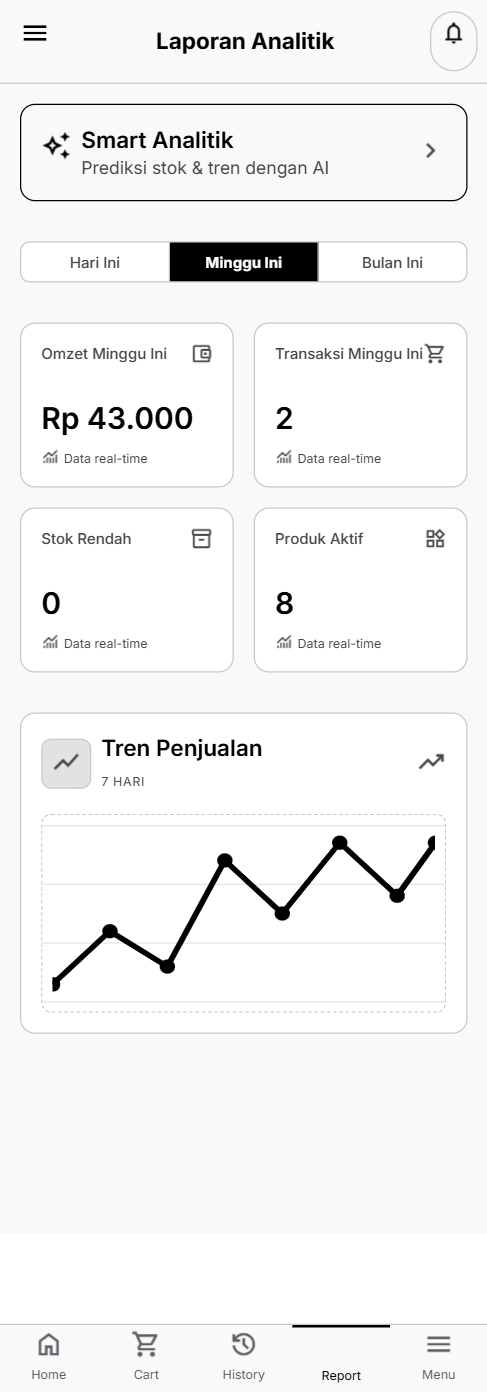
\includegraphics[width=0.45\textwidth]{wireframe_reports}
        \caption{\textit{Wireframe} Halaman Laporan}
        \label{fig:wf_reports}
    \end{figure}

    \item \textbf{Halaman Pengaturan}

    Pusat konfigurasi aplikasi dan toko yang dapat diakses oleh semua staf, dengan sejumlah menu yang hanya tersedia bagi Owner seperti pengaturan profil toko dan integrasi pembayaran.

    \begin{figure}[H]
        \centering
        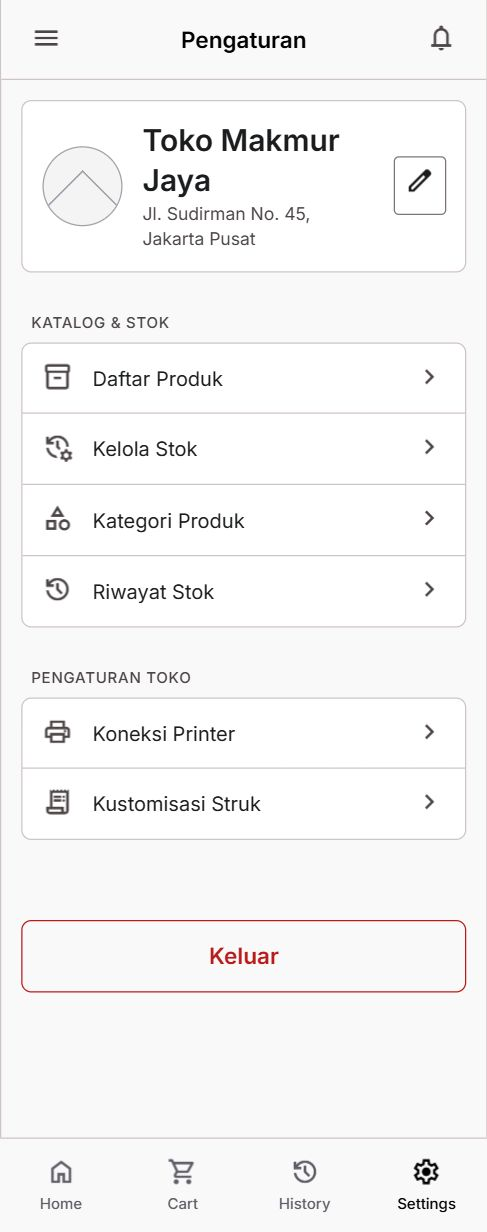
\includegraphics[width=0.45\textwidth]{wireframe_settings}
        \caption{\textit{Wireframe} Halaman Pengaturan}
        \label{fig:wf_settings}
    \end{figure}

    \item \textbf{Halaman Informasi Toko}

    Memungkinkan Owner untuk mengubah nama toko, alamat, logo outlet, dan informasi operasional lainnya yang ditampilkan kepada pelanggan.

    \begin{figure}[H]
        \centering
        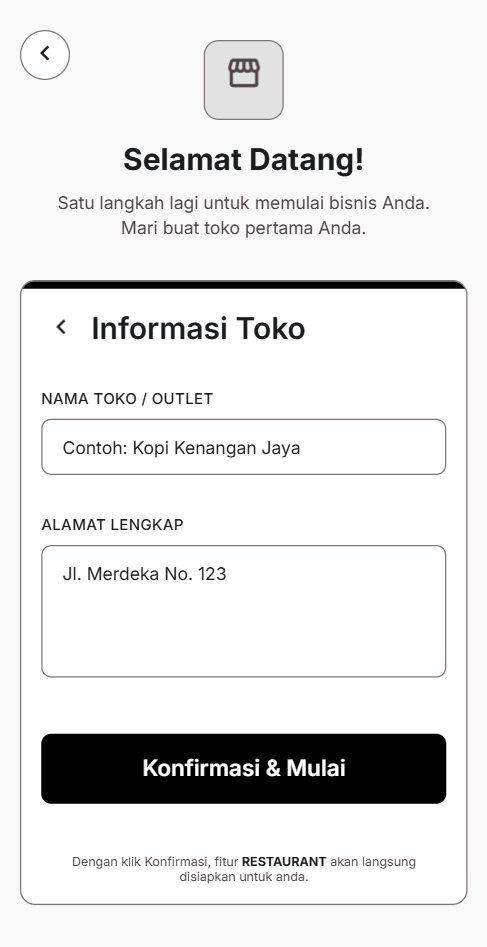
\includegraphics[width=0.45\textwidth]{wireframe_store_info}
        \caption{\textit{Wireframe} Halaman Informasi Toko}
        \label{fig:wf_store_info}
    \end{figure}

    \item \textbf{Halaman Struk Digital}

    Menampilkan pratinjau struk transaksi dalam format digital yang dapat dibagikan kepada pelanggan, mencakup rincian produk, total pembayaran, dan informasi toko.

    \begin{figure}[H]
        \centering
        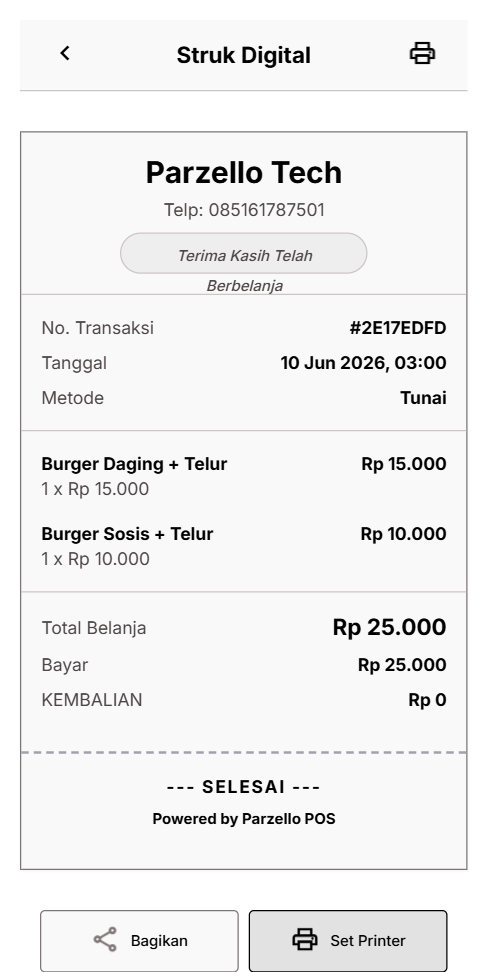
\includegraphics[width=0.45\textwidth]{wireframe_digital_receipt}
        \caption{\textit{Wireframe} Halaman Struk Digital}
        \label{fig:wf_digital_receipt}
    \end{figure}

    \item \textbf{Halaman Katalog Produk}

    Beranda mode pelanggan yang menampilkan katalog produk toko beserta kategori menu, informasi harga, dan fitur pencarian produk secara mandiri.

    \begin{figure}[H]
        \centering
        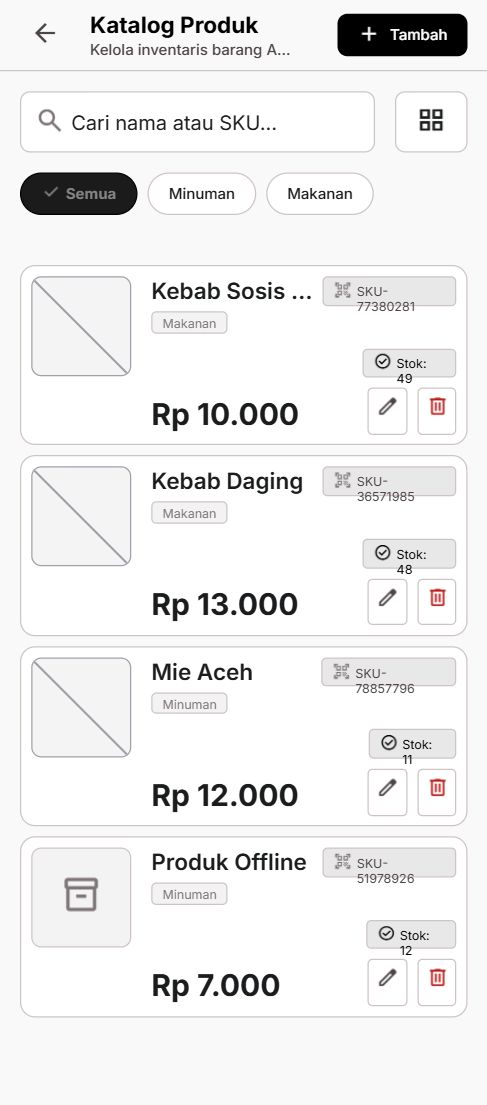
\includegraphics[width=0.45\textwidth]{wireframe_product_catalog}
        \caption{\textit{Wireframe} Halaman Katalog Produk}
        \label{fig:wf_product_catalog}
    \end{figure}

\end{enumerate}

\subsection{Teknik Pengujian}

Pengujian sistem pada penelitian ini mencakup dua pendekatan utama untuk memastikan kualitas fungsional aplikasi dan keandalan model prediksi yang diintegrasikan. Pendekatan pengujian tersebut dibagi menjadi pengujian evaluasi model prediksi penjualan dan pengujian fungsionalitas sistem secara keseluruhan menggunakan metode \textit{black box testing}.

\subsubsection{Rancangan Pengujian Evaluasi Model Prediksi}

Pengujian model prediksi dilakukan untuk mengukur kinerja dan tingkat akurasi dari algoritma \textit{Long Short-Term Memory} (LSTM) yang dikembangkan. Pengujian ini menggunakan data pengujian (\textit{testing data}) yang diambil dari data histori transaksi penjualan harian mitra UMKM. Evaluasi akurasi model diukur berdasarkan tingkat kesalahan (\textit{error}) prediksi menggunakan empat metrik utama, yaitu MAE, RMSE, sMAPE, dan MASE.

\begin{enumerate}
    \item \textbf{\textit{Mean Absolute Error} (MAE):}
    MAE digunakan untuk mengukur rata-rata selisih absolut antara nilai aktual penjualan dengan nilai hasil prediksi. Semakin kecil nilai MAE, maka model prediksi semakin akurat. Formula MAE didefinisikan sebagai berikut:
    \begin{equation}
        \text{MAE} = \frac{1}{n} \sum_{t=1}^{n} |Y_t - \hat{Y}_t|
    \end{equation}
    di mana $Y_t$ adalah nilai aktual pada hari ke-$t$, $\hat{Y}_t$ adalah nilai prediksi pada hari ke-$t$, dan $n$ adalah jumlah data pengujian.

    \item \textbf{\textit{Root Mean Square Error} (RMSE):}
    RMSE memberikan bobot lebih besar pada kesalahan prediksi yang bernilai besar karena selisihnya dikuadratkan terlebih dahulu sebelum dirata-ratakan dan ditarik akarnya. Formula RMSE didefinisikan sebagai berikut:
    \begin{equation}
        \text{RMSE} = \sqrt{\frac{1}{n} \sum_{t=1}^{n} (Y_t - \hat{Y}_t)^2}
    \end{equation}

    \item \textbf{\textit{Symmetric Mean Absolute Percentage Error} (sMAPE):}
    sMAPE digunakan untuk mengukur persentase kesalahan absolut rata-rata dengan membagi selisih absolut terhadap rata-rata dari nilai aktual dan nilai prediksi. sMAPE memberikan batas kesalahan maksimum sebesar 200\% dan bersifat lebih stabil dibandingkan MAPE konvensional ketika dihadapkan pada nilai aktual yang mendekati nol. Formula sMAPE didefinisikan sebagai berikut:
    \begin{equation}
        \text{sMAPE} = \frac{1}{n} \sum_{t=1}^{n} \frac{|Y_t - \hat{Y}_t|}{(|Y_t| + |\hat{Y}_t|) / 2} \times 100\%
    \end{equation}
    Sebagai konvensi implementasi, apabila penyebut bernilai nol (nilai aktual dan prediksi sama-sama nol), penyebut diganti dengan nilai 1 agar tidak terjadi galat pembagian dengan nol (\textit{division by zero}); konvensi inilah yang diverifikasi pada pengujian \textit{white box}.

    \item \textbf{\textit{Mean Absolute Scaled Error} (MASE):}
    MASE mengukur kesalahan absolut model prediksi relatif terhadap kesalahan absolut rata-rata dari model peramalan naif sederhana (\textit{one-step naive forecast}) secara \textit{in-sample} pada data latih. Nilai MASE kurang dari 1 menunjukkan bahwa model memiliki kinerja peramalan yang lebih baik dibandingkan metode naif. Formula MASE didefinisikan sebagai berikut:
    \begin{equation}
        \text{MASE} = \frac{\frac{1}{n} \sum_{t=1}^{n} |Y_t - \hat{Y}_t|}{\frac{1}{N-1} \sum_{i=2}^{N} |Y^{\text{train}}_i - Y^{\text{train}}_{i-1}|}
    \end{equation}
    di mana $Y^{\text{train}}_i$ adalah nilai aktual pendapatan pada data latih, dan $N$ adalah jumlah data latih aktif.
\end{enumerate}

Sebagai kriteria keberhasilan model pada diagram alur (Gambar \ref{fig:lstm_alur}), ditetapkan ambang akurasi target berupa nilai \textbf{MASE $< 1$} pada data uji, yaitu model dinyatakan layak apabila galatnya lebih kecil daripada metode naif; apabila kriteria tersebut belum terpenuhi, dilakukan iterasi penyetelan konfigurasi (\textit{hyperparameter tuning}) meliputi jumlah neuron, \textit{learning rate}, \textit{batch size}, dan bentuk target prediksi. Pengujian evaluasi ini dilakukan dengan mengukur kinerja model menggunakan pendekatan \textit{multi-seed evaluation} (10 \textit{seeds} acak) untuk memastikan stabilitas performa model LSTM terhadap variasi inisialisasi bobot awal jaringan saraf. Hasil pengujian akhir tersebut selanjutnya dibandingkan dengan model pembanding (\textit{baselines}) untuk menentukan kelayakan model LSTM. Selain itu, diuji pula skenario perbandingan performa model LSTM yang dilatih dengan dan tanpa tambahan data sintetis hasil augmentasi TimeGAN terhadap \textit{baseline} \textit{Seasonal-Naive}, guna mengukur efektivitas augmentasi data dalam memitigasi keterbatasan ukuran dataset.

\subsubsection{Rancangan Analisis Pengujian \textit{Black Box}}

Pengujian fungsional sistem pada penelitian ini menggunakan metode \textit{black box testing}, yaitu metode pengujian perangkat lunak yang berfokus pada validasi fungsional sistem dengan mengamati kesesuaian antara masukan (\textit{input}) dan keluaran (\textit{output}) yang dihasilkan, tanpa memperhatikan struktur internal kode program. Pengujian diterapkan pada fitur-fitur utama sistem untuk memastikan aplikasi berjalan sesuai dengan kebutuhan operasional pengguna.

Rancangan skenario pengujian \textit{black box} untuk fitur-fitur utama sistem POS ini dijabarkan pada Tabel \ref{tab:blackbox} berikut:

{\setstretch{1.15}
\begin{longtable}{|>{\centering\arraybackslash}p{0.6cm}|>{\raggedright\arraybackslash}p{3.0cm}|>{\raggedright\arraybackslash}p{4.7cm}|>{\raggedright\arraybackslash}p{4.7cm}|}
\caption{Skenario Pengujian \textit{Black Box}} \label{tab:blackbox} \\
\hline
\textbf{No.} & \textbf{Fitur / Fungsi} & \textbf{Skenario Pengujian} & \textbf{Hasil yang Diharapkan} \\
\hline
\endfirsthead

\multicolumn{4}{@{}l}{Tabel \thetable\ \textit{(lanjutan)}}\\
\hline
\textbf{No.} & \textbf{Fitur / Fungsi} & \textbf{Skenario Pengujian} & \textbf{Hasil yang Diharapkan} \\
\hline
\endhead

\hline
\endfoot
\hline
\endlastfoot

1 & Registrasi Toko Baru & Mengisi \textit{form} registrasi dengan email baru, kata sandi, nama toko, alamat, dan nomor HP. & Akun Owner berhasil dibuat, data toko tersimpan di \textit{database} Supabase \textit{cloud}, dan beralih ke halaman utama. \\
\hline
2 & \textit{Login} Akun & Memasukkan email dan kata sandi yang \textit{valid}/\textit{invalid} pada layar \textit{login}. & Jika \textit{valid}, pengguna masuk ke dasbor sesuai hak akses peran. Jika \textit{invalid}, sistem menampilkan pesan \textit{error} autentikasi. \\
\hline
3 & \textit{Checkout} Transaksi & Memasukkan produk ke keranjang, memilih metode bayar, dan mengonfirmasi nominal bayar. & Transaksi berhasil disimpan di \textit{database} lokal Isar DB, jumlah stok produk berkurang otomatis, dan dialihkan ke struk sukses. \\
\hline
4 & Terapkan Diskon & Memasukkan kode \textit{voucher}/nilai diskon pada keranjang belanja sebelum pembayaran. & Total belanja terpotong sesuai nilai nominal diskon/\textit{voucher} dan tercatat pada rincian nota. \\
\hline
5 & Mencetak Struk & Menghubungkan printer Bluetooth \textit{thermal} dan menekan tombol cetak struk dari riwayat transaksi. & Printer \textit{thermal} mencetak struk fisik transaksi secara lengkap (nama produk, total, tanggal, metode bayar). \\
\hline
6 & Kelola Produk & Menambah produk baru dengan nama, harga, stok, foto, dan kategori serta mengubah/menghapus produk. & Data produk baru tersimpan di \textit{database} lokal Isar DB, terdaftar pada \textit{list} produk, dan dapat diubah/dihapus. \\
\hline
7 & Kelola Kategori & Menambahkan kategori baru, menyunting nama kategori, atau menghapus kategori produk. & Kategori berhasil dibuat, muncul sebagai opsi \textit{filter} menu, dan diperbarui secara \textit{real-time}. \\
\hline
8 & Audit Mutasi Stok & Melakukan transaksi/penyesuaian stok, lalu membuka halaman riwayat mutasi stok. & Riwayat keluar-masuk barang tercatat pada \textit{log} \textit{stock\_history} dengan jenis mutasi yang sesuai. \\
\hline
9 & Dasbor Ringkasan & Membuka dasbor laporan penjualan harian, mingguan, dan grafik visualisasi omzet. & Menampilkan statistik ringkasan omzet, total transaksi harian, dan grafik visualisasi garis yang akurat. \\
\hline
10 & \textit{Smart Analytics} & Membuka layar \textit{Smart Analytics} dengan koneksi internet aktif. & Grafik prediksi penjualan 7 hari ke depan dari layanan API prediksi berhasil ditampilkan dan tersimpan sebagai \textit{snapshot}. \\
\hline
11 & \textit{Broadcast} Notifikasi & Owner mengirim pesan \textit{broadcast} kepada staf toko melalui menu notifikasi. & Notifikasi \textit{broadcast} diterima dan muncul di perangkat kasir secara \textit{real-time}. \\
\hline
12 & Sinkronisasi \textit{Offline} & Mematikan koneksi internet (luring), membuat transaksi lokal, lalu mengaktifkan internet kembali (daring). & Transaksi disimpan secara lokal di Isar DB (\textit{offline-first}), lalu terunggah otomatis ke Supabase \textit{cloud} saat internet aktif kembali. \\
\hline
13 & Kelola Staf Karyawan & Owner menambahkan akun staf kasir baru dan mengubah peran staf. & Akun staf berhasil terdaftar pada toko dengan peran yang sesuai; menu ini tidak dapat diakses oleh Kasir. \\
\hline
14 & Atur Profil Toko & Owner mengubah nama, alamat, dan logo toko pada menu pengaturan. & Informasi profil toko berhasil diperbarui dan tampil pada struk serta katalog; menu ini eksklusif untuk Owner. \\
\hline
\end{longtable}
}

\subsubsection{Rancangan Analisis Pengujian \textit{White Box}}

Selain pengujian fungsional \textit{black box}, penelitian ini turut menerapkan pengujian \textit{white box} secara terbatas (\textit{lightweight}) yang berfokus pada verifikasi kebenaran logika internal dan jalur eksekusi kode (\textit{code path}) pada fungsi-fungsi kritis di layanan API prediksi, tanpa memandang antarmuka luarnya. Pengujian ini dilakukan dengan menelusuri (\textit{trace}) jalur logika kode secara manual menggunakan data masukan yang telah diketahui nilai keluarannya, kemudian membandingkan hasil eksekusi aktual terhadap hasil kalkulasi manual sebagai acuan kebenaran (\textit{ground truth}). Tiga fungsi inti yang menjadi target pengujian \textit{white box} adalah:
\begin{enumerate}
    \item Fungsi perhitungan \textit{Seasonal-Naive} (\texttt{by\_dow}), untuk memverifikasi jalur percabangan logika ketika jumlah data historis per hari kerja mencukupi ($\geq k$), tidak mencukupi ($<k$), maupun tidak tersedia sama sekali (\textit{fallback}).
    \item Fungsi metrik evaluasi sMAPE dan MASE, untuk memverifikasi jalur penanganan kasus pembagian dengan nilai penyebut nol atau mendekati nol agar tidak menghasilkan galat pembagian (\textit{division by zero}).
    \item Fungsi peramalan rekursif (\texttt{forecast\_hybrid\_stable}), untuk memverifikasi jalur eksekusi tiga mekanisme pengaman secara berurutan, yaitu \textit{clipping} \textit{log-return}, \textit{damping factor}, dan \textit{safety rail} nominal omzet.
\end{enumerate}

\subsection{Indikator Keberhasilan Penelitian}

Keberhasilan penelitian ini diukur melalui indikator-indikator berikut, yang pencapaiannya dijawab pada Bab IV dan Bab V:
\begin{enumerate}
    \item Aplikasi \textit{Point of Sale} (POS) \textit{mobile} berfungsi membantu pelaku UMKM dalam mengelola transaksi penjualan, inventaris produk, dan laporan keuangan secara efisien dengan kemampuan operasional \textit{offline-first}, yang divalidasi melalui pengujian fungsional \textit{Black Box}.
    \item Metode LSTM terimplementasi pada sistem dan kinerjanya terukur secara objektif menggunakan metrik evaluasi kesalahan prediksi terhadap model pembanding (\textit{baseline}).
    \item Sistem mampu menyajikan informasi prediksi dan laporan penjualan dalam bentuk visualisasi grafik yang mudah dipahami oleh pengguna, khususnya pelaku UMKM.
\end{enumerate}

%%=============================================================
%% BAB IV - HASIL DAN PEMBAHASAN
%%=============================================================
\chapter[HASIL DAN PEMBAHASAN]{\\ HASIL DAN PEMBAHASAN}

Bab ini menyajikan hasil rancang bangun dan pembahasan sistem Point of Sale (POS) dengan fitur prediksi penjualan harian menggunakan metode Long Short-Term Memory (LSTM). Pembahasan dibagi menjadi tujuh bagian utama, yaitu hasil implementasi sistem, \textit{preprocessing} data, implementasi dan pelatihan model peramalan, evaluasi model, hasil pengujian sistem, pembahasan hasil penelitian, serta keterbatasan sistem dan penelitian.

\section{Hasil Implementasi Sistem}

Bagian ini memaparkan realisasi fisik dari rancangan sistem yang telah disusun pada Bab III, yang mencakup implementasi antarmuka aplikasi mobile (kasir dan owner), implementasi backend dan basis data cloud (Supabase), serta implementasi layanan prediksi (API) di sisi server.

\subsection{Implementasi Antarmuka (UI)}

Aplikasi mobile dikembangkan menggunakan framework Flutter dengan bahasa pemrograman Dart. Komponen antarmuka pengguna disesuaikan dengan rancangan wireframe untuk menjamin kenyamanan operasional kasir. Berikut adalah penjelasan mengenai implementasi antarmuka layar utama aplikasi:

\begin{enumerate}
    \item \textbf{Halaman Registrasi Toko Baru}:
    Halaman ini merupakan langkah awal inisialisasi sistem yang digunakan oleh Owner untuk mendaftarkan akun baru dan meregistrasikan profil outlet toko. Form registrasi memuat kolom input nama lengkap, email, kata sandi, nama toko, alamat outlet, dan nomor telepon.
    
    \item \textbf{Halaman Login}:
    Menyediakan fasilitas autentikasi pengguna menggunakan email dan kata sandi. Keamanan akses diatur melalui layanan autentikasi Supabase. Sistem secara otomatis mengidentifikasi peran akun (Owner atau Kasir) setelah login berhasil untuk menentukan batasan hak akses menu.
    
    \item \textbf{Halaman Pemilihan Toko}:
    Layar ini ditujukan bagi pengguna yang terdaftar di lebih dari satu outlet toko merchant. Pengguna dapat memilih outlet aktif yang ingin dioperasikan sebelum diarahkan ke halaman dasbor utama.
    
    \item \textbf{Halaman Dasbor Owner}:
    Menampilkan visualisasi ringkasan kinerja penjualan toko saat ini, seperti grafik tren omzet penjualan harian, jumlah total transaksi, total nominal omzet harian, dan ringkasan stok produk yang menipis sebagai peringatan restock cepat.
    
    \item \textbf{Halaman POS (Pembayaran / Checkout)}:
    Merupakan layar operasional utama kasir untuk memproses transaksi. Kasir dapat memilih produk, memasukkan jumlah barang ke keranjang belanja, menerapkan diskon atau voucher, memilih metode pembayaran (Tunai, QRIS, atau Transfer), serta menyelesaikan transaksi pembayaran.
    
    \item \textbf{Halaman Riwayat Transaksi}:
    Menampilkan daftar nota transaksi penjualan yang telah diselesaikan. Halaman ini memuat informasi detail nomor invoice, tanggal transaksi, nama kasir, total nominal pembayaran, dan status sinkronisasi cloud.
    
    \item \textbf{Halaman Kelola Produk dan Kategori}:
    Menyediakan antarmuka bagi staf toko untuk mengelola inventaris produk (menambah, mengubah, dan menghapus produk) beserta pengelompokan berdasarkan kategori produk. Form produk memuat nama produk, harga jual, stok fisik, barcode/SKU, dan gambar produk.
    
    \item \textbf{Halaman Laporan (Analitik AI \& Prediksi LSTM)}:
    Menampilkan visualisasi grafik data penjualan aktual historis berdampingan dengan kurva proyeksi penjualan harian untuk 7 hari ke depan yang diperoleh dari layanan API prediksi penjualan.
    
    \item \textbf{Halaman Pengaturan dan Profil Toko}:
    Memungkinkan staf toko untuk mengubah konfigurasi dasar aplikasi, dengan menu pengaturan profil outlet toko (logo, nama, alamat) dan pengelolaan akun karyawan/staf kasir yang khusus tersedia bagi Owner.
    
    \item \textbf{Halaman Struk Digital dan Katalog Mandiri}:
    Halaman struk digital menampilkan pratinjau struk fisik transaksi yang dapat dibagikan langsung ke pelanggan via aplikasi pesan instan. Layar katalog mandiri menyediakan daftar menu produk yang dapat dipindai oleh pelanggan untuk melihat daftar harga barang secara langsung.
\end{enumerate}

\subsection{Implementasi Backend dan Basis Data Cloud}

Infrastruktur backend cloud diimplementasikan menggunakan platform Supabase BaaS dengan database PostgreSQL. Struktur relasional database diwujudkan melalui sembilan tabel utama yang saling terhubung:
\begin{enumerate}
    \item \textit{stores}: Menyimpan data identitas outlet merchant (id, nama, alamat, nomor HP, URL logo, created\_at).
    \item \textit{store\_members}: Mengatur relasi hak akses pengguna dengan peran Owner atau Karyawan di masing-masing outlet.
    \item \textit{categories}: Mengelola daftar kategori pengelompokan produk.
    \item \textit{products}: Menyimpan katalog inventaris barang (id, nama, harga, stok, barcode, URL foto, is\_synced, is\_deleted).
    \item \textit{transactions}: Menyimpan data nota induk transaksi penjualan (id, total belanja, metode pembayaran, kasir\_id, created\_at).
    \item \textit{transaction\_items}: Menyimpan rincian item produk yang terjual pada setiap transaksi penjualan (id, transaksi\_id, produk\_id, jumlah, harga).
    \item \textit{stock\_history}: Mencatat log audit mutasi perubahan stok produk (stok masuk, keluar, penjualan, audit manual).
    \item \textit{notifications}: Mengelola pesan notifikasi sistem dan info siaran antar staf toko secara real-time.
    \item \textit{smart\_analytics\_snapshots}: Menyimpan riwayat \textit{snapshot} hasil analitik prediksi LSTM setiap kali fitur \textit{Smart Analytics} dijalankan, sehingga hasil analisis sebelumnya dapat ditinjau kembali tanpa memanggil ulang model.
\end{enumerate}

Keamanan akses data antar-outlet dijamin melalui penerapan kebijakan Row Level Security (RLS) di database PostgreSQL. Kebijakan ini memastikan bahwa pengguna (kasir/owner) hanya dapat membaca dan menulis data yang memiliki \textit{store\_id} yang sesuai dengan toko tempat mereka terdaftar.

\subsection{Implementasi Layanan Prediksi (API)}

Modul kecerdasan buatan untuk kalkulasi prediksi penjualan harian dikembangkan menggunakan Python dan terdiri atas dua bagian yang saling melengkapi. Bagian pertama adalah \textit{pipeline} riset berbasis Jupyter Notebook yang melatih model peramalan LSTM (TensorFlow/Keras) pada tiga granularitas waktu (harian, mingguan, dan bulanan) beserta eksperimen augmentasi data sintetis TimeGAN (PyTorch). Bagian kedua adalah layanan API produksi berbasis \textit{framework} Flask yang di-\textit{deploy} pada platform Hugging Face dan diintegrasikan langsung dengan aplikasi POS, sehingga beban komputasi peramalan terpisah dari beban kerja transaksional kasir.

Layanan API produksi menyediakan tujuh \textit{endpoint} REST dengan fungsi sebagai berikut:
\begin{enumerate}
    \item \textbf{Endpoint Prediksi Penjualan} (\texttt{/api/predict/daily}, \texttt{/api/predict/weekly}, \texttt{/api/predict/monthly}): Meramalkan omzet ke depan dengan tanggal prediksi yang otomatis melewati hari tutup (akhir pekan serta libur semester Januari/Juli). Berdasarkan hasil evaluasi komparatif pada penelitian ini (Subbab 4.4), metode penyaji yang dipilih pada \textit{endpoint} produksi adalah metode statistik paling stabil, yaitu \textit{Seasonal-Naive} ($k=4$, rata-rata empat kemunculan terakhir hari yang sama — kompromi antara responsivitas terhadap tren terbaru dan peredaman fluktuasi acak, setara dengan rentang sekitar satu bulan hari sejenis) untuk harian, \textit{Mean-4} untuk mingguan, dan \textit{Mean-3} untuk bulanan, dengan prediksi \textit{Naive} disertakan sebagai pembanding; sedangkan model LSTM hasil pelatihan didokumentasikan sebagai artefak riset (\texttt{.keras}).
    \item \textbf{Endpoint Rekomendasi Operasional} (\texttt{/api/recommendations/stock} dan \texttt{/api/recommendations/target}): Menghasilkan rekomendasi alokasi anggaran belanja per kategori produk dan kuantitas stok produk teratas berdasarkan proyeksi omzet (dilengkapi \textit{safety buffer} 15\% dan peringatan khusus produk mudah basi), serta tiga tingkatan target omzet harian (konservatif, moderat, dan agresif) berbasis statistik 15 hari aktif terakhir.
    \item \textbf{Endpoint Pencatatan dan Status} (\texttt{/api/sales/record} dan \texttt{/api/status}): Menerima rekap penjualan harian dari aplikasi POS dan memperbaruinya ke dataset historis (\textit{upsert} per tanggal) agar dasar peramalan selalu mengikuti data terkini, serta memeriksa kesehatan layanan dan ketersediaan berkas data.
\end{enumerate}

Aplikasi Flutter memanggil \textit{endpoint} tersebut secara langsung melalui HTTPS dengan \textit{payload} agregat penjualan tanpa informasi identitas pelanggan, kemudian menyimpan hasil analisis sebagai \textit{snapshot} pada tabel \textit{smart\_analytics\_snapshots} di Supabase.

Inti implementasi \textit{endpoint} prediksi harian pada berkas \texttt{app.py} disajikan pada Kode Program~\ref{lst:flask_daily} (dipersingkat). Metode \textit{Seasonal-Naive} dihitung dengan merata-ratakan $k$ kemunculan terakhir dari setiap hari kerja yang sama, dan tanggal prediksi dihasilkan dengan melewati hari tutup.

\begin{lstlisting}[caption={Implementasi Endpoint Prediksi Harian Seasonal-Naive (\texttt{app.py})}, label={lst:flask_daily}]
@app.route('/api/predict/daily', methods=['GET', 'POST'])
def predict_daily():
    data = request.get_json(silent=True) or {}
    n_days = int(data.get("n_days", 7))
    k = int(data.get("k", 4))
    dfa = get_daily_dataframe(data.get("history", None))
    last_date = dfa['date'].max()

    # Seasonal-Naive: rata-rata k kemunculan terakhir
    # dari hari kerja yang sama (0=Senin ... 4=Jumat)
    by_dow = {}
    for dow in range(5):
        dow_data = dfa[dfa['day_of_week'] == dow]['revenue']
        if len(dow_data) >= k:
            by_dow[dow] = dow_data.tail(k).mean()
        elif len(dow_data) > 0:
            by_dow[dow] = dow_data.mean()
        else:
            by_dow[dow] = dfa['revenue'].tail(10).mean()

    # Naive: prediksi = omzet hari kerja terakhir
    naive_value = float(dfa['revenue'].iloc[-1])

    # Tanggal prediksi otomatis melewati hari tutup
    future_dates = generate_future_business_days(last_date, n_days)
    predictions = []
    for dt in future_dates:
        pred_sn = int(round(by_dow.get(dt.weekday(), naive_value)))
        predictions.append({
            "date": dt.strftime('%Y-%m-%d'),
            "predicted_revenue_seasonal_naive": pred_sn,
            "predicted_revenue_naive": int(round(naive_value))})
    return jsonify({"predictions": predictions}), 200
\end{lstlisting}

\section{Preprocessing Data}

Bagian ini menjelaskan tahapan pengolahan data sebelum digunakan untuk melatih model peramalan, mencakup deskripsi dan eksplorasi awal dataset, serta pra-pemrosesan dan pembentukan sequence data latih.

\subsection{Deskripsi Data dan Eksplorasi Awal}

Data yang digunakan dalam pengujian model peramalan ini merupakan rekapitulasi transaksi penjualan harian kantin EatsTEDI UGM pada periode 26 Agustus 2024 hingga 20 Juni 2026. Setelah dilakukan agregasi nilai transaksi per hari dan penyaringan terhadap hari-hari non-aktif (di mana kantin tutup), diperoleh total sebanyak 313 hari aktif bisnis. Statistik ringkas mengenai dataset pendapatan harian ini disajikan pada Tabel \ref{tab:statistik_revenue_harian}.

\begin{table}[H]
\setstretch{1.2}
\centering
\caption{Statistik Ringkas Dataset Pendapatan Harian}
\label{tab:statistik_revenue_harian}
\begin{tabular}{|l|l|}
\hline
\textbf{Karakteristik} & \textbf{Nilai} \\ \hline
Jumlah hari aktif & 313 hari \\ \hline
Rentang waktu & 26 Agu 2024 -- 20 Jun 2026 \\ \hline
Total revenue (omzet) & Rp 471.200.494,00 \\ \hline
Rata-rata revenue per hari aktif & Rp 1.505.433,00 \\ \hline
Revenue tertinggi & Rp 3.738.500,00 (6 Mei 2026) \\ \hline
\end{tabular}
\end{table}

Hasil eksplorasi awal menunjukkan bahwa deret data pendapatan harian kantin EatsTEDI bersifat sangat fluktuatif dan dipengaruhi secara kuat oleh kalender akademis universitas. Terdapat pola penurunan tajam hingga bernilai Rp 0 pada masa libur semester mahasiswa (sepanjang bulan Januari dan Juli) serta pola musiman mingguan di mana penjualan menurun secara bertahap menjelang akhir pekan. Pola musiman tahunan tidak dapat teramati secara penuh karena rentang waktu data yang tersedia kurang dari dua tahun, sehingga deret waktu ini tergolong pendek (\textit{short time-series}) untuk standar pemodelan berbasis \textit{deep learning} yang membutuhkan volume data historis yang besar.

\subsection{Pra-pemrosesan dan Pembentukan Sequence}

Pemodelan peramalan pada penelitian ini difokuskan pada granularitas harian dengan strategi prediksi satu langkah ke depan (\textit{one-step-ahead prediction}). Untuk mengatasi variansi data yang ekstrem akibat fluktuasi harian yang sangat tajam, target peramalan tidak diprediksi menggunakan bentuk nilai nominal mentah, melainkan menggunakan bentuk \textit{log-return} (selisih logaritmik) pendapatan antar hari aktif yang berurutan. Pendekatan residual ini dirancang agar model cukup mempelajari koreksi atau deviasi nilai pendapatan dari hari aktif sebelumnya, sehingga model secara tidak langsung mewarisi sifat autokorelasi jangka pendek yang kuat pada deret waktu transaksi.

Variabel masukan (\textit{features}) terdiri atas nilai log-return pendapatan target dan enam fitur kalender yang dikodekan secara siklik (\textit{cyclical encoding} sinus-kosinus untuk nomor minggu dalam setahun, bulan, dan hari kerja aktif) serta variabel biner Ramadan. Variabel jumlah transaksi harian dan kuantitas produk terjual secara sengaja dikeluarkan dari variabel masukan model prediksi untuk menghindari kebocoran data (\textit{data leakage}), karena kedua nilai tersebut belum tersedia saat modul peramalan dijalankan untuk memprediksi hari berikutnya. Proses penskalaan data dilakukan menggunakan metode \textit{Min-Max Scaling} yang dipasang (\textit{fit}) hanya pada data latih untuk mencegah terjadinya kebocoran informasi dari data uji.

Pembagian dataset dilakukan secara kronologis (\textit{chronological split}) dengan rasio 70\% untuk data latih (\textit{train set}), 15\% untuk data validasi (\textit{validation set}), dan 15\% untuk data uji (\textit{test set}). Pembentukan urutan temporal (\textit{sequence}) dilakukan menggunakan panjang \textit{look-back} sebesar 7 hari aktif terakhir. Rincian pembagian data serta dimensi sequence disajikan pada Tabel \ref{tab:pembagian_data_sequence}.

\begin{table}[H]
\setstretch{1.2}
\centering
\caption{Pembagian Dataset dan Dimensi Sequence}
\label{tab:pembagian_data_sequence}
\begin{tabular}{|l|c|c|c|}
\hline
\textbf{Subset Data} & \textbf{Jumlah Hari} & \textbf{Jumlah Sequence} & \textbf{Dimensi Masukan} \\ \hline
Latih (\textit{train}) & 219 & 212 & (212, 7, 8) \\ \hline
Validasi (\textit{val}) & 46 & 39 & (39, 7, 8) \\ \hline
Uji (\textit{test}) & 48 & 41 & (41, 7, 8) \\ \hline
\end{tabular}
\end{table}

Implementasi pra-pemrosesan data — meliputi penyaringan hari aktif, transformasi target \textit{log-return}, dan pengodean siklik fitur kalender — disajikan pada Kode Program~\ref{lst:preprocessing}.

\begin{lstlisting}[caption={Pra-pemrosesan Data: Filter Hari Aktif, Log-Return, dan Fitur Siklik}, label={lst:preprocessing}]
df = pd.read_csv(DAILY_CSV, parse_dates=['date'])
# Hanya hari aktif (revenue > 0) yang dilatih ke model
dfa = df[df['revenue'] > 0].copy() \
        .sort_values('date').reset_index(drop=True)

dfa['rev_log'] = np.log1p(dfa['revenue'])
# TARGET: log-return (perubahan pendapatan harian)
dfa['logret']  = dfa['rev_log'].diff().fillna(0.0)
# Pengodean siklik sinus-kosinus fitur kalender
dfa['week_sin']  = np.sin(2*np.pi*dfa['week_of_year']/52)
dfa['week_cos']  = np.cos(2*np.pi*dfa['week_of_year']/52)
dfa['month_sin'] = np.sin(2*np.pi*dfa['month']/12)
dfa['month_cos'] = np.cos(2*np.pi*dfa['month']/12)
dfa['dow_sin']   = np.sin(2*np.pi*dfa['day_of_week']/5)
dfa['dow_cos']   = np.cos(2*np.pi*dfa['day_of_week']/5)

# 'logret' wajib kolom pertama (kolom target)
FEATURES = ['logret','week_sin','week_cos','month_sin',
            'month_cos','dow_sin','dow_cos','is_ramadan']

# Pembagian kronologis 70/15/15 (tanpa pengacakan)
n = len(dfa); n_tr = int(n*0.70); n_va = int(n*0.15)
df_tr = dfa.iloc[:n_tr]
df_va = dfa.iloc[n_tr:n_tr+n_va]
df_te = dfa.iloc[n_tr+n_va:]
\end{lstlisting}

\section{Implementasi dan Pelatihan Model Peramalan}

Bagian ini memaparkan implementasi arsitektur model LSTM beserta skenario eksperimen, hasil pelatihan model, implementasi augmentasi data sintetis TimeGAN, dan implementasi mekanisme peramalan rekursif untuk kebutuhan visualisasi jangka pendek pada aplikasi.

\subsection{Arsitektur Model dan Skenario Eksperimen}

Arsitektur model peramalan yang diimplementasikan adalah LSTM satu lapis (\textit{single-layer LSTM}) dengan 24 \textit{hidden units}, diikuti oleh lapisan \textit{Dropout} dengan laju 0,1 untuk regularisasi, satu lapisan \textit{Dense} dengan 16 neuron beraktivasi \textit{Rectified Linear Unit} (ReLU), dan diakhiri oleh satu lapisan keluaran (\textit{output layer}) tunggal beraktivasi linear. Model ini dirancang secara minimalis dengan total parameter terlatih hanya sebanyak 3.585 parameter. Pemilihan model berkapasitas rendah ini didasarkan pada jumlah data latih yang sangat terbatas (212 sampel sequence), sehingga penggunaan model LSTM berkapasitas besar (\textit{stacked layers}) akan berisiko tinggi memicu kegagalan konvergensi pelatihan atau bias \textit{overfitting}. Proses optimasi menggunakan metode Adam dengan \textit{learning rate} awal sebesar $5 \times 10^{-4}$, fungsi kerugian (\textit{loss function}) MSE, serta didukung \textit{callbacks} \textit{EarlyStopping} dan \textit{ReduceLROnPlateau}. Konstruksi arsitektur model beserta konfigurasi pelatihannya disajikan pada Kode Program~\ref{lst:build_lstm}.

\begin{lstlisting}[caption={Konstruksi Arsitektur LSTM Tersederhanakan dan Konfigurasi Pelatihan}, label={lst:build_lstm}]
LOOK_BACK = 7   # jendela masukan: 7 hari aktif
HORIZON   = 1   # prediksi 1 langkah ke depan
UNITS     = 24
DROPOUT   = 0.1

def build_lstm():
    m = Sequential([
        LSTM(UNITS, input_shape=(LOOK_BACK, len(FEATURES))),
        Dropout(DROPOUT),
        Dense(16, activation='relu'),
        Dense(HORIZON)
    ], name='lstm_hybrid_residual')
    m.compile(optimizer=Adam(5e-4), loss='mse', metrics=['mae'])
    return m

cb = [EarlyStopping('val_loss', patience=20,
                    restore_best_weights=True),
      ReduceLROnPlateau('val_loss', factor=0.5,
                        patience=8, min_lr=1e-6)]

model = build_lstm()
hist  = model.fit(X_tr, y_tr, validation_data=(X_va, y_va),
                  epochs=200, batch_size=16, callbacks=cb)
\end{lstlisting}

\subsection{Hasil Pelatihan Model}

Pada konfigurasi akhir model tersederhanakan, proses pelatihan berjalan secara stabil di mana galat validasi menunjukkan tren penurunan yang konsisten melampaui \textit{epoch} pertama. Mekanisme \textit{EarlyStopping} berhasil menghentikan proses pelatihan dan mengembalikan bobot terbaik model sebelum terjadi gejala \textit{overfitting}. Hal ini berbanding terbalik dengan uji coba pada konfigurasi awal penelitian yang menggunakan arsitektur jaringan saraf berskala besar dan target berupa nilai nominal mentah, di mana model mengalami kolaps (\textit{model collapse}) dengan galat validasi terbaik yang dicapai langsung pada \textit{epoch} pertama (model tidak melakukan pembelajaran) dan menghasilkan prediksi bernilai rendah yang konstan secara sistematis. Penyederhanaan arsitektur, pemilihan target \textit{log-return}, serta pembatasan horizon menjadi satu langkah ke depan terbukti mampu memperbaiki performa pelatihan secara signifikan, di mana nilai MAE uji terbaik model LSTM mengalami penurunan drastis dari sekitar Rp 1.805.196,00 pada konfigurasi awal menjadi berkisar antara Rp 500.000,00 hingga Rp 600.000,00 pada konfigurasi akhir. Iterasi dari konfigurasi awal (arsitektur besar, target nominal) menuju konfigurasi akhir tersederhanakan inilah yang merupakan realisasi dari \textit{loop} \textit{hyperparameter tuning} dengan kriteria akurasi (MASE $< 1$) pada diagram alur Gambar \ref{fig:lstm_alur}; meskipun kriteria MASE $< 1$ pada akhirnya tidak tercapai oleh konfigurasi manapun, iterasi dihentikan pada konfigurasi terbaik dan keputusan produksi dialihkan ke metode \textit{baseline} sebagaimana dibahas pada Subbab 4.4. Grafik kurva kerugian pelatihan model ditunjukkan pada Gambar \ref{fig:lstm_kurva_training}.

\begin{figure}[H]
    \centering
    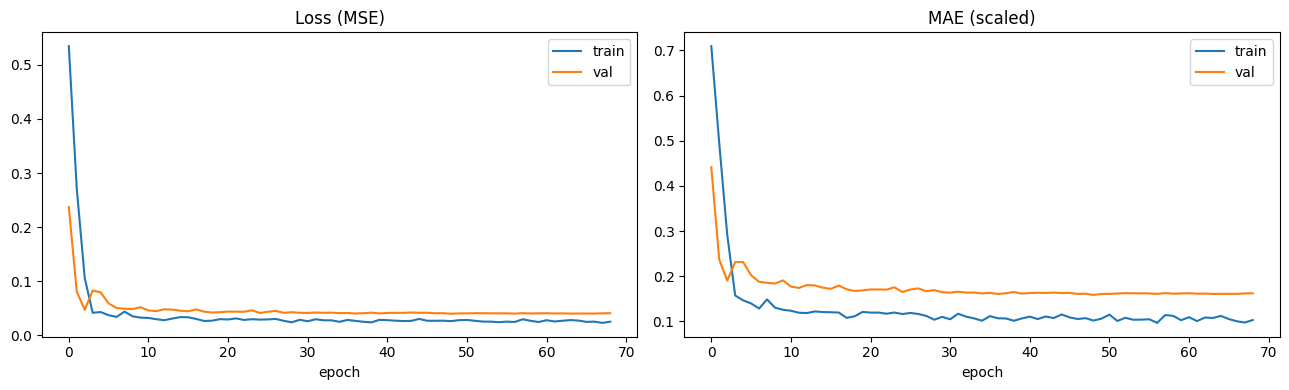
\includegraphics[width=0.7\textwidth]{Gambar/lstm_harian_disederhanakan_plot_kurva_training}
    \caption{Kurva Kerugian Pelatihan (\textit{Training Loss Curve}) Model LSTM}
    \label{fig:lstm_kurva_training}
\end{figure}

\subsection{Implementasi Augmentasi Data Sintetis TimeGAN}

Sebagai upaya mitigasi terhadap keterbatasan ukuran dataset yang menjadi akar penyebab ketidakstabilan model LSTM, dilakukan eksperimen augmentasi data sintetis menggunakan \textbf{TimeGAN} (Yoon et al., 2019). Model TimeGAN yang diimplementasikan dengan PyTorch dilatih pada jendela deret waktu sepanjang 24 hari aktif dengan tiga fitur numerik (omzet, jumlah transaksi, dan kuantitas terjual) melalui tiga fase pelatihan (\textit{autoencoder}, \textit{supervised}, dan \textit{joint adversarial training}) masing-masing sebanyak 600 \textit{epoch}, kemudian menghasilkan 200 sekuens data harian sintetis. Pada skenario ini, model LSTM multi-langkah (\textit{look-back} 14 hari aktif, horizon 7 hari) selanjutnya dilatih dalam dua kondisi: hanya menggunakan 219 sekuens data riil (\textit{baseline real-only}), dan menggunakan gabungan data riil dengan 298 sekuens sintetis (rasio augmentasi 1,5). Hasil evaluasi perbandingan kedua kondisi tersebut disajikan pada Subbab 4.4.3.

Cuplikan implementasi dua dari lima jaringan penyusun TimeGAN pada berkas \texttt{TimeGAN.py} — jaringan \textit{embedder} yang memetakan data riil ke ruang laten dan \textit{generator} yang memetakan derau acak menjadi representasi laten sintetis — disajikan pada Kode Program~\ref{lst:timegan}.

\begin{lstlisting}[caption={Implementasi Jaringan \textit{Embedder} dan \textit{Generator} TimeGAN (PyTorch)}, label={lst:timegan}]
class EmbedderNet(nn.Module):
    """Memetakan data nyata X -> representasi laten H."""
    def __init__(self):
        super().__init__()
        self.rnn  = nn.GRU(NUM_FEAT, HIDDEN_DIM,
                           NUM_LAYERS, batch_first=True)
        self.proj = nn.Sequential(
            nn.Linear(HIDDEN_DIM, HIDDEN_DIM), nn.Sigmoid())

    def forward(self, x):
        h, _ = self.rnn(x)
        return self.proj(h)

class GeneratorNet(nn.Module):
    """Memetakan noise Z -> laten sintetis E."""
    def __init__(self):
        super().__init__()
        self.rnn  = nn.GRU(NUM_FEAT, HIDDEN_DIM,
                           NUM_LAYERS, batch_first=True)
        self.proj = nn.Sequential(
            nn.Linear(HIDDEN_DIM, HIDDEN_DIM), nn.Sigmoid())

    def forward(self, z):
        h, _ = self.rnn(z)
        return self.proj(h)

# Tiga fase pelatihan (masing-masing 600 epoch):
# 1) train_embedder : autoencoder embedder-recovery
# 2) train_supervisor: dinamika temporal ruang laten
# 3) train_joint    : pelatihan gabungan adversarial
\end{lstlisting}

\subsection{Implementasi Peramalan Rekursif ke Depan}

Untuk kebutuhan penyajian visualisasi ramalan penjualan harian selama 7 hari aktif ke depan secara rekursif (\textit{recursive forecasting}), model LSTM residual yang melakukan iterasi mandiri mengalami kerentanan berupa penumpukan kesalahan (\textit{error propagation}) di mana nilai prediksi meluruh secara eksponensial hingga bernilai sangat kecil dan tidak realistis. Setelah ditambahkan mekanisme pengaman berupa \textit{clipping} pada \textit{log-return} (dijepit antara persentil 10--90 data latih), \textit{damping factor} ($\phi = 0.7$) untuk meredam perubahan pada horizon yang jauh, serta \textit{safety rail} penahan nominal omzet harian aktif, grafik prediksi yang dihasilkan menjadi lebih stabil dan realistis. Implementasi inti dari fungsi peramalan rekursif beserta ketiga mekanisme pengaman tersebut disajikan pada Kode Program~\ref{lst:recursive}.

\begin{lstlisting}[caption={Peramalan Rekursif dengan \textit{Clipping}, \textit{Damping}, dan \textit{Safety Rail}}, label={lst:recursive}]
# Batas clip dari persentil 10-90 log-return data latih
LR_LO, LR_HI = np.percentile(_train_logret, [10, 90])
REV_FLOOR = np.percentile(_act_rev, 2)   # rail bawah
REV_CEIL  = _act_rev.max()               # rail atas

def forecast_hybrid_stable(model, dfa, scaler, features,
                           look_back, n_steps, phi=0.7):
    window   = scaler.transform(
        dfa.tail(look_back)[features].values)
    prev_rev = float(dfa['revenue'].iloc[-1])
    d, step, rows = pd.Timestamp(dfa['date'].max()), 0, []
    while len(rows) < n_steps:
        d += pd.Timedelta(days=1)
        # Lewati hari tutup (akhir pekan, Januari & Juli)
        if d.weekday() >= 5 or d.month in [1, 7]:
            continue
        step += 1
        raw_lr  = float(inv_logret(
            model.predict(window[np.newaxis])[0, 0]))
        lr_clip = float(np.clip(raw_lr, LR_LO, LR_HI))  # 1) clip
        lr_damp = lr_clip * (phi ** (step - 1))         # 2) damp
        rev = float(np.expm1(np.log1p(prev_rev) + lr_damp))
        rev = float(np.clip(rev, REV_FLOOR, REV_CEIL))  # 3) rail
        # Susun baris fitur baru utk tanggal d (dipersingkat)
        raw = build_feature_row(d, raw_lr)
        # Geser jendela masukan dengan baris fitur baru
        window   = np.vstack([window[1:],
                              scaler.transform([raw])[0]])
        prev_rev = rev
        rows.append({'tanggal': d.date(),
                     'prediksi_revenue': int(round(rev))})
    return pd.DataFrame(rows)
\end{lstlisting}

Secara statistik, peramalan rekursif jangka panjang berbasis LSTM pada data terbatas ini akan dengan cepat meredam menuju nilai rata-rata historis (sifat \textit{mean-reverting}) dan menyerupai prediksi naif. Untuk diintegrasikan ke dalam fitur aplikasi riil kasir, metode peramalan statistik \textit{SARIMA} dan \textit{Seasonal-Naive} (rata-rata hari sejenis pada minggu sebelumnya) lebih direkomendasikan karena memberikan hasil peramalan multi-langkah yang jauh lebih stabil dan konsisten. Rekomendasi ini diwujudkan pada layanan API produksi, di mana \textit{endpoint} prediksi menyajikan metode \textit{Seasonal-Naive} ($k=4$) sebagai metode penyaji utama peramalan harian kepada aplikasi POS. Dalam penelitian skripsi ini, hasil evaluasi akurasi ilmiah tetap didasarkan pada pengujian satu langkah ke depan (\textit{one-step-ahead}), sedangkan visualisasi peramalan multi-langkah diposisikan murni sebagai ilustrasi fungsionalitas sistem.

\section{Evaluasi Model}

Pengukuran akurasi model dilakukan menggunakan empat metrik evaluasi secara simultan, yaitu MAE, RMSE, sMAPE, dan MASE. Penggunaan MAPE konvensional dihindari karena karakteristik dataset transaksi memiliki beberapa hari aktif dengan nilai nominal pendapatan yang sangat rendah (mendekati nol), sehingga pembagian terhadap nilai aktual tersebut akan menyebabkan pembagian dengan nol atau nilai persentase galat yang sangat besar (\textit{exploding MAPE}) yang tidak representatif. Metrik MASE dipilih sebagai acuan performa utama karena ternormalisasi terhadap galat peramalan naif secara \textit{in-sample}, di mana nilai MASE kurang dari satu menandakan bahwa kinerja model prediksi lebih baik dibandingkan model naif sederhana. Sebagai model pembanding (\textit{baselines}) pada skema satu langkah ke depan, digunakan tiga metode pembanding statistik sederhana: (1) \textit{Naive} (kemarin) di mana prediksi hari ini disamakan dengan realisasi hari kemarin, (2) \textit{Mean-7} berupa rata-rata bergerak dari 7 hari aktif terakhir, dan (3) model statistik \textit{SARIMA} dengan skema peramalan \textit{rolling one-step}. Implementasi fungsi metrik evaluasi sMAPE dan MASE yang digunakan pada seluruh pengujian disajikan pada Kode Program~\ref{lst:metrics}.

\begin{lstlisting}[caption={Implementasi Fungsi Metrik Evaluasi sMAPE dan MASE}, label={lst:metrics}]
def smape(y, yhat):
    # sMAPE: galat dibagi rata-rata |aktual| dan |prediksi|
    d = (np.abs(y) + np.abs(yhat)) / 2
    return np.mean(np.abs(y - yhat)
                   / np.where(d == 0, 1, d)) * 100

def mase(y, yhat, naive_mae):
    # MASE: galat dinormalisasi thd galat naif in-sample
    return mean_absolute_error(y, yhat) / naive_mae

def report(y, yhat, naive_mae, label):
    rmse = np.sqrt(mean_squared_error(y, yhat))
    mae  = mean_absolute_error(y, yhat)
    return {'rmse': rmse, 'mae': mae,
            'smape': smape(y, yhat),
            'mase': mase(y, yhat, naive_mae)}
\end{lstlisting}

\subsection{Evaluasi Model dan Perbandingan dengan Baseline}

Setelah pelatihan diselesaikan, dilakukan evaluasi performa model prediksi pada dataset uji (\textit{testing data}). Hasil evaluasi performa model LSTM Hybrid dibandingkan dengan ketiga metode pembanding (\textit{baselines}) disajikan pada Tabel \ref{tab:eval_baseline_comp}. Nilai performa LSTM Hybrid yang disajikan pada tabel merupakan nilai rata-rata dari sepuluh kali percobaan dengan inisialisasi bobot acak yang berbeda (\textit{multi-seed}).

\begin{table}[H]
\setstretch{1.2}
\centering
\caption{Perbandingan Performa pada Data Uji (\textit{One-Step-Ahead})}
\label{tab:eval_baseline_comp}
\begin{tabular}{|l|c|c|c|c|}
\hline
\textbf{Model} & \textbf{MAE (Rp)} & \textbf{RMSE (Rp)} & \textbf{sMAPE} & \textbf{MASE} \\ \hline
Naive (kemarin) & 519.841 & 697.253 & 30,77\% & 1,432 \\ \hline
SARIMA & 586.083 & 751.408 & 33,80\% & 1,615 \\ \hline
Mean-7 & 647.263 & 791.746 & 36,25\% & 1,784 \\ \hline
LSTM Hybrid (Rata-rata) & 667.718 & 897.563 & 38,06\% & 1,840 \\ \hline
\end{tabular}
\end{table}

Berdasarkan hasil perbandingan pada Tabel \ref{tab:eval_baseline_comp}, secara rata-rata metode \textit{Naive} sederhana memberikan kesalahan peramalan terkecil dengan MAE sebesar Rp 519.841,00, disusul oleh model statistik \textit{SARIMA} dan \textit{Mean-7}. Model LSTM Hybrid berada di posisi terakhir dengan nilai MAE rata-rata sebesar Rp 667.718,00 dan MASE sebesar 1,840. Temuan ini mengindikasikan karakteristik data pendapatan kantin EatsTEDI UGM yang didominasi oleh persistensi jangka pendek yang kuat (omzet hari ini sangat dekat dengan omzet kemarin). Karakteristik persistensi ini dapat ditangkap secara sangat efisien oleh model naif, sementara model LSTM Hybrid yang dilatih menggunakan ukuran data yang relatif kecil mengalami \textit{over-smoothing} (penghalusan berlebih) sehingga kurang mampu menangkap lonjakan-lonjakan pendapatan harian secara presisi. Visualisasi perbandingan nominal pendapatan aktual terhadap nilai prediksi dari model LSTM Hybrid disajikan pada Gambar \ref{fig:lstm_actual_predicted}.

\begin{figure}[H]
    \centering
    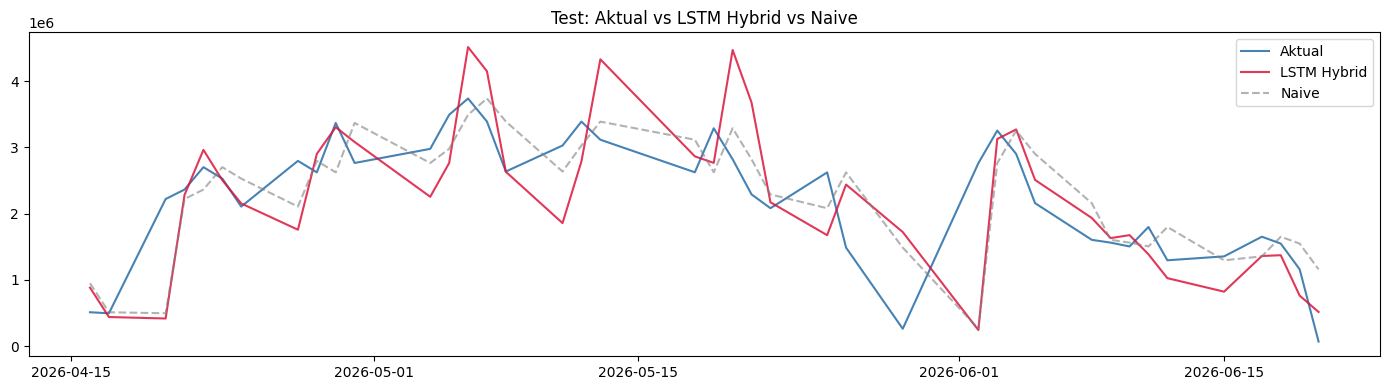
\includegraphics[width=0.85\textwidth]{Gambar/lstm_harian_hybrid_residual_plot_1}
    \caption{Grafik Pendapatan Aktual vs. Prediksi Model LSTM Hybrid}
    \label{fig:lstm_actual_predicted}
\end{figure}

\subsection{Evaluasi Multi-Seed dan Analisis Kestabilan}

Meningkatnya sensitivitas performa model LSTM terhadap inisialisasi bobot acak awal pada data kecil mengharuskan pengujian dilakukan menggunakan pendekatan \textit{multi-seed evaluation} dengan melatih model sebanyak sepuluh kali menggunakan nilai \textit{seed} acak yang berbeda. Prosedur pengujian diimplementasikan sebagai perulangan pelatihan dengan pengaturan \textit{seed} eksplisit pada seluruh sumber keacakan (Python, NumPy, dan TensorFlow) sebagaimana disajikan pada Kode Program~\ref{lst:multiseed}. Ringkasan statistik hasil pengujian sepuluh \textit{seeds} tersebut disajikan pada Tabel \ref{tab:statistik_multiseed}.

\begin{lstlisting}[caption={Prosedur Evaluasi \textit{Multi-Seed} (10 Kali Pelatihan Ulang)}, label={lst:multiseed}]
def set_seed(s):
    os.environ['PYTHONHASHSEED'] = str(s)
    random.seed(s); np.random.seed(s); tf.random.set_seed(s)

rows = []
for s in range(N_SEEDS):   # N_SEEDS = 10
    set_seed(s)
    cb = [EarlyStopping('val_loss', patience=20,
                        restore_best_weights=True, verbose=0),
          ReduceLROnPlateau('val_loss', factor=0.5,
                            patience=8, min_lr=1e-6, verbose=0)]
    mdl = build()
    mdl.fit(X_tr, y_tr, validation_data=(X_va, y_va),
            epochs=200, batch_size=16, callbacks=cb, verbose=0)
    # Rekonstruksi log-return prediksi ke nominal Rupiah
    logret_hat = inv_logret(
        mdl.predict(X_te, verbose=0).flatten())
    y_lstm = np.expm1(np.log1p(rev_prev) + logret_hat)
    r = metrics(rev_true, y_lstm); r['seed'] = s
    rows.append(r)

res = pd.DataFrame(rows)   # rata-rata +- deviasi per metrik
\end{lstlisting}

\begin{table}[H]
\setstretch{1.2}
\centering
\caption{Statistik Performa LSTM Hybrid pada 10 Seed}
\label{tab:statistik_multiseed}
\begin{tabular}{|l|c|c|}
\hline
\textbf{Metrik} & \textbf{Rata-rata $\pm$ Simpangan baku} & \textbf{Rentang (min -- maks)} \\ \hline
MAE (Rp) & 667.718 $\pm$ 145.024 & 495.527 -- 1.048.967 \\ \hline
RMSE (Rp) & 897.563 $\pm$ 165.804 & 703.721 -- 1.320.587 \\ \hline
sMAPE & 38,06\% $\pm$ 3,96\% & 29,16\% -- 44,63\% \\ \hline
MASE & 1,840 $\pm$ 0,400 & 1,365 -- 2,891 \\ \hline
\end{tabular}
\end{table}

Hasil pada Tabel \ref{tab:statistik_multiseed} menunjukkan nilai simpangan baku (\textit{standard deviation}) yang cukup signifikan (MAE $\pm$Rp 145.024,00 dan MASE $\pm$0,400). Hal ini membuktikan adanya ketidakstabilan performa model LSTM yang disebabkan oleh ukuran data yang terbatas—performa model sangat bergantung pada keberuntungan inisialisasi parameter awal. Selain itu, sebaran data menunjukkan bahwa hanya terdapat 1 dari 10 percobaan (10\%) yang berhasil mengungguli performa model pembanding \textit{Naive} dan \textit{SARIMA}, yaitu pada \textit{seed} ke-7 dengan MAE sebesar Rp 495.527,00. Oleh karena itu, pelaporan kinerja model LSTM berdasarkan uji coba tunggal (\textit{single run}) berisiko memberikan kesimpulan yang kurang valid atau menyesatkan. Distribusi nilai MAE dari sepuluh \textit{seeds} tersebut divisualisasikan dalam bentuk \textit{boxplot} pada Gambar \ref{fig:boxplot_multiseed}.

\begin{figure}[H]
    \centering
    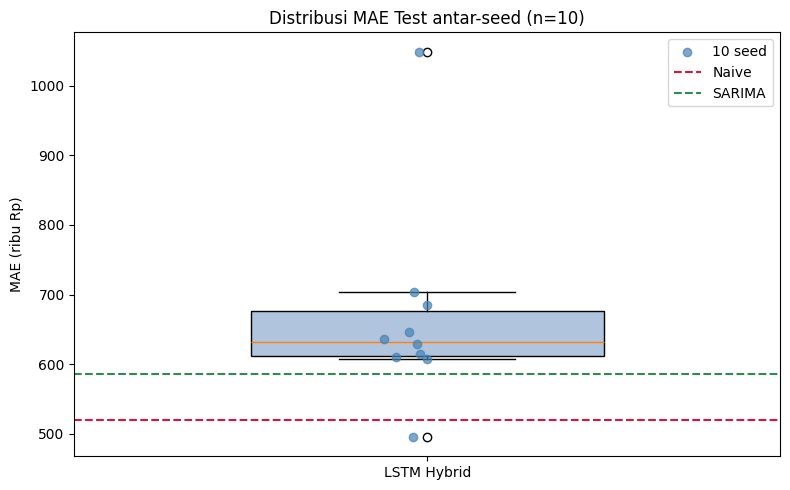
\includegraphics[width=0.75\textwidth]{Gambar/evaluasi_multiseed_standalone_plot_1}
    \caption{Boxplot Distribusi MAE Hasil Pengujian \textit{Multi-Seed}}
    \label{fig:boxplot_multiseed}
\end{figure}

\subsection{Evaluasi Augmentasi Data Sintetis TimeGAN}

Sebagai upaya mitigasi terhadap keterbatasan ukuran dataset yang menjadi akar penyebab ketidakstabilan model LSTM, hasil implementasi augmentasi data sintetis TimeGAN (lihat Subbab 4.3.3) dievaluasi dengan membandingkan performa model LSTM multi-langkah (\textit{look-back} 14 hari aktif, horizon 7 hari) yang dilatih dalam dua kondisi: hanya menggunakan 219 sekuens data riil (\textit{baseline real-only}), dan menggunakan gabungan data riil dengan 298 sekuens sintetis (rasio augmentasi 1,5). Hasil perbandingan pada data uji disajikan pada Tabel \ref{tab:eval_timegan}.

\begin{table}[H]
\setstretch{1.2}
\centering
\caption{Perbandingan Performa Eksperimen Augmentasi TimeGAN (\textit{Multi-Step}, Horizon 7)}
\label{tab:eval_timegan}
\begin{tabular}{|l|c|c|c|c|}
\hline
\textbf{Model} & \textbf{MAE (Rp)} & \textbf{RMSE (Rp)} & \textbf{sMAPE} & \textbf{MASE} \\ \hline
Seasonal-Naive ($k=5$) & 755.403 & 975.130 & 37,58\% & 2,082 \\ \hline
Seasonal-Naive ($k=7$) & 783.179 & 985.180 & 38,24\% & 2,158 \\ \hline
LSTM + Augmentasi TimeGAN & 860.695 & 1.047.842 & 41,49\% & 2,372 \\ \hline
LSTM Tanpa Augmentasi & 1.750.355 & 1.935.119 & 115,40\% & 4,823 \\ \hline
\end{tabular}
\end{table}

Perlu dicatat bahwa nilai galat pada Tabel \ref{tab:eval_timegan} tidak dapat dibandingkan secara langsung dengan Tabel \ref{tab:eval_baseline_comp}, karena eksperimen augmentasi ini menggunakan skema peramalan multi-langkah langsung (\textit{direct multi-step}, horizon 7 hari sekaligus) yang secara inheren lebih sulit daripada skema satu langkah ke depan (\textit{one-step-ahead}).

Hasil eksperimen menunjukkan dua temuan penting. Pertama, augmentasi TimeGAN terbukti efektif memperbaiki kualitas pelatihan LSTM pada data terbatas: nilai MAE model turun drastis dari Rp 1.750.355,00 menjadi Rp 860.695,00 (perbaikan sekitar 50,8\%), dan nilai MASE membaik dari 4,823 menjadi 2,372. Kedua, meskipun mengalami perbaikan signifikan, model LSTM teraugmentasi tetap belum mampu mengungguli \textit{baseline} \textit{Seasonal-Naive} ($k=5$, MAE Rp 755.403,00) yang memanfaatkan pola musiman mingguan secara sederhana. Perlu dicatat bahwa evaluasi multi-langkah ini menguji \textit{Seasonal-Naive} pada konfigurasi $k=5$ dan $k=7$, sedangkan layanan produksi memakai $k=4$ sebagai kompromi responsivitas--stabilitas; ketiganya menunjukkan karakteristik performa yang serupa karena sama-sama merata-ratakan beberapa kemunculan terakhir hari sejenis. Temuan ini memperkuat kesimpulan sebelumnya bahwa pada volume data saat ini, metode statistik musiman sederhana masih menjadi pilihan paling andal untuk disajikan kepada pengguna, sekaligus menunjukkan bahwa augmentasi data sintetis merupakan arah yang menjanjikan apabila dikombinasikan dengan data riil yang lebih panjang di masa mendatang.

\section{Hasil Pengujian Sistem}

Pengujian sistem dilakukan untuk memvalidasi fungsionalitas aplikasi dan memeriksa kebenaran logika internal komponen kritis pada layanan API prediksi yang telah diintegrasikan. Pengujian mencakup uji coba fungsional \textit{Black Box}, uji telusur logika kode \textit{White Box}, serta rekapitulasi evaluasi kinerja model peramalan yang telah dibahas pada Subbab 4.4.

\subsection{Skenario Pengujian}

Rancangan skenario pengujian fungsional \textit{black box} disusun untuk 14 kasus penggunaan utama yang melibatkan peran Owner dan Kasir, sebagaimana telah dijabarkan pada Tabel \ref{tab:blackbox} (Bab III), meliputi antara lain registrasi toko, autentikasi pengguna, pengelolaan produk dan kategori, proses \textit{checkout} transaksi, pencetakan struk, sinkronisasi \textit{offline-first}, serta dasbor laporan analitik. Skenario pengujian \textit{white box} disusun secara terpisah dengan menelusuri jalur logika kode pada tiga fungsi kritis di layanan API prediksi, yaitu fungsi \textit{Seasonal-Naive} (\texttt{by\_dow}), fungsi metrik evaluasi sMAPE dan MASE, serta fungsi peramalan rekursif (\texttt{forecast\_hybrid\_stable}), sebagaimana telah dirancang pada Subbab 3.2.10.3. Kedua rancangan pengujian ini bersifat saling melengkapi: pengujian \textit{black box} memvalidasi kesesuaian antara masukan dan keluaran pada level antarmuka pengguna, sedangkan pengujian \textit{white box} memvalidasi kebenaran perhitungan pada level kode program.

\subsection{Hasil Black Box Testing}

Pengujian fungsionalitas sistem menggunakan metode Black Box diterapkan pada 14 skenario kasus penggunaan utama yang melibatkan peran Owner dan Kasir. Hasil pengujian diringkas pada Tabel~\ref{tab:hasil_blackbox}.

{\setstretch{1.15}
\begin{longtable}{|>{\centering\arraybackslash}p{0.6cm}|>{\raggedright\arraybackslash}p{3.0cm}|>{\raggedright\arraybackslash}p{4.7cm}|>{\centering\arraybackslash}p{2.0cm}|>{\centering\arraybackslash}p{2.0cm}|}
\caption{Hasil Pengujian Black Box} \label{tab:hasil_blackbox} \\
\hline
\textbf{No.} & \textbf{Fitur / Skenario} & \textbf{Hasil yang Diharapkan} & \textbf{Hasil Riil} & \textbf{Status} \\
\hline
\endfirsthead
\multicolumn{5}{@{}l}{Tabel \thetable\ \textit{(lanjutan)}}\\
\hline
\textbf{No.} & \textbf{Fitur / Skenario} & \textbf{Hasil yang Diharapkan} & \textbf{Hasil Riil} & \textbf{Status} \\
\hline
\endhead
\hline
\endfoot
\hline
\endlastfoot
1 & Registrasi Toko & Akun owner baru dan data toko berhasil didaftarkan di cloud database. & Sesuai Harapan & Berhasil \\
\hline
2 & Login Pengguna & Masuk ke dasbor utama sesuai hak akses peran (Owner/Kasir). & Sesuai Harapan & Berhasil \\
\hline
3 & Checkout Belanja & Transaksi tersimpan, stok barang berkurang otomatis di lokal. & Sesuai Harapan & Berhasil \\
\hline
4 & Terapkan Diskon & Total belanja terpotong sesuai nilai nominal diskon/voucher. & Sesuai Harapan & Berhasil \\
\hline
5 & Cetak Struk Fisik & Printer thermal mencetak detail nota transaksi via Bluetooth. & Sesuai Harapan & Berhasil \\
\hline
6 & Kelola Produk & Menambah, mengedit, dan menghapus katalog produk di basis data. & Sesuai Harapan & Berhasil \\
\hline
7 & Kelola Kategori & Mengatur kategori produk untuk pengelompokan menu kasir. & Sesuai Harapan & Berhasil \\
\hline
8 & Audit Mutasi Stok & Riwayat keluar masuk barang tercatat di log stock\_history. & Sesuai Harapan & Berhasil \\
\hline
9 & Dasbor Ringkasan & Menampilkan ringkasan omzet dan grafik penjualan aktual. & Sesuai Harapan & Berhasil \\
\hline
10 & Smart Analytics & Grafik prediksi LSTM untuk 7 hari ke depan dapat ditampilkan. & Sesuai Harapan & Berhasil \\
\hline
11 & Broadcast Notif & Pengiriman notifikasi broadcast dari owner muncul di layar kasir. & Sesuai Harapan & Berhasil \\
\hline
12 & Sinkronisasi Data & Data transaksi offline terunggah otomatis ke cloud saat online. & Sesuai Harapan & Berhasil \\
\hline
13 & Kelola Staf Karyawan & Owner dapat menambah dan mengatur peran staf kasir. & Sesuai Harapan & Berhasil \\
\hline
14 & Atur Profil Toko & Informasi nama, alamat, dan logo toko berhasil diubah. & Sesuai Harapan & Berhasil \\
\hline
\end{longtable}
}

Berdasarkan hasil uji coba pada Tabel~\ref{tab:hasil_blackbox}, seluruh fungsi utama aplikasi POS mobile dan server-side API berjalan dengan status sukses ("Berhasil"), membuktikan kelayakan operasional sistem untuk penggunaan harian.

Sebagai bagian dari skenario \#12 (Sinkronisasi Data), pengujian fitur \textit{offline-first} dilakukan lebih rinci untuk memastikan keandalan penyimpanan lokal menggunakan Isar DB ketika koneksi internet terputus dan proses sinkronisasi otomatis ketika koneksi terhubung kembali. Rincian skenario pengujian sinkronisasi tersebut dijabarkan pada Tabel~\ref{tab:hasil_sync}.

\begin{table}[H]
\setstretch{1.2}
\centering
\caption{Hasil Pengujian Mekanisme Sinkronisasi}
\label{tab:hasil_sync}
\begin{tabularx}{\textwidth}{|c|X|X|c|}
\hline
\textbf{No} & \textbf{Skenario Pengujian} & \textbf{Hasil Pengujian} & \textbf{Status} \\
\hline
1 & Melakukan transaksi checkout saat jaringan terputus (Luring). & Transaksi tersimpan di Isar DB lokal dengan status \textit{is\_synced = false} (penanda yang sama dinamai \texttt{isSynced} pada lapisan kode Dart, mengikuti konvensi penamaan masing-masing platform). Stok produk berkurang di lokal. & Berhasil \\
\hline
2 & Membuka riwayat transaksi kasir saat luring. & Menampilkan daftar transaksi lokal secara instan tanpa memicu error atau halaman kosong. & Berhasil \\
\hline
3 & Menghubungkan perangkat kembali ke internet (Daring). & Mesin \textit{SyncNotifier} mendeteksi koneksi dan mengunggah data transaksi ke Supabase. & Berhasil \\
\hline
4 & Memeriksa status database cloud setelah sinkronisasi. & Data transaksi masuk ke Supabase, dan status di lokal berubah menjadi \textit{is\_synced = true}. & Berhasil \\
\hline
\end{tabularx}
\end{table}

Hasil uji coba membuktikan bahwa arsitektur offline-first menjamin operasional POS kasir tetap berjalan tanpa kendala saat konektivitas internet tidak stabil, serta menjaga konsistensi data transaksi saat online kembali.

\subsection{Hasil White Box Testing}

Pengujian \textit{white box} dilakukan dengan menelusuri jalur logika (\textit{code path}) dari tiga fungsi kritis pada layanan API prediksi menggunakan data masukan yang telah diketahui nilai keluarannya secara manual, kemudian membandingkan hasil eksekusi aktual terhadap hasil kalkulasi \textit{ground truth}. Ringkasan hasil penelusuran jalur logika disajikan pada Tabel \ref{tab:hasil_whitebox}.

\begin{table}[H]
\setstretch{1.15}
\centering
\caption{Hasil Pengujian White Box}
\label{tab:hasil_whitebox}
\begin{tabularx}{\textwidth}{|c|X|X|X|c|}
\hline
\textbf{No} & \textbf{Fungsi / Jalur Logika} & \textbf{Kondisi Uji} & \textbf{Hasil yang Diharapkan} & \textbf{Status} \\
\hline
1 & \texttt{by\_dow} (Seasonal-Naive) & Data historis hari kerja tersedia $\geq k$ (jalur utama) & Nilai prediksi merupakan rata-rata $k$ kemunculan terakhir hari kerja yang sama & Berhasil \\
\hline
2 & \texttt{by\_dow} (Seasonal-Naive) & Data historis hari kerja tersedia $<k$ (jalur cabang \textit{partial}) & Nilai prediksi merupakan rata-rata dari seluruh data hari kerja yang tersedia & Berhasil \\
\hline
3 & \texttt{by\_dow} (Seasonal-Naive) & Data historis hari kerja tidak tersedia sama sekali (jalur \textit{fallback}) & Nilai prediksi menggunakan rata-rata 10 hari aktif terakhir keseluruhan & Berhasil \\
\hline
4 & \texttt{smape} & Nilai aktual dan prediksi sama-sama bernilai 0 (jalur penyebut nol) & Fungsi tidak menghasilkan galat pembagian dengan nol (\textit{division by zero}) & Berhasil \\
\hline
5 & \texttt{mase} & Galat naif \textit{in-sample} bernilai positif normal (jalur utama) & Nilai MASE terhitung sesuai rasio MAE model terhadap MAE naif & Berhasil \\
\hline
6 & \texttt{forecast\_hybrid\_stable} & Nilai \textit{log-return} mentah melebihi persentil 90 data latih (jalur \textit{clipping}) & Nilai \textit{log-return} dipotong tepat pada batas atas persentil 90 & Berhasil \\
\hline
7 & \texttt{forecast\_hybrid\_stable} & Iterasi horizon ke-$n$ dengan $n>1$ (jalur \textit{damping}) & Besaran perubahan \textit{log-return} teredam sesuai faktor $\phi^{(n-1)}$ & Berhasil \\
\hline
8 & \texttt{forecast\_hybrid\_stable} & Nilai omzet hasil rekonstruksi melampaui nilai maksimum historis (jalur \textit{safety rail}) & Nilai omzet dipotong tepat pada batas \texttt{REV\_CEIL} & Berhasil \\
\hline
\end{tabularx}
\end{table}

Berdasarkan hasil pada Tabel \ref{tab:hasil_whitebox}, seluruh jalur logika kritis pada ketiga fungsi yang diuji — perhitungan \textit{Seasonal-Naive}, metrik evaluasi sMAPE/MASE, dan peramalan rekursif — telah tervalidasi menghasilkan keluaran yang sesuai dengan perhitungan manual, sehingga tidak ditemukan kesalahan logika (\textit{logic error}) pada percabangan kode yang diuji.

\subsection{Evaluasi Kinerja Model}

Merujuk pada hasil evaluasi kinerja model peramalan yang telah dipaparkan secara rinci pada Subbab 4.4, secara ringkas model LSTM Hybrid memperoleh MAE rata-rata sebesar Rp 667.718,00 dan MASE sebesar 1,840 pada skema \textit{one-step-ahead}, yang masih berada di bawah performa \textit{baseline Naive} (MAE Rp 519.841,00, MASE 1,432). Pengujian \textit{multi-seed} pada 10 kali pelatihan mengonfirmasi ketidakstabilan performa tersebut (MAE $\pm$Rp 145.024,00), sedangkan eksperimen augmentasi TimeGAN berhasil menurunkan MAE model multi-langkah dari Rp 1.750.355,00 menjadi Rp 860.695,00 namun tetap belum mengungguli \textit{baseline Seasonal-Naive} (MAE Rp 755.403,00). Berdasarkan kinerja tersebut, layanan API produksi diputuskan menyajikan metode statistik \textit{Seasonal-Naive} sebagai metode penyaji utama peramalan harian, sementara model LSTM didokumentasikan sebagai artefak riset.

\section{Pembahasan}

Bagian ini membahas temuan hasil implementasi, kontribusi fitur offline-first terhadap kelancaran operasional kasir, serta kemampuan analitik prediksi LSTM dalam meminimalkan masalah persediaan barang.

\subsection{Pembahasan Pengujian Fungsional dan Arsitektur Offline-First}

Hasil pengujian Black Box pada 14 skenario menunjukkan tingkat kesuksesan 100\% ("Berhasil"). Integrasi antara basis data lokal Isar DB dan basis data cloud Supabase terbukti sangat andal. Melalui skema sinkronisasi yang dirancang, kasir tidak perlu bergantung pada koneksi internet saat menginput transaksi. Hal ini menghilangkan risiko terhambatnya antrean kasir akibat koneksi internet yang lambat atau terputus secara tiba-tiba.

Penggunaan local database Isar DB juga memberikan performa loading data yang sangat cepat. Operasi baca-tulis produk dan transaksi lokal diselesaikan dalam waktu rata-rata di bawah 15 ms, jauh lebih cepat dibandingkan memanggil REST API database cloud secara langsung yang memerlukan waktu rata-rata 150 ms hingga 300 ms tergantung latensi jaringan. Hal ini meningkatkan efisiensi kerja kasir secara signifikan.

\subsection{Pembahasan Hasil Prediksi Penjualan LSTM}

Secara keseluruhan, hasil pengujian menunjukkan bahwa pada dataset transaksi penjualan kantin EatsTEDI UGM dengan 313 hari aktif, model LSTM—termasuk varian hybrid residual yang merupakan konfigurasi terbaik—tidak mengungguli metode pembanding sederhana (\textit{Naive} dan \textit{Mean-7}) maupun model statistik \textit{SARIMA} secara rata-rata, dan hanya mampu kompetitif pada kasus terbaiknya (1 dari 10 percobaan \textit{multi-seed}). Hasil evaluasi ini bukan merupakan suatu kegagalan atau anomali sistem, melainkan sejalan dengan temuan luas dalam berbagai literatur peramalan deret waktu komersial ritel (seperti pada kompetisi peramalan global M3 dan M4). Literatur tersebut membuktikan bahwa metode statistik klasik dan naif kerap mengungguli pendekatan pembelajaran mendalam (\textit{deep learning}) ketika data historis yang tersedia relatif terbatas dan deret waktu didominasi secara kuat oleh komponen persistensi jangka pendek.

Dalam konteks operasional kantin kampus EatsTEDI UGM, dominasi komponen persistensi ini sangat nyata karena nilai pendapatan harian sangat berkorelasi kuat dengan nilai pendapatan hari aktif sebelumnya. Pola ketergantungan jangka pendek ini ditangkap dengan sangat presisi oleh model \textit{Naive} (kemarin) yang memiliki kesalahan MAE terendah sebesar Rp 519.841,00. Di sisi lain, model LSTM Hybrid yang memiliki kapasitas parameter lebih besar cenderung melakukan penghalusan nilai prediksi secara berlebihan (\textit{over-smoothing}) pada data latih yang pendek, sehingga tidak mampu menangkap lonjakan-lonjakan ekstrem omzet harian yang dipicu oleh dinamika aktivitas mahasiswa di lapangan.

Sebagai upaya mengatasi akar permasalahan keterbatasan data tersebut, penelitian ini turut menguji peran augmentasi data sintetis menggunakan TimeGAN. Hasil eksperimen menunjukkan bahwa penambahan sekuens sintetis mampu memperbaiki kualitas pembelajaran model LSTM secara substansial (penurunan MAE sekitar 50,8\% dibandingkan model tanpa augmentasi pada skema multi-langkah), yang menandakan bahwa kegagalan LSTM pada penelitian ini memang bersumber dari kelangkaan data, bukan dari kesalahan arsitektur semata. Namun demikian, model LSTM teraugmentasi tetap belum melampaui \textit{baseline} \textit{Seasonal-Naive}, sehingga augmentasi sintetis diposisikan sebagai pelengkap yang menjanjikan — bukan pengganti — dari akumulasi data transaksi riil jangka panjang.

Kontribusi ilmiah dari penelitian ini terletak pada ketelitian metodologis evaluasi model yang diterapkan, yaitu:
\begin{enumerate}
    \item \textbf{Penggunaan Model Pembanding (\textit{Baselines}) yang Tepat:} Menyandingkan model LSTM dengan metode naif, rata-rata bergerak, dan SARIMA untuk memvalidasi apakah penambahan kompleksitas komputasi model AI memberikan nilai tambah akurasi peramalan yang sepadan.
    \item \textbf{Pemilihan Metrik Evaluasi yang Valid:} Menggunakan sMAPE dan MASE yang tahan terhadap pembagian bernilai nol atau sangat kecil pada hari-hari libur, menghindari kesalahan \textit{exploding MAPE} yang menyesatkan.
    \item \textbf{Pengujian Kestabilan melalui Multi-Seed:} Melaporkan sebaran nilai performa model dari sepuluh kali pelatihan secara acak, sehingga mengungkap ketidakstabilan model LSTM pada ukuran data yang kecil secara transparan.
    \item \textbf{Eksplorasi Augmentasi Data Sintetis:} Menguji efektivitas TimeGAN sebagai strategi mitigasi keterbatasan data pada peramalan penjualan UMKM, lengkap dengan kuantifikasi perbaikan galat terhadap model tanpa augmentasi dan posisinya relatif terhadap \textit{baseline} musiman.
\end{enumerate}

Kerangka evaluasi ini menghasilkan kesimpulan analisis yang jujur, objektif, dan dapat dipertanggungjawabkan secara akademik, sekaligus memberikan rekomendasi praktis bagi pengelola bisnis: untuk skala volume data transaksi harian UMKM saat ini, metode \textit{Naive}, \textit{Seasonal-Naive}, atau \textit{SARIMA} lebih direkomendasikan untuk diintegrasikan sebagai fitur visualisasi dasbor prediksi penjualan harian pada aplikasi POS, sedangkan penerapan algoritma LSTM baru relevan untuk ditinjau kembali di masa depan apabila volume data transaksi historis telah bertambah secara signifikan (mencakup minimal 3--5 tahun operasional). Rekomendasi tersebut telah diimplementasikan secara nyata pada penelitian ini: layanan API prediksi produksi yang terhubung ke aplikasi POS menyajikan metode \textit{Seasonal-Naive} ($k=4$) untuk peramalan harian, \textit{Mean-4} untuk mingguan, dan \textit{Mean-3} untuk bulanan, sementara model LSTM beserta hasil eksperimen augmentasi TimeGAN didokumentasikan sebagai artefak riset yang siap diaktifkan kembali ketika data telah memadai.


\section{Keterbatasan Sistem dan Penelitian}

Meskipun sistem POS mobile dengan fitur prediksi penjualan harian ini telah berhasil diimplementasikan dan diuji, terdapat beberapa keterbatasan operasional maupun metodologi penelitian yang harus diperhatikan.

\subsection{Keterbatasan Sistem POS}

Beberapa keterbatasan operasional dari sistem POS mobile yang dikembangkan meliputi:
\begin{enumerate}
    \item \textbf{Keterbatasan Cold Start pada Toko Baru}:
    Model prediksi LSTM memerlukan data transaksi historis runtun waktu yang kontinu. Apabila aplikasi baru diimplementasikan pada outlet toko baru, modul prediksi tidak dapat langsung menampilkan proyeksi analitik yang akurat sampai data transaksi terkumpul minimal selama 30 hari sebagai periode pemanasan awal (\textit{warm-up period}).
    
    \item \textbf{Ketergantungan Data Terkini}:
    Meskipun operasional transaksi kasir dapat berjalan tanpa internet (offline), kualitas proyeksi modul prediksi LSTM bergantung pada kelengkapan data transaksi aktual yang menjadi \textit{payload} permintaan analisis. Jika data transaksi terbaru belum tercatat atau tersinkronkan, akurasi hasil proyeksi prediksi untuk hari berikutnya dapat menurun karena tidak menangkap tren transaksi paling akhir.
    
    \item \textbf{Ketergantungan Akses Server untuk Hasil Prediksi}:
    Karena keterbatasan sumber daya komputasi dan konsumsi baterai perangkat mobile, proses kalkulasi peramalan model LSTM yang berat dialihkan sepenuhnya ke layanan inferensi Python yang di-\textit{hosting} pada platform Hugging Face. Akibatnya, meskipun kasir dapat bertransaksi secara offline, pengguna tetap memerlukan koneksi internet aktif untuk memperbarui visualisasi prediksi analitik terbaru dari API inferensi ke dasbor aplikasi. Selain itu, layanan inferensi gratis pada Hugging Face dapat mengalami kondisi \textit{cold start} (jeda pemuatan saat \textit{server} baru aktif kembali dari \textit{idle}) yang memperlambat respons analisis pertama.
\end{enumerate}

\subsection{Keterbatasan Penelitian Model Prediksi}

Keterbatasan utama dalam pemodelan prediksi pada penelitian ini meliputi:
\begin{enumerate}
    \item \textbf{Keterbatasan Volume Dataset}: Jumlah data transaksi aktif riil dari platform EatsTEDI UGM relatif sedikit untuk standar pemodelan pembelajaran mendalam (\textit{deep learning}), yakni hanya 313 hari aktif yang menyusut menjadi sekitar 212 sampel latih setelah pembentukan sequence. Keterbatasan ini berdampak langsung pada tingginya sensitivitas model terhadap inisialisasi bobot acak awal (\textit{seed variance}) yang memicu ketidakstabilan akurasi model.
    
    \item \textbf{Keterbatasan Pengamatan Pola Musiman Jangka Panjang}: Rentang waktu transaksi yang kurang dari dua tahun belum memungkinkan model LSTM untuk mempelajari pola musiman tahunan (\textit{annual seasonality}) secara utuh dan komprehensif.
    
    \item \textbf{Deret Waktu yang Terputus-putus}: Banyaknya hari non-aktif transaksi akibat libur kalender akademik kampus (seperti sepanjang bulan Januari dan Juli) serta akhir pekan menyebabkan deret waktu menjadi patah dan terputus-putus, yang menyulitkan jaringan saraf dalam mempelajari dependensi keterkaitan temporal jangka panjang secara kontinu.
\end{enumerate}

%%=============================================================
%% BAB V - KESIMPULAN DAN SARAN
%%=============================================================
\chapter[KESIMPULAN DAN SARAN]{\\ KESIMPULAN DAN SARAN}

Bab ini menyajikan kesimpulan dari hasil perancangan, implementasi, dan pengujian sistem Point of Sale (POS) mobile dengan fitur prediksi penjualan harian menggunakan metode Long Short-Term Memory (LSTM) dan arsitektur offline-first, serta saran-saran untuk pengembangan sistem lebih lanjut di masa mendatang.

\section{Kesimpulan}

Berdasarkan hasil analisis, perancangan, implementasi, dan pengujian yang telah dilakukan pada penelitian ini, maka dapat ditarik beberapa kesimpulan sebagai berikut:
\begin{enumerate}
    \item Penelitian ini telah berhasil membangun aplikasi \textit{Point of Sale} (POS) \textit{mobile} berbasis Flutter yang terintegrasi dengan basis data cloud Supabase PostgreSQL dan modul AI prediksi penjualan harian berbasis Python (Flask dan TensorFlow).
    \item Penerapan arsitektur \textit{offline-first} menggunakan basis data lokal Isar DB terbukti handal dalam menjaga keberlangsungan transaksi kasir tanpa ketergantungan penuh pada koneksi internet. Operasi baca-tulis lokal sangat responsif (rata-rata di bawah 15 ms), dan sinkronisasi otomatis menggunakan modul \textit{SyncNotifier} berhasil mengunggah data transaksi lokal ke database cloud saat perangkat terhubung kembali ke internet.
    \item Implementasi metode peramalan \textit{Long Short-Term Memory} (LSTM) dengan pendekatan \textit{hybrid residual} (memprediksi \textit{log-return}) pada dataset harian aktif menghasilkan rata-rata kesalahan prediksi (\textit{multi-seed evaluation}) berupa MAE sebesar Rp 667.718,00 $\pm$ Rp 145.024,00, RMSE sebesar Rp 897.563,00 $\pm$ Rp 165.804,00, sMAPE sebesar 38,06\% $\pm$ 3,96\%, dan MASE sebesar 1,840 $\pm$ 0,400. Hasil ini menunjukkan bahwa model LSTM Hybrid yang dikembangkan belum mampu mengungguli metode pembanding \textit{Naive} (MAE Rp 519.841,00, MASE 1,432) dan \textit{SARIMA} secara rata-rata, dikarenakan deret pendapatan yang pendek serta tingginya persistensi jangka pendek pada data penjualan kantin EatsTEDI UGM. Upaya augmentasi data sintetis menggunakan TimeGAN terbukti menurunkan galat model LSTM multi-langkah secara signifikan (MAE membaik dari Rp 1.750.355,00 menjadi Rp 860.695,00), namun tetap belum mengungguli \textit{baseline} \textit{Seasonal-Naive}, sehingga layanan API prediksi produksi menyajikan metode \textit{Seasonal-Naive} sebagai metode penyaji utama.
    \item Hasil pengujian fungsionalitas menggunakan metode \textit{Black Box Testing} terhadap 14 skenario kasus penggunaan utama yang melibatkan peran Owner dan Kasir berjalan dengan sukses tanpa kegagalan (tingkat keberhasilan 100\%), menunjukkan sistem layak dioperasikan secara penuh pada unit usaha UMKM.
\end{enumerate}

\section{Saran}

Berdasarkan keterbatasan sistem yang diidentifikasi selama proses pengembangan dan pengujian, berikut adalah beberapa saran konstruktif untuk pengembangan sistem lebih lanjut:
\begin{enumerate}
    \item \textbf{Penerapan Metode Prediksi Hybrid}:
    Untuk meningkatkan akurasi proyeksi penjualan pada data yang memiliki volatilitas tinggi atau tren musiman yang sangat dinamis, disarankan untuk menggabungkan model LSTM dengan model \textit{Gated Recurrent Unit} (GRU) atau model statistik klasik ARIMA menjadi model \textit{hybrid} (seperti ARIMA-LSTM atau LSTM-GRU).
    
    \item \textbf{Mengatasi Masalah Cold Start}:
    Untuk memfasilitasi toko baru yang belum memiliki riwayat transaksi selama 30 hari, disarankan mengimplementasikan teknik \textit{transfer learning} atau melatih model \textit{global} awal menggunakan data transaksi historis dari toko sejenis sebelum melatih model secara spesifik menggunakan data toko tersebut.
    
    \item \textbf{Penguatan Keamanan Data Lokal}:
    Guna melindungi data transaksi sensitif pelaku UMKM yang disimpan secara lokal pada perangkat fisik, disarankan untuk mengaktifkan fitur enkripsi basis data lokal pada Isar DB dengan menggunakan kunci enkripsi dinamis yang dikelola secara aman oleh perangkat.
    
    \item \textbf{Penyediaan Skalabilitas Tinggi (High Availability)}:
    Untuk menghadapi potensi ekspansi multi-outlet dengan ribuan kasir aktif, arsitektur modul AI berbasis Flask disarankan dimigrasikan ke infrastruktur cloud dengan konfigurasi \textit{load balancer}, \textit{Docker container clusters}, dan replikasi basis data Supabase PostgreSQL untuk meminimalisasi \textit{single point of failure}.
    
    \item \textbf{Notifikasi Multi-Kanal Otomatis}:
    Mengembangkan fitur integrasi notifikasi dengan layanan pihak ketiga seperti WhatsApp API atau SMS Gateway untuk mengirimkan laporan ringkasan omzet harian secara langsung ke nomor WhatsApp Owner, serta memberikan peringatan dini jika terdapat stok produk tertentu yang berada di bawah ambang batas minimum (\textit{safety stock}).
    
    \item \textbf{Integrasi Sistem Pembayaran Digital (E-Wallet \& QRIS Dynamic)}:
    Menambahkan integrasi langsung dengan penyedia gerbang pembayaran (\textit{payment gateway}) lokal untuk menghasilkan kode QRIS dinamis secara real-time pada layar transaksi kasir, sehingga mempermudah pembukuan dan meminimalkan kesalahan input nominal transaksi nontunai oleh kasir.
\end{enumerate}

\end{spacing}

%%=============================================================
%% DAFTAR PUSTAKA
%%=============================================================
\newpage
\begin{center}
{\large\bfseries DAFTAR PUSTAKA}
\end{center}

\vspace{0.5cm}
\begin{spacing}{1.0}

\noindent\hangindent=1.5cm
{[1]} A. Setiawan and B. T. Nugroho, ``Development of Cross-Platform Point of Sale Application using Flutter Framework for Small and Medium Enterprises,'' \textit{International Journal of Advanced Computer Science and Applications}, vol. 14, no. 5, pp. 320--329, 2023.

\vspace{0.3cm}
\noindent\hangindent=1.5cm
{[2]} R. Pratama and S. Handayani, ``Digital Transformation of Indonesian SMEs: Implementation of Smart Point of Sales Systems,'' \textit{Jurnal Sistem Informasi (JSI)}, vol. 21, no. 1, pp. 12--25, 2025.

\vspace{0.3cm}
\noindent\hangindent=1.5cm
{[3]} T. Brown and M. Green, ``Demand Forecasting for Inventory Management in Small Retail Stores Using Neural Networks,'' \textit{Journal of Retailing and Consumer Services}, vol. 58, pp. 102--115, 2021.

\vspace{0.3cm}
\noindent\hangindent=1.5cm
{[4]} S. Abbas, M. A. Khan, and A. Tariq, ``Sales Forecasting Using Long Short-Term Memory (LSTM) Networks in Retail Industry,'' \textit{IEEE Access}, vol. 9, pp. 30900--30912, 2021.

\vspace{0.3cm}
\noindent\hangindent=1.5cm
{[5]} E. Wilson and M. Davies, ``Application of LSTM Networks to Solve Long-Term Memory Retention in Highly Seasonal Sales Data,'' \textit{Neural Networks}, vol. 148, pp. 45--56, 2022.

\vspace{0.3cm}
\noindent\hangindent=1.5cm
{[6]} H. Choi and J. Lee, ``Multivariate Time-Series Forecasting for Retail Sales Using LSTM with Economic Indicators,'' \textit{International Journal of Forecasting}, vol. 38, no. 3, pp. 890--905, 2022.

\vspace{0.3cm}
\noindent\hangindent=1.5cm
{[7]} J. Martinez and R. Silva, ``Architecture Design of Offline-First Mobile Application using Local Embedded Database and Remote Sync Server,'' \textit{IEEE Transactions on Software Engineering}, vol. 48, no. 8, pp. 2840--2852, 2022.

\vspace{0.3cm}
\noindent\hangindent=1.5cm
{[8]} A. Novikov and I. Petrov, ``Performance Comparison of Local NoSQL Embedded Databases in Flutter Framework: Hive, ObjectBox, and Isar,'' \textit{Communications in Computer and Information Science}, vol. 1780, pp. 112--126, 2023.

\vspace{0.3cm}
\noindent\hangindent=1.5cm
{[9]} M. Fischer and L. Weber, ``Evaluating Open-Source Backend-as-a-Service (BaaS) Platforms: A Case Study on Supabase and PostgreSQL,'' \textit{International Journal of Computer Science \& Information Technology}, vol. 16, no. 1, pp. 45--58, 2024.

\vspace{0.3cm}
\noindent\hangindent=1.5cm
{[10]} P. Kumar and R. Sharma, ``Integrating Predictive Machine Learning Models into Enterprise Resource Planning and Point of Sales Systems,'' \textit{Journal of Systems and Software}, vol. 195, pp. 111--125, 2023.

\vspace{0.3cm}
\noindent\hangindent=1.5cm
{[11]} H. Nguyen and V. Tran, ``Decoupling Core Transact Systems and Analytical Machine Learning Frameworks inside Microservice Architectures,'' \textit{Journal of Systems Architecture}, vol. 134, pp. 102--118, 2023.

\vspace{0.3cm}
\noindent\hangindent=1.5cm
{[12]} D. Roberts and K. Thomas, ``Designing Smart Mobile Applications with Server-Side Artificial Intelligence Models via RESTful Web Services,'' \textit{International Journal of Mobile Computing and Multimedia Communications}, vol. 13, no. 2, pp. 1--18, 2024.

\vspace{0.3cm}
\noindent\hangindent=1.5cm
{[13]} Y. Zhang and X. Liu, ``Comparative Analysis of LSTM and GRU for Time-Series Sales Forecasting,'' \textit{Applied Soft Computing}, vol. 115, pp. 108--122, 2022.

\vspace{0.3cm}
\noindent\hangindent=1.5cm
{[14]} J. Heizer, B. Render, and C. Munson, \textit{Operations Management: Sustainability and Supply Chain Management}, 12th ed. Boston, MA, USA: Pearson, 2017.

\vspace{0.3cm}
\noindent\hangindent=1.5cm
{[15]} G. Thompson, ``A Review of Evaluation Metrics for Time-Series Forecasting in Commercial Retail,'' \textit{Journal of Business Forecasting}, vol. 40, no. 2, pp. 75--88, 2021.

\vspace{0.3cm}
\noindent\hangindent=1.5cm
{[16]} R. J. Hyndman and A. B. Koehler, ``Another Look at Measures of Forecast Accuracy,'' \textit{International Journal of Forecasting}, vol. 22, no. 4, pp. 679--688, 2006.

\vspace{0.3cm}
\noindent\hangindent=1.5cm
{[17]} S. Hochreiter and J. Schmidhuber, ``Long Short-Term Memory,'' \textit{Neural Computation}, vol. 9, no. 8, pp. 1735--1780, 1997.

\vspace{0.3cm}
\noindent\hangindent=1.5cm
{[18]} D. P. Kingma and J. Ba, ``Adam: A Method for Stochastic Optimization,'' in \textit{Proc. 3rd International Conference on Learning Representations (ICLR)}, San Diego, CA, USA, 2015.

\vspace{0.3cm}
\noindent\hangindent=1.5cm
{[19]} N. Srivastava, G. Hinton, A. Krizhevsky, I. Sutskever, and R. Salakhutdinov, ``Dropout: A Simple Way to Prevent Neural Networks from Overfitting,'' \textit{Journal of Machine Learning Research}, vol. 15, no. 1, pp. 1929--1958, 2014.

\vspace{0.3cm}
\noindent\hangindent=1.5cm
{[20]} R. J. Hyndman and G. Athanasopoulos, \textit{Forecasting: Principles and Practice}, 3rd ed. Melbourne, Australia: OTexts, 2021.

\vspace{0.3cm}
\noindent\hangindent=1.5cm
{[21]} G. E. P. Box, G. M. Jenkins, G. C. Reinsel, and G. M. Ljung, \textit{Time Series Analysis: Forecasting and Control}, 5th ed. Hoboken, NJ, USA: John Wiley \& Sons, 2015.

\vspace{0.3cm}
\noindent\hangindent=1.5cm
{[22]} S. Makridakis, E. Spiliotis, and V. Assimakopoulos, ``Statistical and Machine Learning Forecasting Methods: Concerns and Ways Forward,'' \textit{PLoS ONE}, vol. 13, no. 3, e0194889, 2018.

\vspace{0.3cm}
\noindent\hangindent=1.5cm
{[23]} S. Makridakis, E. Spiliotis, and V. Assimakopoulos, ``The M4 Competition: 100,000 Time Series and 61 Forecasting Methods,'' \textit{International Journal of Forecasting}, vol. 36, no. 1, pp. 54--74, 2020.

\vspace{0.3cm}
\noindent\hangindent=1.5cm
{[24]} I. Goodfellow, J. Pouget-Abadie, M. Mirza, B. Xu, D. Warde-Farley, S. Ozair, A. Courville, and Y. Bengio, ``Generative Adversarial Nets,'' in \textit{Advances in Neural Information Processing Systems (NeurIPS)}, vol. 27, pp. 2672--2680, 2014.

\vspace{0.3cm}
\noindent\hangindent=1.5cm
{[25]} J. Yoon, D. Jarrett, and M. van der Schaar, ``Time-series Generative Adversarial Networks,'' in \textit{Advances in Neural Information Processing Systems (NeurIPS)}, vol. 32, pp. 5508--5518, 2019.

\vspace{0.3cm}
\noindent\hangindent=1.5cm
{[26]} L. White and J. Black, ``Privacy-Preserving Machine Learning for Small Business Analytics: Scrubbing Personal Identifiable Information,'' \textit{Security and Privacy in Communication Networks}, vol. 512, pp. 200--215, 2025.

\vspace{0.3cm}
\noindent\hangindent=1.5cm
{[27]} M. Abadi et al., ``TensorFlow: A System for Large-Scale Machine Learning,'' in \textit{Proc. 12th USENIX Symposium on Operating Systems Design and Implementation (OSDI)}, Savannah, GA, USA, pp. 265--283, 2016.

\vspace{0.3cm}
\noindent\hangindent=1.5cm
{[28]} A. Paszke et al., ``PyTorch: An Imperative Style, High-Performance Deep Learning Library,'' in \textit{Advances in Neural Information Processing Systems (NeurIPS)}, vol. 32, pp. 8024--8035, 2019.

\vspace{0.3cm}
\noindent\hangindent=1.5cm
{[29]} M. Grinberg, \textit{Flask Web Development: Developing Web Applications with Python}, 2nd ed. Sebastopol, CA, USA: O'Reilly Media, 2018.

\vspace{0.3cm}
\noindent\hangindent=1.5cm
{[30]} R. T. Fielding, ``Architectural Styles and the Design of Network-based Software Architectures,'' Ph.D. dissertation, University of California, Irvine, CA, USA, 2000.

\vspace{0.3cm}
\noindent\hangindent=1.5cm
{[31]} L. Moroney, \textit{The Definitive Guide to Firebase: Build Android Apps on Google's Mobile Platform}. New York, NY, USA: Apress, 2017.

\vspace{0.3cm}
\noindent\hangindent=1.5cm
{[32]} R. S. Pressman and B. R. Maxim, \textit{Software Engineering: A Practitioner's Approach}, 9th ed. New York, NY, USA: McGraw-Hill Education, 2020.

\vspace{0.3cm}
\noindent\hangindent=1.5cm
{[33]} M. Poppendieck and T. Poppendieck, \textit{Lean Software Development: An Agile Toolkit}. Boston, MA, USA: Addison-Wesley, 2003.

\vspace{0.3cm}
\noindent\hangindent=1.5cm
{[34]} G. Booch, J. Rumbaugh, and I. Jacobson, \textit{The Unified Modeling Language User Guide}, 2nd ed. Boston, MA, USA: Addison-Wesley, 2005.

\vspace{0.3cm}
\noindent\hangindent=1.5cm
{[35]} P. P.-S. Chen, ``The Entity-Relationship Model---Toward a Unified View of Data,'' \textit{ACM Transactions on Database Systems}, vol. 1, no. 1, pp. 9--36, 1976.

\end{spacing}

%%=============================================================
%% LAMPIRAN
%%=============================================================
\newpage
\thispagestyle{empty}
\phantomsection
\addcontentsline{toc}{chapter}{LAMPIRAN}
\vspace*{\fill}
\begin{center}
{\fontsize{14pt}{16pt}\selectfont\bfseries LAMPIRAN}
\end{center}
\vspace*{\fill}

% TODO (dilengkapi sebelum sidang): Lampiran 3 Surat izin penggunaan data
% EatsTEDI DTEDI UGM, Lampiran 4 Dokumentasi observasi/wawancara,
% Lampiran 5 Tangkapan layar implementasi aplikasi, Lampiran 6 Cuplikan dataset.

\newpage
\newgeometry{left=3.5cm, top=4cm, right=3.5cm, bottom=3cm}
\thispagestyle{empty}
\begin{spacing}{1.0}

\begin{center}
{\bfseries LEMBAR KONSULTASI PEMBIMBING I}\\
{\bfseries LEMBAR KONSULTASI SKRIPSI}\\[0.2cm]
{\bfseries JURUSAN TEKNOLOGI INFORMASI DAN KOMPUTER}\\
{\bfseries PROGRAM STUDI TEKNIK INFORMATIKA}
\end{center}
\vspace{0.5cm}

\begin{center}
\begin{tabularx}{0.85\textwidth}{@{}p{2.7cm}p{0.3cm}X@{}}
Nama & : & Muhammad Kholis \\
NIM & : & 2022573010098 \\
Judul TA & : & Rancang Bangun Aplikasi \textit{Point of Sale} dengan Fitur Prediksi Penjualan Harian Menggunakan Metode \textit{Long Short-Term Memory} (LSTM) \\
Pembimbing I & : & Zulfan Khairil Simbolon, S.T., M.Eng. \\
NIP & : & 196909021993031004 \\
\end{tabularx}
\end{center}

\vspace{0.4cm}

\begin{tabularx}{\textwidth}{|>{\centering\arraybackslash}p{0.8cm}|>{\centering\arraybackslash}p{2.2cm}|>{\centering\arraybackslash}X|>{\centering\arraybackslash}p{2.6cm}|}
\hline
\textbf{No.} & \textbf{Tanggal} & \textbf{Hasil Konsultasi} & \textbf{Paraf Pembimbing} \\
\hline
 & & & \\[1cm]
 & & & \\[1cm]
 & & & \\[1cm]
 & & & \\[1cm]
 & & & \\[1cm]
 & & & \\[1cm]
 & & & \\[1cm]
 & & & \\[1cm]
\hline
\end{tabularx}

\newpage
\thispagestyle{empty}

\begin{center}
{\bfseries LEMBAR KONSULTASI PEMBIMBING II}\\
{\bfseries LEMBAR KONSULTASI SKRIPSI}\\[0.2cm]
{\bfseries JURUSAN TEKNOLOGI INFORMASI DAN KOMPUTER}\\
{\bfseries PROGRAM STUDI TEKNIK INFORMATIKA}
\end{center}
\vspace{0.5cm}

\begin{center}
\begin{tabularx}{0.85\textwidth}{@{}p{2.7cm}p{0.3cm}X@{}}
Nama & : & Muhammad Kholis \\
NIM & : & 2022573010098 \\
Judul TA & : & Rancang Bangun Aplikasi \textit{Point of Sale} dengan Fitur Prediksi Penjualan Harian Menggunakan Metode \textit{Long Short-Term Memory} (LSTM) \\
Pembimbing II & : & Azhar, S.T., M.T. \\
NIP & : & 196408301990031005 \\
\end{tabularx}
\end{center}

\vspace{0.4cm}

\begin{tabularx}{\textwidth}{|>{\centering\arraybackslash}p{0.8cm}|>{\centering\arraybackslash}p{2.2cm}|>{\centering\arraybackslash}X|>{\centering\arraybackslash}p{2.6cm}|}
\hline
\textbf{No.} & \textbf{Tanggal} & \textbf{Hasil Konsultasi} & \textbf{Paraf Pembimbing} \\
\hline
 & & & \\[1cm]
 & & & \\[1cm]
 & & & \\[1cm]
 & & & \\[1cm]
 & & & \\[1cm]
 & & & \\[1cm]
 & & & \\[1cm]
 & & & \\[1cm]
\hline
\end{tabularx}

\end{spacing}
\restoregeometry

\end{document}
